% Covariance Estimation notes

\documentclass[12pt, leqno]{article}
\usepackage{amsfonts, amsmath, amssymb}
\usepackage{amsthm}
\usepackage{mathtools}
\usepackage{fancyhdr}
\usepackage{hyperref}
\usepackage{graphicx}
\usepackage{caption}
\usepackage{subcaption}
\usepackage{float}
\usepackage{mathrsfs}
\usepackage{array} 
\usepackage{rotating}
\usepackage{algpseudocode}
\usepackage{algorithm}
\usepackage{tikz}
\usetikzlibrary{arrows}
\usepackage{pgf}
\usetikzlibrary{arrows,automata}
%\usepackage{babel}
\providecommand{\abs}[1]{\lvert#1\rvert}
\providecommand{\norm}[1]{\lVert#1\rVert}
\newcommand{\macheps}{\epsilon_{\mbox{\scriptsize mach}}}
\let\oldhat\hat
\renewcommand{\vec}[1]{\mathbf{#1}}
\renewcommand{\hat}[1]{\oldhat{{#1}}}
\newcommand*{\Scale}[2][4]{\scalebox{#1}{$#2$}}%
\newcommand*{\Resize}[2]{\resizebox{#1}{!}{$#2$}}%
\def\rp{\ensuremath \mathbb{R}^p}
\def\rpp{\ensuremath \mathbb{R}^{p \times p}}
\def\invgamma{\ensuremath \mathcal{I}\Gamma}
\def\s{\ensuremath\Sigma}
\def\om{\ensuremath\Omega}
\def\pd{\ensuremath\mathbb{P}^+}
\def\pg{\ensuremath\mathbb{P}_{{G}}}
\def\E{\ensuremath\mathbb{E}}
\def\normdist[#1]#2{\ensuremath \sim \mathcal{N} (#1,#2) }
\def\ndist1{\ensuremath \sim \mathcal{N}  (\mu, \sigma)}
\def\ndistvec{\ensuremath \sim \mathcal{N}_p ( {\mu},  {\Sigma})}
\def\lra{\ensuremath\Leftrightarrow}
\def\stackrel#1#2{\mathrel{\mathop{#2}\limits^{#1}}}
\newcommand\ind{\protect\mathpalette{\protect\independenT}{\perp}}
\def\independenT#1#2{\mathrel{\rlap{$#1#2$}\mkern2mu{#1#2}}}
\makeatletter
\newtheorem{thm}{Theorem}[]
\newtheorem{theorem}{Theorem}[]
\newtheorem{lemma}{Lemma}[]
\newtheorem{defn}[thm]{Definition}
\newtheorem{definition}[thm]{Definition}
\newcommand{\distas}[1]{\mathbin{\overset{#1}{\kern\z@\sim}}}%
\newsavebox{\mybox}\newsavebox{\mysim}
\newcommand{\dist}[1]{%
  \savebox{\mybox}{\hbox{\kern3pt$\scriptstyle#1$\kern3pt}}%
  \savebox{\mysim}{\hbox{$\sim$}}%
  \mathbin{\overset{#1}{\kern\z@\resizebox{\wd\mybox}{\ht\mysim}{$\sim$}}}%
}
\makeatother



\pagestyle{fancy}
\lhead{Syed Rahman}
\rhead{Covariance Estimation}

\begin{document}

\begin{center}
{\large {\bf Notes on Covariance Estimation}} \\
\end{center}

\tableofcontents

\section{Introduction} Consider the following problem: We want to
estimate $\s \in \rpp$ where $ {Y}^1, ... ,
 {Y}^n \stackrel{iid}{\sim} ( {0}, \s)$. An example of this
could be 50 patients in a hospital who has 1000 genes recorded, where $n =50$ and $p = 1000$. How would we estimate $\s$
using Frequentist or Bayesian paradigms?
\begin{align*}
\s &=  \begin{pmatrix}
\sigma_{11}&\sigma_{12}&\cdots&\sigma_{1p}\\ 
\sigma_{21}&\sigma_{22}&\cdots&\sigma_{2p}\\ 
\vdots&\vdots&\ddots&\vdots\\
\sigma_{p1}&\sigma_{p2}&\cdots&\sigma_{pp}\\ 
\end{pmatrix}
\end{align*}
where $\sigma_{ij} = \sigma_{ji}$. Thus we have to estimate $p+(p-1)+
\dots + 1 = \frac{p(p+1)}{2}$ parameters. Even if $n \approx p$, this
is not a simple task.
Frequentist approaches include putting an $\ell_1$ penalty such
as 
in the $lasso$ regression, while Bayesian approaches involving finding
an appropriate class of priors. We also consider estimating $\om$ but
this problem is considered separately as inverting large matrices is
usually not a good idea. The two models we consider are
Covariance graph models ($\s$ is sparse) and
Concentration graph models ($\om$ is sparse).

\subsection{Example: Frequentist Estimation and Bayesian Estimation}
\begin{lemma} Let $X^i \sim 
\mathcal{N}_p(0,\s)$. Then
$X^i(X^i)^T \sim \mathcal{W}_p(1,\s)$.
\end{lemma}
See Definiton \ref{defn:wishp}.
\begin{enumerate}
\item Frequentist: $\hat{\s}_{mle} = S = 
  \frac{1}{n}\sum_{i=1}^nX^i(X^i)^T$. In this case, $nS \sim
  \mathcal{W}_p(n,\s)$.  
\item Bayesian: Note that as $S$ is sufficient for $\s$, and hence
  $\om$, we can only consider $l(\om|S)$ instead of $l(\om|Data)$. 
\begin{align*} l(Data|\s) = f(S) &\propto
                                             \frac{e^{-\frac{1}{2}tr(\s^{-1}S)}}{\abs{\s}^{\frac{n}{2}}}
                  \\ 
&={\abs{\om}^{\frac{n}{2}}}{e^{-\frac{1}{2}tr(\om S)}}
\end{align*}
Thus 
\[
l(Data|\om) = {\abs{\om}^{\frac{n}{2}}}{e^{-\frac{1}{2}tr(\om S)}}.
\]
Let $\mathbb{P}^+$ be the set of positive definite matrices and
$\Lambda_0 \in \mathbb{P}^+$. If $\om \sim
\mathcal{W}_p(\alpha+p+1, \Lambda_0^{-1})$, then the pdf of $\om$ is 
\[
f(\om) \propto
{\abs{\om}^{\frac{\alpha+p+1}{2}}}{e^{-\frac{1}{2}tr(\Lambda_0 \om )}}
\]
Then
\begin{align*}
\pi(\om|Data) &\propto l(Data|\om)f(\om) \\
&= {\abs{\om}^{\frac{n+\alpha+p+1}{2}}}{e^{-\frac{1}{2}tr(n \om S +
  \Lambda_0 \om )}} \\
\implies \om|Data &\sim \mathcal{W}_p(n+\alpha+p+1, (nS+\Lambda_0)^{-1})
\end{align*}
Therefore,
\begin{align*} 
\E[\om] &= (\alpha+p+1)(\Lambda_0)^{-1} \\
\E[\om^{-1}] &= \E[\s] = \frac{\Lambda_0}{\alpha} \\
\E[\om|Data] &= (n+\alpha+p+1)(nS+\Lambda_0)^{-1} \\
\E[\om^{-1}|Data] &= \E[\s] = \frac{nS+\Lambda_0}{n+\alpha} \\
&= \underbrace{\frac{n}{n+\alpha} S}_{\text{Linear function of Frequentist estimate}} + \underbrace{\frac{\alpha}{n+\alpha}
  (\frac{\Lambda_0}{\alpha})}_{\text{Linear function of Prior Mean}}
\end{align*}
Note that $\E[\om^{-1}|Data]$ is a convex combination of the
frequentist estimate and the prior mean. This is a property of
Diaconis-Ylvisaka priors (1979, Annals of Statistics).
\end{enumerate}


 \section{Normal Distribution} 
 \begin{defn}
\label{defn:normal}$X \ndist1 $ if the density of X,
\[
f(x) = \frac{1}{\sqrt{2 \pi \sigma^2}} e^{\frac{1}{2}(\frac{x-u}{\sigma})^2}.
\]
\end{defn}
\begin{defn}
\label{defn:nmvn}
Let $ {\mu} \in \rp$ and $\s \in \rpp$ such that $\s$
is positive definite. Then  $ {X} \ndistvec$ if and only if 
\begin{align*}
f( {x}) =& (2
\pi)^{-\frac{p}{2}}\abs{\s}^{-\frac{1}{2}}e^{-( {x} -  {\mu})^T \s
  ( {x} -  {\mu})} \\
\lra& \forall  {a} \in \rp,  {a}^TX  \normdist  [ {a}^T \mu]{
 {a}^T \s  {a}}. 
\end{align*}
Let $ {t} \in \rp$. Then the \textbf{characteristic function} of $ {X}$
is:
\[
\phi( {t}) = e^{i {t}^T {\mu}-\frac{1}{2}i {t}^T\s {t}}.
\]
\end{defn}
\begin{lemma}
\label{lemma:mvnprop}
Now suppose $A \in \mathbb{R}^{m \times p}$. Also suppose $rank(A) = m$
and $ {b} \in \mathbb{R}^m$. Then $A  {X} +  {b} \in
\mathbb{R}^m $ and $A  {X} +  {b} \normdist[A  {\mu} +
 {b}]{A \s A^T}$.
Let $ {X} = \bigl(\begin{smallmatrix}
 {X}_1\\  {X}_2
\end{smallmatrix} \bigr)  \normdist[ \bigl(\begin{smallmatrix}
 {\mu}_1\\  {\mu}_2
\end{smallmatrix} \bigr)  ]{\bigl(\begin{smallmatrix}
\s_{11}&\s_{12}\\ \s_{21}&\s_{22}
\end{smallmatrix}\bigr)}$. Then 
\begin{enumerate}
\item $ {X}_1\normdist[ {\mu}_1]{\s_{11}}$
\item $ {X}_2\normdist[ {\mu}_2]{\s_{22}}$
\item $
 {X}_2| {X}_1\distas{}\mathcal{N}_p( { \mu}_2+ \s_{21} \s_{11}^{-1}(  {X}_1-  {\mu}_1), \s_{22}-\s_{21} \s_{11}^{-1} \s_{12})
$
\end{enumerate}
Additionally,for normally distributed random vectors,  $ {X}_1 \ind  {X_2}$ if and if $\s_{12} =  {0}$
and $\s_{21}
=  {0}$. In such a case, $ {X}_1+ {X}_2
\normdist[ {\mu}_1+ {\mu}_2]{\s_{11}+\s_{22}}$ provided the addition
makes sense.
\end{lemma}
\subsection{Maximum Likelihood Estimation} 
\begin{thm}
Suppose $ {X}^{1} ,... ,  {X}^{n} \ndistvec$. Then the maximum
likelihood estimator, or $mle$, of $( {\mu},\s)$ is
$(\bar{ {X}},S)$ where $\bar{ {X}} = \frac{1}{n}\sum_{i=1}^n
 {X}^{i}$ and $S =
\frac{1}{n}\sum_{i=1}^n( {X}^i-\bar{ {X}})( {X}^i-\bar{ {X}})^T$.
\end{thm}
\begin{proof}
First note that as $\sum_{i=1}^n ( {X}^i -
    {\bar{X}})^T\s^{-1} ( {X}^i -
    {\bar{X}}) \in \mathbb{R}$, 
\begin{align*}
&\sum_{i=1}^n ( {X}^i -
    {\bar{X}})^T\s^{-1} ( {X}^i -
    {\bar{X}}) \\
=& tr(\sum_{i=1}^n ( {X}^i -
    {\bar{X}})^T\s^{-1} ( {X}^i -
    {\bar{X}})) \\
=& tr(\sum_{i=1}^n ( {X}^i -
    {\bar{X}})^T\s^{-1} ( {X}^i -
    {\bar{X}})) \\
=& tr(\sum_{i=1}^n ( {X}^i -
    {\bar{X}})( {X}^i -
    {\bar{X}})^T\s^{-1}) \\
=& tr(nS\s^{-1}) \\
=& ntr(S\s^{-1}) 
\end{align*}
Thus,
\begin{align*}
l( {\mu}, \s) =& \log{\prod_{i=1}^n f( {x}^i)} \\
=& -\frac{n}{2}\log\abs{\s} - \frac{1}{2} \sum_{i=1}^n ( {X}^i -
    {\mu})^T\s^{-1} ( {X}^i -  {\mu})  \\ 
=& -\frac{n}{2}\log\abs{\s} - \frac{1}{2} \sum_{i=1}^n ( {X}^i -
    {\mu})^T\s^{-1} ( {X}^i -  {\mu})  \\
=& -\frac{n}{2}\log\abs{\s} - \frac{1}{2} \sum_{i=1}^n ( {X}^i -
    {\bar{X}}+ {\bar{X}}- {\mu})^T\s^{-1} ( {X}^i -
    {\bar{X}}+ {\bar{X}} -  {\mu})  \\
=& -\frac{n}{2}\log\abs{\s} - \frac{1}{2} \sum_{i=1}^n ( {X}^i -
    {\bar{X}})^T\s^{-1} ( {X}^i -
    {\bar{X}}) - \frac{n}{2} (\bar{ {X}} -
    {\mu})^T\s^{-1} (\bar{ {X}} -
     {\mu}) \\
=& -\frac{n}{2}\log\abs{\s} - \frac{n}{2} tr(\s^{-1}S)- \frac{n}{2} (\bar{ {X}} -
    {\mu})^T\s^{-1} (\bar{ {X}} -
     {\mu}) 
\end{align*}
It is clear at this point that for any value of $\s$, the value of
$ {\mu}$ for which $l( {\mu},\s)$
is maximized is $ {\mu} = \bar{ {X}}$ when $\frac{n}{2} (\bar{ {X}} -
    {\mu})^T\s^{-1} (\bar{ {X}} -
     {\mu}) = 0$. Thus,
$\hat{ {\mu}}_{mle} = \bar{ {X}}$.
Now let 
\begin{align*}
F(\s)=&-\log{\abs{\s}} - tr(\s^{-1}S) \\
=& \log{\abs{\s^{-1}}} - tr(\s^{-1}S^{\frac{1}{2}}S^{\frac{1}{2}})
   +\log{\abs{S}} - \log{\abs{S}} \\
=& \log{\abs{\s^{-1}S}} - tr(\s^{-1}S^{\frac{1}{2}}S^{\frac{1}{2}})
   - \log{\abs{S}} \\
=& \log{\abs{S^{\frac{1}{2}}\s^{-1}S^{\frac{1}{2}}}} - tr(S^{\frac{1}{2}}\s^{-1}S^{\frac{1}{2}})
   - \log{\abs{S}}
\end{align*}
In the last line we use the fact that $det(AB) = det(A)det(B) =
det(B)det(A) = det(BA)$ and $tr(AB) = tr(BA)$.
Now let $\lambda_1, ... \lambda_p$ be the eigenvalues of of
$S^{\frac{1}{2}}\s^{-1}S^{\frac{1}{2}}$. Then recall that the trace of
a matrix is the sum of the eigenvalues and the determinant is the
product of the eigenvalues, which implies that 
\begin{align*}
&\log{\abs{S^{\frac{1}{2}}\s^{-1}S^{\frac{1}{2}}}} - tr(S^{\frac{1}{2}}\s^{-1}S^{\frac{1}{2}})
   - \log{\abs{S}}\\
&= \sum_{i=1}^p \log{\lambda_i} - \sum_{i=1}^p \lambda_i - \log{\abs{S}}
\end{align*}
As $S$ is already known we can treat it like a constant. Then for each $i$, $\log{\lambda_i} - \lambda_i$ is minimized at
$\lambda_i = 1$ because $\frac{d}{dx} (\log{x} - x) = \frac{1}{x} - 1
\stackrel{set}{=} 0 \implies x = 1$. The second derivative,
$-\frac{1}{x^2}$ is 
negative at $x=1$ indicating a maximum point. Setting all the eigenvalues equal
to 1 implies that $S^{\frac{1}{2}}\s^{-1}S^{\frac{1}{2}} = I_{p \times
p} \lra \s = S$. Note that this result only holds provided $n>p$,
which ensures that $S$ is positive definite.
\end{proof}
\begin{lemma}$(X-\mu)^T\s^{-1}(X-\mu) \in \mathbb{R} \implies
  (X-\mu)^T\s^{-1}(X-\mu) = tr((X-\mu)^T\s^{-1}(X-\mu))= tr(\s^{-1}
  (X-\mu)(X-\mu)^T)$.
\end{lemma}
\begin{lemma} For $n>p$, $S$ is almost surely a positive definite matrix
  (Eaton 2007, Das Gupta).
\begin{proof}
We want to show that $P(rank(S) \geq p) = 1$. For simplicity we assume
$n = p$. The case when $n \geq p$ follows. First note that
$Y^1,...,Y^p \distas{iid} \mathcal{N}_p(0, \s) \implies
\{Y^1,...,Y^p\}$ has $p$ linearly independent vectors which implies
that $rank(Y^1,...,Y^p) = p$ with probability 1. This is because  if $Y^1$ is
  linearly dependent on $ Y^2$, then $Y^1 = cY^2 \implies P(Y^1
- cY^2=0) = 1$. But this is impossible as $Y^1,Y^2
\distas{iid} \mathcal{N}_p(0,\s) \implies Y^1-cY^2 \distas{} \mathcal{N}_p(0,(1+c^2)\s)$. Thus, with
probability 1, we can say that  $ {Y}^1 \text{ and }  {Y}^2$ are
linearly independent. Now note that 
\begin{align*}
S &= \sum_{i=1}^p Y^i(Y^i)^T \\
&= (Y^1,...,Y^p) \begin{pmatrix} (Y^1)^T \\
  \vdots \\ (Y^p)^T \end{pmatrix} \\
&= \begin{pmatrix} (Y^1)^T \\
  \vdots \\ (Y^p)^T \end{pmatrix}^T (Y^1,...,Y^p)^T \\
&= S^T.
\end{align*}
Thus $P(S=S^T)=1$ and $rank(S) \geq rank((Y^1,...,Y^p)) = p$ with
probability 1, which implies that $S$ is positive definite with
probability 1.
\end{proof}
\end{lemma}
\begin{lemma} $\sum_{i=1}^n(X^i-\mu)^T\s^{-1}(X^i-\mu) =
  ntr(\s^{-1}S)+(\bar{X}-\mu)^T\s^{-1}(\bar{X}-\mu)$.
\end{lemma}
\begin{lemma}Let $F:\mathbb{P}^{+} \rightarrow \mathbb{R}$
  such that $F(\s) = -\log{\abs{\s}}-tr(\s^{-1}S)$. If $S$ is positive
  definite then $F(.)$ has a unique minimum, and this occurs
  at $\s = S$. \textit{The proof of this is almost identical to the
    proof that $\hat{\s}_{mle} = S$.}
\end{lemma}
All these properties have been derived before, or their proofs are
very similar to the proofs in the section on maximum likelihood.
\section{Wishart distribution} 
\begin{defn}
\label{defn:wishp}
Suppose X is an $n \times p$ matrix, each row of which is independently
 drawn from a $p$-variate normal distribution with zero mean: i.e. $X
 = (X_{(1)},...,X_{(n)})^T$ where
$X_{(i)}{=}(x_i^1,\dots,x_i^p)^T\sim \mathcal{N}_p(0,V).$
Then the \textbf{Wishart distribution} is the probability distribution of the
$p \times p$ random matrix, $S$, where  
\begin{align*}
S &= X^TX \\
&= (X_{(1)},...,X_{(n)})
(X_{(1)}^T,...,X_{(n)}^T) \\
&= \sum_{i=1}^n X_{(i)}X_{(i)}^T
\end{align*} 
known as the scatter matrix. 
\end{defn}
One indicates that $S$ has that probability distribution by writing
$S\sim  \mathcal{W}_p(V,n)$, or alternatively as
$\mathcal{W}_p(n,V)$. The important thing to remember is that one of
the parameters is an integer and the other is a positive definite
matrix. The positive integer $n$ is the number of 
degrees of freedom. Sometimes this is written $\mathcal{W}(V, p, n)$. 
For $n \geq p$ the matrix $S$ is invertible with probability 1 if $V$ is invertible.
If $p = V = 1$ then this distribution is a chi-squared
 distribution with $n$ degrees of freedom. 
\begin{defn}
The \textbf{density} of the Wishart
 Distribution is:
\[
f(s) = \frac{1}{2^{\frac{np}{2}}\abs{V}^{\frac{n}{2}}\Gamma_p({\frac{n}{2}})}\abs{s}^{\frac{n-p-1}{2}}e^{\frac{-tr(V^{-1}s)}{2}}
\]
where
\[
\Gamma_p(a) = \pi^{\frac{p(p-1)}{4}}\prod_{i=1}^p \Gamma(a-\frac{i-1}{2})
\]
\end{defn}
In such a case, $\mathbb{E}(S) = nV$.
\subsection{Inverse-Wishart distribution}
The Wishart distribution is related to the Inverse-Wishart
distribution, denoted by 
$\mathcal{W}_p^{-1}$, as follows: 
\begin{defn} If $X \sim \mathcal{W}_p(V, n)$ and
if we do the change of variables $C = X^{-1}$, then $C \sim
\mathcal{W}_p^{-1}({V}^{-1},n)$. 
\end{defn}
This relationship may be derived by
noting that the absolute value of the Jacobian determinant of this
change of variables is $\abs{C}^{p+1}$. In such a case $\mathbb{E}(C) =
\frac{V^{-1}}{n-p-1}$. 
\section{Schur Complement} 
\begin{defn}
Let 
\[
M = \begin{pmatrix}
A&B\\ C&D
\end{pmatrix}
\]
where $A$ and $D$ are square, and $A$ is invertible. Then the \textbf{Schur
Complement} for $A$, denoted $M/A = D-CA^{-1}B$. 
\end{defn}
In such a case,
\begin{align}
\label{eq:schurdet}
det(M) = det(A)det(D-CA^{-1}B).
\end{align} 
If instead $D$ is invertible, the Schur
complement for $D$, denoted $M/D = A-BD^{-1}C$.
\section{Block Matrices} 
\begin{thm}
\label{thm:blocktrace}
Let 
\begin{align*}
X = \begin{pmatrix}
A&B\\ C&D
\end{pmatrix}
\text{ and } 
Y = \begin{pmatrix}
E&F\\ G&H
\end{pmatrix}.
\end{align*} 
Then
\begin{align*}
tr(XY) = tr(AE+BG) + tr(CF+DH).
\end{align*} 
\end{thm}

\section{Concentration Graph Models}
\subsection{Some concepts from graph theory}
\begin{defn}
A \textbf{graph} G, is a collection of two 2 objects:
$V$ and $E$. We write $G = (V,E)$, where $V$ is the set of vertices
and $E \subset V \times V$. 
\end{defn}
Figure \ref{graph} shows a simple graph
with $V = \{0,1,2\}$ and $E = \{(0,1),(1,2)\}$.
\begin{figure}
\begin{center}
  \includegraphics[scale = 0.4]{h00.pdf}
\end{center}
\caption{A graph with $V = \{0,1,2\}$ and $E = \{(0,1),(1,2)\}$.}
\label{graph}
\end{figure}
\begin{defn}We say that $u$ and $v$ are \textbf{neighbors} if
$(u,v) \in E$. 
\end{defn}
In Figure \ref{graph}, $0$ and $1$ are neighbors but
$0$ and $2$ are not neighbors. 
\begin{defn}
A \textbf{p-cycle} us a collection of $p$ distinct
vertices, $u_1,...,u_p$ such that the following properties hold:
\begin{enumerate} 
\item $(u_i,u_{i+1}) \in E, i = 1, ... , p$.
\item $(u_p,u_{1}) \in E$.
\end{enumerate} 
\end{defn}
\begin{defn} In the mathematical area of graph theory, a
\textbf{clique} in an undirected graph is a subset of its vertices such that
every two vertices in the subset are connected by an edge, i.e. $V_0$
is a clique $V_0 \subset V$ such that $\forall u \in V_0$ and $\forall
v \in V_0$, $(u,v) \in E$. $V_0$ is a \textbf{maximal clique} if 
\begin{enumerate}
\item $V_0$ is a clique
\item $\nexists \overline{V}$ such that $V_0 \subset \overline{V}
  \subset V$ and $\overline{V}$ is a clique.
\end{enumerate}
\end{defn}
In Figure \ref{cliqgraph}, \{0,1,2\} and \{1,3\} are a maximal cliques, but \{1,2\} isn't.
\begin{figure}
\begin{center}
  \includegraphics[scale = 0.4]{h02.pdf}
\end{center}
\caption{A graph with $V = \{0,1,2,3,4\}$ and $E = \{(0,1),(0,2),(0,4),(1,2),(1,3)\}$.}
\label{cliqgraph}
\end{figure}
\subsection{Model corresponding to the Concentration Graph}
Let $X^1, ... X^n \stackrel{iid}{\sim} \mathcal{N}_p (0, \s)$. We are
interested in estimating $\om = \s^{-1}$, where the $\om_{ij}$ are
restricted to be 0.
\begin{lemma}(No distributional Assumptions) Let $X \in \rp$ be
a random vector and $Cov(X) = \s = \om^{-1}$. Then $\om_{ij} =
Cov(X_i,X_j|X_k,k \neq i, k \neq j)$. 
\end{lemma}
\begin{lemma}
If we make the distributional assumption that $X \sim
\mathcal{N}_p(0,\s)$, $\om_{ij} = 0 \lra X_i|X_k \ind X_j|X_k, k
\neq i, k \neq j$.
\end{lemma}
\paragraph{Example} It makes sense to look at conditional
covariances as in many cases it turns out that variables that are
marginally dependent are conditionally independent. Consider income,
race and crime. Marginally, it seems that crime and race are dependent
but after conditioning on income, crime and race are independent.
\paragraph{Model Corresponding to Graph, $G = (V,E)$:} 
Let $\om \in \pg \coloneqq $ \{ $A| A \in \pd$ and $A_{ij} = 0$ whenever
$(i,j) \not\in E$\} and suppose that the number of elements in $V,
\abs{V} =p$. As an example consider the graph, shown in Figure \ref{omgraph},
\begin{align*}
G_1 &= (V,E), \\
\text{ where } V &= \{0,1,2,3,4\} \\
\text{ and } E &= \{(0,1),(0,2),(0,3),(1,4),(2,4)\}.
\end{align*}
Then $\om \in
\mathbb{P}_{G_1}$ and
the corresponding concentration matrix for this graph is 
\begin{align*}
\om &=  \begin{pmatrix}
\omega_{11}&\omega_{12}&\omega_{13}&\omega_{14}&0\\ 
\omega_{21}&\omega_{22}&0&0&\omega_{25}\\ 
\omega_{31}&0 &\omega_{33}&0&\omega_{35}\\ 
\omega_{41}&0&0&\omega_{45}&0\\ 
0&\omega_{52} &\omega_{53}&0&\omega_{55}
\end{pmatrix}.
\end{align*}
\begin{figure}
\begin{center}
  \includegraphics [scale=0.4]{h01.pdf}
\end{center}
\caption{A graph with $V = \{0,1,2,3,4\}$ and $E = \{(0,1),(0,2),(0,3),(1,4),(2,4)\}$.}
\label{omgraph}
\end{figure}
Suppose $n=2p>p$. Then $\hat{\om} = S^{-1}$ is a valid estimate as $
S^{-1}$ exists. However, we cannot put 0s into $S^{-1}$ arbitrarily
as we need to preserve the positive definite structure to have a valid
estimate. 
\begin{lemma} If $A$ is positive definite and we construct 
\begin{align*}
 A_{G} =
  \begin{cases}
   A_{ij} & \text{if } (i,j) \in E \\
   0       & \text{if } (i,j) \not\in E 
  \end{cases}
\end{align*}
Then $A$ is not positive definite in general. (Under some assumptions
$A_G$ may be positive definite asymptotically but that still doesn't
give us an estimator for a fixed $n$ and $p$.)
\end{lemma}
\subsection{(Negative) Log Likelihood} \label{ssc:nllomega}If $X^{1}, ... , X^{n} \sim \mathcal{N}_p(0,\Sigma =
\Omega^{-1}), G = (V,E), \abs{V} = p, \Omega \in \pg$, then the
negative log likelihood is, 
\[
l(\Omega) = c +
\frac{n}{2}tr(\om S)-\frac{n}{2}\log\abs{\Omega}
\] 
where $\Omega \in \pg$ and $c$ is a constant. $l(\om)$ has a unique
global minimum if $n> max \{\abs{C_1},...,\abs{C_n} \}$ where
$C_1,...,C_n$ denotes the cliques of $G$. 
\begin{figure}
\begin{center}
  \includegraphics [scale=0.4]{h11.pdf}
\end{center}
\caption{A graph with $V = \{0,1,2,3,4\}$ and $E = \{(0,1),(0,2),(0,3),(1,2),(1,4),(2,3),(3,4)\}$.}
\label{clkgraph}
\end{figure}
In Figure \ref{clkgraph}, $p=5$ and the cliques are $C_1 = {0,1,2}$,$C_2 = {0,2,3}$,$C_3 =
{2,3,4}$,$C_4 = {1,2,4}$. Thus $max \abs{C_i} = 3$. Hence for a unique
maximum likelihood estimator to exist we need $n>3$.
Now for $\om \in \pg$, consider $\l^{*}(\om) = tr(\om S) - \log
\abs{\om}$, which has a minimum at the same $\om$ as $l(\om)$. In
general there is no closed form for the global minimum. Hence we need
to use iterative minimization techniques.
\subsection{Iterative Proportional Fitting (IPF)} \label{ssc:ipf} Speed and Kiveri
(1986) came up with the following algorithm:
\begin{enumerate}
\item Start with an initial estimate $\om^{0} \in \pg$.
\item Set $\om^{(r,0)} = \om^{0}$.
\item Repeat the following for $i = 1, ..., k$ where $k$ is the number
  of cliques and the vertex set,
  $V = C_i \cup \bar{C_i}$ and $\bar{C_i} = V \setminus C_i$:
\begin{itemize}
\item Set $\om^{(r,i)} = \om^{i-1}$
\item $\om^{(r,i)} =  \arg\min \{ tr(AS) - \log \abs{A} \}$
where
\[
A: 
\begin{cases} (A^{-1})_{C_i \bar{C_i}} = \s_{C_i \bar{C_i}}^{(r,i-1)} \\
(A^{-1})_{\bar{C_i} \bar{C_i}} = \s_{\bar{C_i} \bar{C_i}}^{(r,i-1)}
\end{cases} 
\]
\end{itemize}
More details on this step below.
\item If $\norm{\om^{(r,k)} - \om^{(r,0)}} < tol$, stop. Else set
  $\om^{(r+1,0)} = \om^{(r,k)}$ and go back to Step 3.
\end{enumerate}
To minimize the function in Step 3, first we permute the rows and columns of $\s$ to get 
\begin{align*}
\s &= 
\begin{pmatrix} 
\s_{C_1 C_1} & \s_{C_1 \bar{C_1}} \\
\s_{{C_1 \bar{C_1}}} & \s_{\bar{C_1} \bar{C_1}}  
\end{pmatrix}
\end{align*} 
Then let 
\begin{align*}
\om &= \s^{-1} \\
&= \begin{pmatrix} 
\om_{11} & \om_{12}\\
\om_{21} & \om_{22}
\end{pmatrix}
\end{align*} 
where 
\begin{align*}
\om_{11} &= (\s_{C_1 C_1} - \s_{C_1 \bar{C_1}} \s_{\bar{C_1}
  \bar{C_1}}^{-1} \s_{{C_1 \bar{C_1}}})^{-1} \\
\om_{12} &= - \om_{11} \s_{C_1 \bar{C_1}} \s_{\bar{C_1}
  \bar{C_1}}^{-1} \\
\om_{21} &= - \s_{\bar{C_1}
  \bar{C_1}}^{-1} \s_{ \bar{C_1} C_1} \om_{11} \\
\om_{22} &= \s_{\bar{C_1}
  \bar{C_1}}^{-1} + \s_{\bar{C_1}
  \bar{C_1}}^{-1} \s_{C_1 \bar{C_1}}  \om_{11} \s_{{C_1
           \bar{C_1}}} \s_{\bar{C_1}
  \bar{C_1}}^{-1} 
\end{align*}
and 
\begin{align*}
S &= 
\begin{pmatrix} 
S_{C_1 C_1} & S_{C_1 \bar{C_1}} \\
S_{{\bar{C_1} {C_1}}} & S_{\bar{C_1} \bar{C_1}}  
\end{pmatrix}
\end{align*}
Therefore,
\begin{align*}
tr(\om S) &= tr (\s^{-1} S) \\
&= tr \Big( \begin{pmatrix} 
\om_{11} & \om_{12}\\
\om_{21} & \om_{22}
\end{pmatrix} \times \begin{pmatrix} 
S_{C_1 C_1} & S_{C_1 \bar{C_1}} \\
S_{{\bar{C_1} {C_1}}} & S_{\bar{C_1} \bar{C_1}}  
\end{pmatrix} \Big) \\
&= tr\Big( \begin{pmatrix} 
\om_{11}S_{C_1 C_1} + \om_{12} S_{{\bar{C_1} {C_1}}}  & \om_{11} S_{C_1 \bar{C_1}} + \om_{12} S_{{\bar{C_1} \bar{C_1}}} \\
\om_{21} S_{C_1 C_1}  + \om_{22} S_{{\bar{C_1} {C_1}}} & \om_{21} S_{C_1 \bar{C_1}} + \om_{22} S_{{\bar{C_1} \bar{C_1}}}
\end{pmatrix}\Big) \\
&= tr(\om_{11}S_{C_1 C_1} + \om_{12} S_{{\bar{C_1} {C_1}}}) +
  tr(\om_{21} S_{C_1 \bar{C_1}} + \om_{22} S_{{\bar{C_1} \bar{C_1}}})
  \\
&= tr(\om_{11}S_{C_1 C_1} + 2 \om_{12} S_{{\bar{C_1} {C_1}}} +
  \om_{22} S_{{\bar{C_1} \bar{C_1}}}) \\
&= tr(\om_{11}S_{C_1 C_1} + - 2\om_{11} \s_{C_1 \bar{C_1}} \s_{\bar{C_1}
  \bar{C_1}}^{-1} S_{{\bar{C_1} {C_1}}} +  \s_{\bar{C_1}
  \bar{C_1}}^{-1} S_{{\bar{C_1} \bar{C_1}}} \\ & \qquad + \s_{\bar{C_1}
  \bar{C_1}}^{-1} \s_{C_1 \bar{C_1}}  \om_{11} \s_{{C_1
           \bar{C_1}}} \s_{\bar{C_1}
  \bar{C_1}}^{-1}  S_{{\bar{C_1} \bar{C_1}}})
\end{align*}
Thus 
\begin{align}
tr(\om S) &= tr (\s^{-1} S) \nonumber \\
&= tr(\om_{11}S_{C_1 C_1}) + tr(-2\om_{11} \s_{C_1 \bar{C_1}} 
\s_{\bar{C_1} \bar{C_1}}^{-1} S_{{\bar{C_1} {C_1}}}) +  
tr(\s_{\bar{C_1} \bar{C_1}}^{-1} S_{{\bar{C_1} \bar{C_1}}}) \nonumber \\ 
& \qquad + tr(\s_{\bar{C_1}
  \bar{C_1}}^{-1} \s_{C_1 \bar{C_1}}  \om_{11} \s_{{C_1
           \bar{C_1}}} \s_{\bar{C_1}
  \bar{C_1}}^{-1}  S_{{\bar{C_1} \bar{C_1}}}) \nonumber \\
&= tr(\om_{11}S_{C_1 C_1}) + tr(-2\om_{11} \s_{C_1 \bar{C_1}} \s_{\bar{C_1}
  \bar{C_1}}^{-1} S_{{\bar{C_1} {C_1}}}) +  tr(\s_{\bar{C_1}
  \bar{C_1}}^{-1} S_{{\bar{C_1} \bar{C_1}}}) \nonumber \\ 
& \qquad + tr(\om_{11} \s_{{C_1
           \bar{C_1}}} \s_{\bar{C_1}
  \bar{C_1}}^{-1}  S_{{\bar{C_1} \bar{C_1}}} \s_{\bar{C_1}
  \bar{C_1}}^{-1} \s_{C_1 \bar{C_1}}) \nonumber \\
\label{eq:traceterm}
&= tr(\om_{11} (S_{C_1 C_1} -2 \s_{C_1 \bar{C_1}} \s_{\bar{C_1}
  \bar{C_1}}^{-1} S_{{\bar{C_1} {C_1}}}  
+ \s_{{C_1
           \bar{C_1}}} \s_{\bar{C_1}
  \bar{C_1}}^{-1}  S_{{\bar{C_1} \bar{C_1}}} \s_{\bar{C_1}
  \bar{C_1}}^{-1} \s_{C_1 \bar{C_1}})) \\ & \qquad +  tr(\s_{\bar{C_1}
  \bar{C_1}}^{-1} S_{{\bar{C_1} \bar{C_1}}}) \nonumber
\end{align}
For the second term: $\log \abs{\om}$, recall from Equation
\ref{eq:schurdet} that if 
\[
M = \begin{pmatrix}
A&B\\ C&D
\end{pmatrix}
\]
and $D$ is invertible, then $\abs{M} = \abs{D} \abs{A-BD^{-1}C}$. Thus,
\begin{align*}
\abs{\s} &= \abs{\s_{\bar{C_1} \bar{C_1}}}
                    \abs{\underbrace{\s_{C_1 C_1} - \s_{C_1 \bar{C_1}}
                    \s_{\bar{C_1}  \bar{C_1}}^{-1} \s_{{C_1 \bar{C_1}}}}_{\om_{11}^{-1}}}\\
&= \abs{\s_{\bar{C_1} \bar{C_1}}} \abs{\om_{11}^{-1}} \\
&= \frac{\abs{\s_{\bar{C_1} \bar{C_1}}}}{\abs{\om_{11}}} \\
\implies \log \abs{\om} &= \log \abs{\s^{-1}} \\
&= \log(\frac{1}{\abs{\s}}) \\  
& = \log \Big( \frac {\abs{\om_{11}}}{\abs{\s_{\bar{C_1} \bar{C_1}}}} \Big)\\
&= \log{\abs{\om_{11}}} - \log{\abs{\s_{\bar{C_1} \bar{C_1}}}}
\end{align*}
As $C_1$ is a clique, all the nodes in $C_1$ are connected to every
other node in $C_1$ and hence there are no 0's in $\om_{11}$. Thus
 $\om_{11}$ is positive definite with no constraints. The idea in IPF
 is to maximize $l^{*}(\om)$ over $C_1$ while hold everything else
 constant, which in this case is $\s_{{C_1} \bar{C_1}}$ and
 $\s_{\bar{C_1} \bar{C_1}}$.
\begin{align*}
l^{*}(\om) &= tr (\om S) - \log \abs{\om} \\
&= tr (\s^{-1} S) - \log \abs{\om} \\
& =  tr(\om_{11} (S_{C_1 C_1} -2 \s_{C_1 \bar{C_1}} \s_{\bar{C_1}
  \bar{C_1}}^{-1} S_{{\bar{C_1} {C_1}}}  
+ \s_{{C_1
           \bar{C_1}}} \s_{\bar{C_1}
  \bar{C_1}}^{-1}  S_{{\bar{C_1} \bar{C_1}}} \s_{\bar{C_1}
  \bar{C_1}}^{-1} \s_{C_1 \bar{C_1}})) \\ 
& \quad  + \log{\abs{\om_{11}}} + \text{terms not depending on } \om_{11}
\end{align*}
 To maximize with respect to $\om_{11}$ we can simply take the
 derivative and set it equal to 0. As $C_1$ is a clique, $S_{C_1 C_1}$
 is clearly positive definite as $n>\abs{C_1}$. It can also be shown
 that $S$ is positive definite in such a case. (Need a reference/proof
 of this fact).
\begin{lemma}If $n>max\{C_1,...C_k\}$,i.e. the sample size is bigger than the largest
clique size, then $l^{*}(\om)$ is strictly convex. 
Lauritzen(1996) has conditions for convergence of the partial
minimization algorithm under convexity of $l^{*}(\om)$. 
\end{lemma}
For non-convex
$l^{*}(\om)$ look at Drton and Eichler (2006).

\textbf{Details}

\begin{defn} let $G = (V,E)$ be a graph. Then $G_1
= (V_1,E_1)$ is a \textbf{subgraph} of $G$ if $V_1 \subset V$ and $E_1 \subset
E$. In addition, if $(u,v) \in E_1$ whenever $u \in V_1 \& v \in V_1$,
then $G_1$ is an \textbf{induced subgraph} of $G$. 
\end{defn}
\begin{figure}
\begin{center}
  \includegraphics [scale=0.4]{h03.pdf}
\end{center}
  \caption{A graph with $V = \{1,2,3,4\}$, $E =
    \{(4,1),(1,2),(2,3),(3,4)\}$.}
\label{4cycle}
\end{figure}
\begin{figure}
\centering
\begin{subfigure}{.5\textwidth}
  \centering
  \includegraphics [scale=0.3]{h05.pdf}
\caption{An induced graph with $V_1=\{1,2,3\} \subset V$, $E_1=
    \{(2,3),(1,2)\} \subset E$.}
  \label{graph4induced}
\end{subfigure}%
\begin{subfigure}{.5\textwidth}
  \centering
  \includegraphics [scale=0.3]{h04.pdf}
  \caption{A subgraph with $V_1=\{1,2,3\} \subset V$, $E_1=
    \{(1,2)\} \subset E$.}
  \label{subgraph4v}
\end{subfigure}
\caption{Subgraphs}
\label{notinducedsubgraph}
\end{figure}
\begin{defn} (We need this concept in
Definition 2 of decomposable graphs) Let $G =
(V,E)$ be a graph. An \textbf{ordering of the vertices} is a bijection,$\sigma
$ from $V$ to the set $\{1,2,...,\abs{V}\}$. Then the \textbf{ordered graph}
$G_{\sigma} = (V_{\sigma} ,E_{\sigma} )$ where $V_{\sigma} =
\{1,2,...,\abs{V}\}$ and $(i,j) \in E_{\sigma} \iff
(\sigma^{-1}(i),\sigma^{-1}(j)) \in E$. An ordering $\sigma$ is
defined to be a \textbf{perfect elimination ordering} if $\not\exists  i>j>k$
such that $(i,j) \not\in E_{\sigma}$ but $(j,k) \in  E_{\sigma}$ and
$(i,k) \in E_{\sigma}$. 
\end{defn}
Consider the graph in Figure
\ref{graph4induced}. If 
\begin{align*}
\sigma_1 = \begin{pmatrix} 0 &1 & 2 \\
2 & 1 & 3 \\
\end{pmatrix}
\end{align*}
then $3>2>1$ and $(2,3) \not\in  E_{\sigma}$ but $(2,1) \in
E_{\sigma}$ and $(3,1) \in  E_{\sigma}$.
Thus $\sigma_1$ is not a perfect elimination ordering. However,
\begin{align*}
\sigma_2 = \begin{pmatrix} 0 &1 & 2 \\
2 & 3 & 1 \\
\end{pmatrix}
\end{align*}
is a perfect elimination ordering scheme.
\begin{figure}
\centering
\begin{subfigure}{.5\textwidth}
  \centering
  \includegraphics [scale=0.3]{h07.pdf}
\caption{Not a perfect elimination ordering of the vertices}
  \label{notperfect}
\end{subfigure}%
\begin{subfigure}{.5\textwidth}
  \centering
  \includegraphics [scale=0.3]{h08.pdf}
  \caption{A perfect elimination ordering of the vertices}
  \label{perfect}
\end{subfigure}
\caption{Perfect Elimination Orderings}
\label{Perfectorder}
\end{figure}
\begin{defn} (We need this concept in
Definition 3 of decomposable graphs.) If $\om$ is a positive definite
matrix, then $\exists$ a unique pair $(L,D)$ such that
\begin{enumerate}
\item $\om = LDL^T$ is the \textbf{modified Cholesky decomposition} of $\om$
\item $L$ is a lower triangular matrix with 1's on the diagonals 
\item $D$ is a postive diagonal matrix (i.e. $d_{ii}>0 \forall i$)
\end{enumerate}
\end{defn}
\subsection{Decomposable graphs} There are many equivalent
definitions of decomposable graphs.
\begin{defn}A graph $G=(V,E)$ is \textbf{decomposable} if and
only if it does not contain a cycle of length greater than equal to 4.
\end{defn}
Figure \ref{4cycle} is not decomposable, but Figure \ref{decomp4} is.
\begin{figure}
\begin{center}
  \includegraphics [scale=0.4]{h06.pdf}
\end{center}
  \caption{A graph with $V = \{0,1,2,3\}$, $E =
    \{(0,1),(0,3),(1,2),(1,3),(2,3)\}$.}
\label{decomp4}
\end{figure}
\begin{defn}A graph is \textbf{decomposable} if and only if it
has a perfect elimination ordering. Thus if we can find a perfect
elimination ordering then it means that the graph is decomposable. 
\end{defn}
\begin{defn}
\label{defn:decompldl}
A graph $G = (V,E)$ is \textbf{decomposable} if and only if there exists
and ordering, $\sigma$, of the vertices such that if $\s = LDL^T$ is the modified
Cholesky decomposition corresponding to this ordering, then for $i>j,
L_{ij} = 0 \iff \s_{ij} = 0 \iff (i,j) \not\in E_{\sigma}$. Note that
the order is of utmost importance due to uniqueness. If the order is
changed, then we get a new Cholesky decomposition. 
\end{defn}
\begin{defn}A graph is \textbf{decomposable} if and only if there
is no chorldless cycle of length greater than or equal to 4 as an
induced subgraph.
\end{defn} 
\begin{defn}
\label{defn:prfctordrmxcliqs}
Let $G = (V,E)$ be a decomposable graph. Then there exists an ordering
of the maximal cliques $C_1, ... , C_k$ such that for every $2 \leq j
\leq k$
\[
R_j = C_j \cap (\cup_{l = 1}^{j-1} C_l)
\]
\begin{enumerate}
\item $R_j \subset C_i\ text{ for some } 1 \leq i \leq j-1$.
\item $R_j$ is called the j-th \textbf{minimal separator} 
\end{enumerate}
\end{defn}
The above definition simply states that we can order the cliques so
that for any clique, say $C_h$, in that given ordering we can find some previous
clique,$C_i, 1 \leq i \leq h$, that contains the intersection of the
the clique, $C_h$ with all previous cliques, $C_1,...,C_{h-1}$.
\subsection{Iterative Partial Minimization(IPM)} We first consider
coordinate wise minimization, which is a special case of IPM. Suppose we are interested in minimizing a
function, $f(x), x = (x_1,...,x_p) \in \mathcal{X}$. Note that $x \mapsto (x_i,x_{-i})$ is a
bijection. Coordinate-wise
minimization consists of repeating the following steps for $i = 1,
... , p$
\begin{enumerate}
\item Minimize $f$ with respect to $x_i$ holding the other blocks constant. 
\end{enumerate}
In IPM our main objective is to minimize $f(x),x \in
\mathcal{X}$. Let $x \mapsto (y^i,y^{-i})$ be a bijection. For
example, let $x = (x_1,x_2)$, $y^{i} = x_1+x_2$ and $y^{-i} =
x_1-x_2$. Then $x \mapsto (y^i,y^{-i})$ is a bijection as given any
$x$ we can find $y^i$ and $y^{-i}$ and vice versa. Now, the main idea
of IPM is to minimize $f$ with respect to $y^i$ holding $y^{-i}$
constant, and then with respect to $y^{-i}$ holding $y^i$
constant. 
Recall that in IPF our
goal is to minimize $l^{*}(\om)$. Earlier we had mentioned that IPF is
a special case of IPM. Consider partitioning $\om$ in the following manner: 
\[
\om = \begin{pmatrix} \om_{11} & \om_{12} \\
\om_{21}& \om_{22} \\
\end{pmatrix}
\]
Now $\om_{12} = \om_{21}'$, thus $\om \mapsto
(\om_{11},(\om_{21},\om_{22}))$ is a bijection. Thus according to IPM
maximizing over $\om_{11}$ holding $(\om_{21},\om_{22})$ constant and
then maximizing over $(\om_{21},\om_{22})$ while holding $\om_{11}$
constant would be a valid approach. However, ensuring positive
definiteness of $\om$ is difficult if we approach the problem in this
manner. As a result we consider the bijection: $\om \mapsto (\om_{11}
- \om_{12} \om_{22}^{-1} \om_{21},(\om_{21},\om_{22}))$.  
\begin{thm} \label{thm:ipm} (Iterated Partial Maximization) If
\begin{enumerate}
\item $L:\Theta \to \mathbb{R}$ is continuous and $\Theta$ is compact
\item $\forall \theta^* \in \Theta,\exists$
  section,$\Theta_i(\theta^*), i = 1,...,k$ in $\Theta$ in such a way
  that $L$ is globally maximized at $\theta^*$ if and only if $L$ is
  maximized over all of the sections.
\item The operations of maximizing $L$ over the sections is continuous
  and well defined, i.e. there are continuous transformations $T_i$ of
  $\Theta$ into itself such that if $\theta \in \Theta_i(\theta^*)$
  for $i = 1,...,k$
\[
L\{T_i(\theta^*)\} > L(\theta), \quad \theta \not=T_i(\theta^*)
\]
In other words $T_i(\theta^*)$ is the uniquely determined point where
L is maximized over the section $\Theta_i(\theta^*)$.
Now let $\theta_0$ be arbitrary and define recursively 
\[
\theta_{n+1} = T_1 ... T_k (\theta_n), \quad n \geq 0.
\]
\item $L(\theta)$ is uniquely maximized at $\hat{\theta}$.
\end{enumerate}
Then $\theta_n \to \hat{\theta}$.
\end{thm}
\begin{proof} Since $\Theta$ is compact, the sequence $(\theta_n)$
has a convergent subsequence $(\theta_{n_l})$ such that as $l \to
\infty$, $(\theta_{n_l}) \to \theta^* \in \Theta$. We need to show
that $\hat{\theta} = \theta^*$.  Let $S = T_1 ... T_k$, that is,
$\theta_{n+1} = S (\theta_n)$. Since each $T$-operation is a partial
maximization, that is $L\{T_i(\theta^*)\} > L(\theta), \forall \theta \not=T_i(\theta^*)
$ , $L(\theta_n)$ must be non-decreasing in $n$. Thus $n+1>n
\implies L(\theta_{n+1}) \geq L(\theta_{n})$. Hence as $n_{l+1} \geq
n_l + 1 > n_l$
we have $L(\theta_{n_{l+1}}) \geq L(\theta_{n_{l}})$. Also, limits are
preserved by continuity. Thus,
\begin{align*}
L\{S(\theta^*)\} &= \lim_{l\to\infty} L\{S(\theta_{n_l})\} \quad
                   \text{by 1,2 and } l \to
\infty,(\theta_{n_l}) \to \theta^* \in \Theta \\
&\leq \lim_{l\to\infty} L(\theta_{n_{l+1}}) \\
&= L(\theta^*) \\ 
&\leq L\{T_k(\theta^*)\} \quad \text{as each $T_i$ is a partial
  maximization}\\
&\quad \vdots \\
&\leq L\{T_1 ... T_k(\theta^*)\}\\
&\leq L\{S(\theta^*)\}
\end{align*}
Thus there must be equality at every step, i.e. $\forall i, L(\theta^*) =  L\{T_i(\theta^*)\}$ As the partial maxima are
unique, we also have that 
\[
\theta^* = T_k(\theta^*) = ... = T_1(\theta^*). 
\]
Finally since the global maximum, $\hat{\theta}$, was uniquely determined by maximizing
$L$ over all sections, i.e. $\hat{\theta} = T_1(\theta^*) = ... =  T_k(\theta^*)$, the proof is complete. 
\end{proof}
\subsection{Application of IPM to maximizing $l^{*}(\om)$} Let
\begin{align*}
X^1, ... X^n &\distas{iid} \mathcal{N}_p(0, \s = \om^{-1})\\ 
\om \in \pg &= \{A \in \pd|A_{ij} = 0 \iff (i,j)\not\in E \} \\
\pd &= \{ p \times p \text{ positive definite matices }\} \\
\mathcal{L}_G &= \{L|L \text{ is lower triangular}; \\
&\quad \quad \quad L_{ii} = 1
  \forall i = 1,...p; \\
&\quad \quad \quad i>j,(i,j)\not\in E \implies L_{ij} = 0\} \\
\mathcal{D} &= \{D| D \text{ is diagonal with} D_{ii}>0 \}
\end{align*}
\begin{figure}
\begin{center}
  \includegraphics [scale=0.4]{h10.pdf}
\end{center}
  \caption{A graph with $V = \{1,2,3\}$, $E =
    \{(1,2),(2,3)\}$.}
\label{cholgraph}
\end{figure}
Consider the graph in Figure \ref{cholgraph}. The corresponding $L \in
\mathcal{L}_G$ is
\[
L = 
\begin{pmatrix} 1&0&0\\
l_{21}&1&0\\
0&l_{32}&0\\
\end{pmatrix}
\]
where $l_{31} = 0$ as $(3,1) \not\in E$. Now recall that from Definition
\ref{defn:decompldl} that $G$ is decomposable if and only if there is
a perfect vertex elimination scheme if and only if the ordering of
the vertices for that perfect
vertex elimination scheme implies $\om = LDL^T$ and $(i,j) \not\in E \implies
L_{ij} = 0$. In addition, $\om \mapsto (L,D)$ such that $\om = LDL^T$
is a bijection from $\pg$ to $\mathcal{L}_G \times \mathcal{D}$. This is
because, once an ordering of the vertices has been fixed, the cholesky
decomposition is unique. In general, a positive definite matrix has a
unique cholesky decomposition, but there may be several perfect
elimination orderings. Thus given and $\om$ we can find a unique $L$
and a unique $D$ and vice versa. As a result, using the concepts from IPM, to minimize $l^*(\om)$ we
can minimize $l^*(L,D)$ instead. Note that 
\begin{align*}
l^*(\om) &= tr(\om S) - \log \abs{\om} \\
\implies l^*(L,D) &= tr(LDL^T S) - \log \abs{LDL^T} \\
&= tr(DL^T SL) \quad \{tr(AB) = tr(BA)\}\\
&\qquad - \log \abs{L} \abs{D} \abs{L^T} \quad \{det(ABC) = det(A)
  det(B) det(C) \} \\
&= tr(DL^T SL) - \log \abs{D} \quad \{det(L) = \prod_{i=1}^p L_{ii} =
  1 \} \\
&= tr(DL^T SL) - \log \prod_{I=1}^p D_{ii} \quad \{det(D) = \prod_{i=1}^p D_{ii} =
  1 \} \\
&= \sum_{i=1}^p (D_{ii}(L_{.i}^TSL_{.i})-log D_{ii})
\end{align*}
In the final step we have used the following facts
\begin{enumerate} 
\item Pre-multiplying a matrix
\begin{align*}
A = \begin{pmatrix} 
a_{11} & a_{12} & \hdots & a_{1p} \\
a_{21} &a_{22} & \hdots&  a_{2p} \\
\vdots & \vdots &\ddots& \vdots\\
a_{p1} &a_{p2} & \hdots & a_{pp} 
\end{pmatrix}
\end{align*}
by a diagonal matrix 
\begin{align*}
D = \begin{pmatrix} 
d_{11} & 0 & \hdots & 0 \\
0 &d_{22} & \hdots&  0 \\
\vdots & \vdots &\ddots& \vdots\\
0 &0 & \hdots & d_{pp} 
\end{pmatrix}
\end{align*}
leads to multiplying the $i$-th row of $A$ by $d_{ii}$, i.e.
\begin{align*}
AD = \begin{pmatrix} d_{11} a_{11} & d_{11} a_{12} & \hdots & d_{11} a_{1p} \\
d_{22} a_{21} &d_{22} a_{22} & \hdots&  d_{22} a_{2p} \\
\vdots & \vdots &\ddots& \vdots\\
d_{pp}  a_{p1} &d_{pp}  a_{p2} & \hdots &d_{pp}  a_{pp} 
\end{pmatrix}
\end{align*}
\item $(SL)_{ij} = S_{i.}L_{.j} \implies (SL)_{.j} = S L_{.j} $ 
\begin{align*}
(SL)_{1j} &= S_{1.}L_{.j} \\
(SL)_{2j} &= S_{2.}L_{.j} \\
&\hdots \\
(SL)_{pj} &= S_{p.}L_{.j} \\
\end{align*}
\item The $ii$-th entry of $L^T SL$:
 \[
(L^T SL)_{ii}  = (L^T)_{i.} (SL)_{.i} = (L_{.i})^T S L_{.i}
\]
\end{enumerate}
Now note that for each $i$ we can minimize each term in the sum
independently of $j \not= i, j = 1,...,p$. For example, if $i = 1$, we
can minimize, $(D_{11}(L_{.1}^TSL_{.1})-\log D_{11}$ and then move on
to $i = 2$. In this regard note that
\begin{align}
\label{eq:cholmin}
L_{.i}^TSL_{.i} = \begin{pmatrix} 1 & x_i^T \\
\end{pmatrix}
\begin{pmatrix} S_{ii} & S_{.i}^> \\
S_{.i}^> & S^{>i} \\
\end{pmatrix}
\begin{pmatrix} 1 \\ x_i
\end{pmatrix}
\end{align}
where
\begin{itemize}
\item $x_i = (L)_{ji}, j>i ,(i,j) \in E$, i.e. the elements of
the $i$-th columns of $L$ that lie below the diagonal such that there is an edge between $i$ and $j$.
\item $S^{>i} = (S_{jk})_{j,k>i},(i,j) \in E,(i,k) \in E$, i.e. the submatrix of $S$ from
  the $(i+1)$-th row and $(i+1)$-th column through to the $p$-th row and $p$-th column
 such that there is an edge between $i$ and $j$ and $i$ and $k$.
\item $S_{.i}^>  = (S_{ji})_{j>i},(i,j) \in E$, i.e. the vector from
  the $i$-th column of $S$ that lie below the diagonal, $S_{ii}$
 such that there is an edge between $i$ and $j$.
\end{itemize}
For each $i = 1,...p$, first we minimize Equation \ref{eq:cholmin} with respect to $x_i$. The
solution turns out to be 
\[
\hat{x}_i = -(S^{>i})^{-1} S_{.i}^>. 
\]
Then we minimize $(D_{ii}(S_{ii} -  (S_{.i}^>)^{T} (S^{>i})^{-1} (S_{.i}^>))-\log D_{ii}$ with respect
to $D_{ii}$. This turns out to be
\[
\hat{D}_{ii} = \frac{1}{S_{ii} -  (S_{.i}^>)^{T} (S^{>i})^{-1} (S_{.i}^>)}.
\]
Then we can estimate $\om$ using
\begin{align}
\label{eq:omegahatgeneral}
\hat{\om} = \hat{L} \hat{D} \hat{L}^T
\end{align}
Now suppose that $C_1,...,C_k$ is and ordering of the maximal cliques
of $G = (V,E)$ and let $R_2,...,R_k$ be the minimal separators as in Definiton
\ref{defn:prfctordrmxcliqs}. Then 
\begin{align}
\label{eq:omegahatclosed}
\hat{\om} = \sum_{i = 1}^k [(S_{C_i})^{-1}]^0 - \sum_{i = 2}^k [(S_{R_i})^{-1}]^0
\end{align}
where for $A \subset V$
\begin{align*}
 ([(S_{A})^{-1}]^0)_{kl} =  \begin{cases} S_A^{-1} \quad \text{if }
   k \in A, l \in A\\
0 \quad \text{if } k \not\in A \text{ or } l \not\in A  
\end{cases}
\end{align*}
\paragraph{Example:}
Let 
\begin{align*}
\om &= \begin{pmatrix}{}
  0.80 & 0.37 & 0.00 & 0.31 \\ 
  0.37 & 1.37 & 0.58 & 0.39 \\ 
  0.00 & 0.58 & 0.32 & 0.16 \\ 
  0.31 & 0.39 & 0.16 & 0.69 \\ 
  \end{pmatrix}\\
\end{align*}
For simplicity suppose we have an exact estimate of $S$:
\[
 S =\om^{-1} = \begin{pmatrix}{}
  3.33 & -3.57 & 7.05 & -1.10 \\ 
  -3.57 & 7.18 & -13.36 & 0.62 \\ 
  7.05 & -13.36 & 28.52 & -2.19 \\ 
  -1.10 & 0.62 & -2.19 & 2.09 \\ 
  \end{pmatrix}
\]
Then
\[
S_{C_1} = \begin{pmatrix}{}
  3.33 & -3.57 & -1.10 \\ 
  -3.57 & 7.18 & 0.62 \\ 
  -1.10 & 0.62 & 2.09 \\ 
  \end{pmatrix} 
\text{ and } (S_{C_1})^{-1} =
\begin{pmatrix}{}
  0.80 & 0.37 & 0.31 \\ 
  0.37 & 0.32 & 0.10 \\ 
  0.31 & 0.10 & 0.61 \\ 
  \end{pmatrix}
\]
which implies that
\[
[(S_{C_1})^{-1}]^0 =
\begin{pmatrix}{}
  0.80 & 0.37 & 0.00 & 0.31 \\ 
  0.37 & 0.32 & 0.00 & 0.10 \\ 
  0.00 & 0.00 & 0.00 & 0.00 \\ 
  0.31 & 0.10 & 0.00 & 0.61 \\ 
  \end{pmatrix}. 
\]
Similarly 
\[
\implies [(S_{C_2})^{-1}]^0 = \begin{pmatrix}{}
  0.00 & 0.00 & 0.00 & 0.00 \\ 
  0.00 & 1.19 & 0.58 & 0.25 \\ 
  0.00 & 0.58 & 0.32 & 0.16 \\ 
  0.00 & 0.25 & 0.16 & 0.57 \\ 
  \end{pmatrix}
\]
and
\[
[(S_{R_2})^{-1}]^0 = \begin{pmatrix}{}
  0.00 & 0.00 & 0.00 & 0.00 \\ 
  0.00 & 0.14 & 0.00 & -0.04 \\ 
  0.00 & 0.00 & 0.00 & 0.00 \\ 
  0.00 & -0.04 & 0.00 & 0.49 \\ 
  \end{pmatrix}.
\]
Finally,
\[
\hat{\om} = [(S_{C_1})^{-1}]^0 + [(S_{C_2})^{-1}]^0 -
[(S_{R_2})^{-1}]^0  = \om.
\]
\subsection{Bayesian Inference for Concentration Graph Models} Let 
\[
f_{\theta}(x) = e^{x'\theta -\kappa (\theta)}h(x)
\]
where $\theta \in \tilde{\Theta} \subset \mathbb{R}^d$.
Let $\tilde{\pi}_{n_0,_x0}(\theta)$ denote a family of prior
distributions for the natural parameter $\theta$ with $n_0 \in
\mathbb{R},x_0 \in \mathbb{R}^d$ given by
\[
\tilde{\pi}_{n_0,_x0}(\theta) = e^{n_0x_0' \theta - n_0 \kappa (\theta) }.
\] 
 If $\tilde{\pi}_{n_0,x_0}(\theta)$ can be normalized to define a
 valid probability distribution say $\pi_{n_0,x_0} (\theta) $, then it
 is a valid \textbf{conjugate prior} to the Natural Exponential Family
 (NEF).
\begin{lemma}
\label{lemma:NEFposterior}
Furthermore, if $X_1,...X_n \distas{iid} f_\theta(x), \theta \in
\tilde{\Theta}$, then 
\begin{enumerate}
\item The \textbf{posterior density} is given by
  $\pi_{n_0+n,\frac{n_0 x_0+n\bar{X}}{n_0+n}} (\theta)$
\item The \textbf{posterior expectation} of $\frac{\partial \kappa
    (\theta)}{\partial \theta}$, $\E[\frac{\partial \kappa
    (\theta)}{\partial \theta}|X_1,...,X_n] =
  \frac{n_0 x_0+n\bar{X}}{n_0+n}$.
\item If, in addition, $\pi( \theta )$ is any prior such that it is
  not concentrated at a single point and, $\E[\frac{\partial \kappa
    (\theta)}{\partial \theta}|X] = aX+b$ for some constants $a,b$,
 then $a \not= 0$ and the density is necessarily of the form 
\[
\pi (\theta) = ce^{\frac{1}{a}b \theta - \frac{1}{a}(1-a) \kappa
(\theta)}
\]
In other words, it is a Diaconis-Ylvisaker(DY) prior.
\end{enumerate}
\end{lemma}
\paragraph{Example} Suppose $X_1,...X_n \distas{iid} \mathcal{N}_p(0, \s), \s =
\om^{-1} \text{ and } \om \distas{} \mathcal{W}_p (m,
\Lambda_0^{-1})$. Thus, 
\[
f(\om) \propto e^{-\frac{1}{2}tr(\Lambda_0 \om)
+ \frac{m-p-1}{2} \log \abs{\om}}
\]
Now $nS = \sum_{i=1}^{n} X_i X_i^T \sim \mathcal{W}_p(n,
\s )$. Keeping only the terms containing $\om$ implies that 
\begin{align*}
f(nS) &\propto e^{-\frac{1}{2}tr(\s^{-1} nS)
+ \frac{n}{2} \log \abs{\s^{-1}}}\\
&= e^{-\frac{1}{2}tr(\om nS)
+ \frac{n}{2} \log \abs{\om}}\\
\implies f(\om|S) &\propto e^{-\frac{1}{2}tr(\Lambda_0 \om)
+ \frac{m-p-1}{2} \log \abs{\om}-\frac{1}{2}tr(\om nS)
+ \frac{n}{2} \log \abs{\om}} \\
&= e^{-\frac{1}{2}tr(\om(\Lambda_0+nS))+\frac{m+n-p-1}{2}\log\abs{\om}}
\end{align*}
and by Lemma \ref{lemma:NEFposterior} take $\pi_{n_0,x_0} (\theta) = \mathcal{W}_p (m,
\Lambda_0^{-1})$ where $n_0 = m-p-1$ and $x_0 = \frac{\Lambda_0}{m-p-1}$, then $n_0+n = m+n-p-1$ and $\frac{n_0
  x_0+n\bar{X}}{n_0+n} = \frac{\Lambda_0+ nS}{m+n-p-1}$ or directly, 
\begin{align*}
\om|S &\distas{}
\mathcal{W}_p(n+m, (nS + \Lambda_0)^{-1})\\
\E[\s] &= \E[\om^{-1}] = \frac{\Lambda_0}{m-p-1}\\
\text{and } \E[\s|S] &= \E[\om^{-1}|S] = \frac{nS+\Lambda_0}{n+m-p-1}
\end{align*}
\subsection{The G-Wishart distribution}Now suppose $X^1, ... X^n \distas{iid} \mathcal{N}_p (0,
\om^{-1})$. Then 
\[
l(\om) = {-\frac{n}{2}tr(\om S)+\frac{n}{2} \log \abs{\om}}
\]
 where $\om \in \pg$. 
A problem that could arise with $\om \in \pg$ is that all the nice
properties of natural exponential families when $\om \in \pd$ may not
be retained. If $\om \in \pd$, then it is a natural exponential family
, but restricting some of the entries to $0$ could possibly violate the
properties of NEFs. Fortunately, restricting some of the entries to
be 0 does not affect the properties. If $\om \in \pg$, then 
\begin{align*}
tr(\om
S) &= \sum_{i=1}^p \sum_{j=1}^p \om_{ij}S_{ij} =
\sum_{(i,j) \in E}\om_{ij}S_{ij} +\sum_{i=j}\om_{ij}S_{ij} \\
\implies l(\om) &= ce^{-\frac{n}{2}\sum_{i=1}^p \sum_{j=1}^p \om_{ij}S_{ij}+\frac{n}{2} \log \abs{\om}}
\end{align*}
One choice of prior for $\om$ could be:
\[
\tilde{\pi}_{n_0,\Lambda}(\om) = e^{\frac{n_0}{2}tr(\om
  \Lambda)+\frac{n_0}{2} \log \abs{\om}}
\]
where $\om \in \pg, \Lambda \in \pd, n_0 > 0 \text{ not necessarily an
  integer}$. This is the kernel of the Wishart
distribution. We can generalize this to the DY class of prior
densities for $\om$ called G-Wishart with parameters $U_{p \times p} \in \pd, \delta>0$. It's
density proportional is to:
\[
\mathcal{GW}_p(\delta, U) \propto e^{-\frac{1}{2}tr(\om U) +
  \frac{\delta}{2} \log \abs{\om}}
\].
In such a case, the posterior of $\om|X^1,...,X^n \distas{} \mathcal{G}(n+\delta, S+U)$.
Letac-Massam(2007) extends the G-Wishart priors for decomposable
graphs. 
Note that if $K(\om) = \log \abs{\om}$, then $\nabla K(\om) =
\frac{1}{\abs{\om}} \times \abs{\om} \times (\om^{-1})^T = \om^{-1} =
\s$. Thus by Lemma \ref{lemma:NEFposterior}, $\E[\nabla K(\om)|X^1,...X^n] =
\E[\s|X^1,...X^n] = \frac{n_0 x_0+n\bar{X}}{n_0+n}$.
\subsection{Sampling from the G-Wishart if G is decomposable}
\label{sec:samplinggwishart}
Suppose G is decomposable. Thus there is at least one perfect vertex
elimination scheme. Further suppose that the vertices have been
ordered according to this scheme. Then there exists a unique modified
cholesky decomposition, $\om = LDL^T$, which is a bijection from $\pg
\mapsto \mathcal{L}_G \times \mathcal{D}$. Given that 
\[
\pi_{\delta,U}(\om) \propto e^{-\frac{1}{2}tr(\om U) +
  \frac{\delta}{2} \log \abs{\om}}
\]
we want to find $\pi_{\delta,U} (L,D) = \pi_{\delta,U} (\om(L,D))
\abs{\frac{\partial \om}{\partial (L,D)}}$. Let us consider $p = 3$ to
see what's going on. 
\begin{align*}
\om = \begin{pmatrix} \om_{11} & \om_{12} & \om_{13}\\
\om_{21}& \om_{22} &  \om_{23} \\
\om_{31}& \om_{32} &  \om_{33} \\
\end{pmatrix}
\end{align*} 
where $\om_{ij} = \om_{ji}$ and
\begin{align*}
LDL^T &= \begin{pmatrix} 1 & 0 & 0\\
l_{21}& 1 &  0 \\
l_{31}& l_{32} &  1 \\
\end{pmatrix}
\begin{pmatrix} d_{11} & 0 & 0\\
0& d_{22} &  0 \\
0&0 &  d_{33} 
\end{pmatrix}
\begin{pmatrix} 1 & l_{21} & l_{31}\\
0& 1 &   l_{32}\\
0&0 & 1 
\end{pmatrix} \\
&= \begin{pmatrix} 1 & 0 & 0\\
l_{21}& 1 &  0 \\
l_{31}& l_{32} &  1 
\end{pmatrix}
\begin{pmatrix} d_{11} & d_{11} l_{21} & d_{11} l_{31}\\
0& d_{22}  &   d_{22} l_{32}\\
0&0 &  d_{33}
\end{pmatrix}\\
&= \begin{pmatrix} d_{11} & d_{11} l_{21} & d_{11} l_{31}\\
d_{11} l_{21}& d_{22} + d_{11} l_{21}^2 &   d_{11} l_{31}l_{21}+ d_{22} l_{32}\\
d_{11} l_{31}&d_{11} l_{31}l_{21}+ d_{22} l_{32}&  d_{11} l_{31}^2+ d_{22} l_{32}^2 +d_{33}
\end{pmatrix}
\end{align*}
Thus the Jacobian Matrix would look like
\begin{center}
\begin{tabular}{  >{$}l<{$}|  >{$}l<{$}|  >{$}l<{$}| >{$}l<{$}|  >{$}l<{$}|  >{$}l<{$}| >{$}l<{$} }
\hline
&\om_{11}&\om_{21}&\om_{22}&\om_{31}&\om_{32}&\om_{33}\\ 
 \hline
d_{11}&1&l_{21}&l_{21}^2&l_{31}&l_{31}l_{21}&l_{31}^2\\    
l_{21}&0&d_{11}&2d_{11}l_{21}&0&l_{31}d_{11}&0\\   
d_{22}&0&0&1&0&l_{32}& l_{32}^2 \\    
l_{31}&0&0&0&d_{11}&d_{11}l_{21}&2d_{11} l_{31}\\  
l_{32}&0&0&0&0&d_{22}& 2d_{22} l_{32}\\      
d_{33}&0&0&0&0&0&1\\                     
  \hline  
\end{tabular}
\end{center}
It is clear that the Jacobian is upper triangular and then determinant
can be obtained simply by multiplying the diagonal entries
together. We can also deduce that $\abs{J} = J_{1,1} ... J_{6,6} =
d_{11}^2d_{22}$. Generalizing to the case with $p$ variables we get
$\abs{J} = J_{1,1} ... J_{\frac{p(p+1)}{2},\frac{p(p+1)}{2}} = 
d_{11}^{n_1}d_{22}^{n_2}... d_{p-1,p-1}^{n_{p-1}}$ where $n_{j} =
\abs{\{i|i>j,(i,j)\in E\} }$. This is because $n_p = 0$. Now recall
that a complete graph has all possible edges. i.e. a graph with $p$
variables has $p \choose 2$ edges. As the graph is decomposable note
that this implies that $i>j \implies L_{ij} \not= 0$. This is the case we had in our
example with $p=3$. In such a case, $n_j = p-j$.
Thus the density on $\mathcal{L}_G \times \mathcal{D}$ induced by
$\pi_{\delta,U}$ is:
\[
\pi_{\delta,U}(L,D) \propto e^{-\frac{1}{2}tr(LDL^T U) +
  \frac{\delta}{2} \log \abs{LDL^T}} \prod_{j=1}^{p-1}d_{jj}^{n_j}.
\]
As 
\begin{align*}
\log \abs{LDL^T} &= \log \abs{L}\abs{D}\abs{L^T} \\
&= \log \abs{L}+\log \abs{D}+\log \abs{L^T} \\
&= \log \abs{L}+\log \abs{D}+\log \abs{L} \\
&=\log \abs{D} \qquad \text{ as } \abs{L} = 1 \\
&= \prod_{i=1}^p d_{jj}
\end{align*}
and 
\begin{align*}
tr(LDL^T U) &= tr(DL^T UL) \\
&= \sum_{i=1}^p \sum_{j=1}^p d_{ij} (L^T UL)_{ij} \\
&= \sum_{i=1}^p d_{ii} (L^T UL)_{ii} \qquad \text{ as } i\not=j
  \implies d_{ij} = 0 \\
&= \sum_{i=1}^p d_{ii} (L_{.i})^T U(L_{.i}) \qquad L_{.i} \text{ is the
  $i$-th column of L}\\
&= d_{pp} U_{pp} + \sum_{i=1}^{p-1} d_{ii} 
\begin{pmatrix} 
1 & x_i^T
\end{pmatrix}  
\begin{pmatrix} 
U_{ii} & (U_{.i}^>)^T\\
(U_{.i}^>) & U^{>i}
\end{pmatrix} 
\begin{pmatrix} 1 \\ x_i
\end{pmatrix} \\
&= d_{pp} U_{pp} + \sum_{i=1}^{p-1} d_{ii} 
\begin{pmatrix} 
1 & x_i^T
\end{pmatrix}  
\begin{pmatrix} 
U_{ii} + (U_{.i}^>) ^T x_i
\\
(U_{.i}^>) + U^{>i}x_i
\end{pmatrix} \\
&= d_{pp} U_{pp} + \sum_{i=1}^{p-1} d_{ii} 
(U_{ii} + (U_{.i}^>)^T x_i + 
x_i^T (U_{.i}^>) + x_i^T U^{>i}x_i)\\
&= d_{pp} U_{pp} + \sum_{i=1}^{p-1} d_{ii} 
(U_{ii}  + 
2x_i^T (U_{.i}^>) + x_i^T U^{>i}x_i)
\end{align*}
Now note that 
\begin{align*}
&(x_i+(U^{>i})^{-1}(U_{.i}^>)
  )^TU^{>i}(x_i+(U^{>i})^{-1}(U_{.i}^>) )\\
=&(x_i^TU^{>i}+(U_{.i}^>)
  ^T U^{>i} (U^{>i})^{-1})(x_i+(U^{>i})^{-1}(U_{.i}^>) ) \\
=&(x_i^TU^{>i}+(U_{.i}^>)
  ^T)(x_i+(U^{>i})^{-1}(U_{.i}^>) ) \\
=&x_i^TU^{>i}x_i+(U_{.i}^>x_i) + x_i^TU^{>i}(U^{>i})^{-1}(U_{.i}^>)
   +(U_{.i}^>) (U^{>i})^{-1}(U_{.i}^>)\\
=&x_i^TU^{>i}x_i+U_{.i}^>x_i + x_i^TU^{>i}+(U_{.i}^>)
   (U^{>i})^{-1}(U_{.i}^>)\\
=&x_i^TU^{>i}x_i+2U_{.i}^>x_i +(U_{.i}^>) (U^{>i})^{-1}(U_{.i}^>) 
\end{align*}
Therefore, 
\begin{align*}
tr(LDL^T U) &= d_{pp} U_{pp} + \sum_{i=1}^{p-1} d_{ii} 
(U_{ii}  + 
2x_i^T (U_{.i}^>) + x_i^T U^{>i}x_i) \\
&= d_{pp} U_{pp} + \sum_{i=1}^{p-1} d_{ii} 
(U_{ii}  + 
2x_i^T (U_{.i}^>) + x_i^T U^{>i}x_i \\
&\quad +(U_{.i}^>) (U^{>i})^{-1}(U_{.i}^>) -(U_{.i}^>)
  (U^{>i})^{-1}(U_{.i}^>) )\\
&= d_{pp} U_{pp} + \sum_{i=1}^{p-1} d_{ii} 
((x_i+(U^{>i})^{-1}(U_{.i}^>)
  )^TU^{>i}(x_i+(U^{>i})^{-1}(U_{.i}^>)) \\
&\quad +(U_{ii} - (U_{.i}^>) (U^{>i})^{-1}(U_{.i}^>)))
\end{align*}
Let $c_i = (U_{ii} - (U_{.i}^>) (U^{>i})^{-1}(U_{.i}^>))$ and $e_i =
(U^{>i})^{-1}(U_{.i}^>)$. As $U$ is positive definite, $c_i = (U_{ii}
- (U_{.i}^>) (U^{>i})^{-1}(U_{.i}^>))>0$. Thus leaving out constants
\begin{align*}
\log \pi_{\delta,U}(L,D) &= 
                          \underbrace{-\frac{1}{2} tr(LDL^T
                           U)}_{-\frac{1}{2} (d_{pp} U_{pp} + \sum_{i=1}^{p-1}
                           d_{ii}((x_i+e_i)^TU^{>i}(x_i+e_i)+c_i))} \\
&+
\frac{\delta}{2} \log \underbrace{\abs{LDL^T}}_{\prod_{i=1}^p d_{ii}} + \log\prod_{j=1}^{p-1}d_{jj}^{n_j}. \\
&= -\frac{1}{2}(d_{pp} U_{pp} + \sum_{i=1}^{p-1}
                           d_{ii}((x_i+e_i)^TU^{>i}(x_i+e_i)+c_i) \\ 
&+
  \frac{\delta}{2}\log\prod_{i=1}^p d_{ii} +
  \log\prod_{j=1}^{p-1}d_{jj}^{n_j} \\
&= -\frac{1}{2}d_{pp} U_{pp} -\frac{1}{2} \sum_{i=1}^{p-1}
                           d_{ii}(x_i+e_i)^TU^{>i}(x_i+e_i) -\frac{1}{2} \sum_{i=1}^{p-1} d_{ii} c_i\\ 
&+\log d_{pp}^{\frac{\delta}{2}} +
  \sum_{i=1}^{p-1}\log d_{ii}^{\frac{\delta}{2}} +
  \sum_{j=1}^{p-1}\log d_{jj}^{n_j} \\
&= \log d_{pp}^{\frac{\delta}{2}} -\frac{1}{2}d_{pp} U_{pp} \\
&\sum_{i=1}^{p-1}
                           -\frac{1}{2}  d_{ii}(x_i+e_i)^TU^{>i}(x_i+e_i) \sum_{i=1}^{p-1} -\frac{1}{2}  d_{ii} c_i +
  \sum_{i=1}^{p-1}\log d_{ii}^{\frac{\delta}{2}+{n_i} } 
\end{align*}
Thus 
\begin{align*}
\pi_{\delta,U}(L,D) &= d_{pp}^{\frac{\delta}{2}} e^{-\frac{1}{2}d_{pp}
                      U_{pp}} \prod_{i=1}^{p-1} d_{ii}^{\frac{\delta}{2}+{n_i} } e^{-\frac{1}{2} d_{ii}
                      c_i} e^{-\frac{1}{2}
                      d_{ii}(x_i+e_i)^TU^{>i}(x_i+e_i)},
\end{align*}
which implies that $\{x_i,d_{ii}\}_{i=1}^p$ are independent. Recall
that the density of a $\Gamma(\alpha,\beta)$ distribution is
\[
f(x) \propto x^{\alpha-1}e^{-\beta x}
\]
Thus $d_{pp} \distas{}
\Gamma(\frac{\delta}{2}+1,\frac{U_{pp}}{2})$. Now consider the kernel
of the density
of $x_i|d_{ii}$ which is $e^{-\frac{1}{2}
                      d_{ii}(x_i+e_i)^TU^{>i}(x_i+e_i)}$. Clearly this
                    resembles a normal density with mean $e_i =
(U^{>i})^{-1}(U_{.i}^>)$ and
                    variance $\frac{(U^{>i})^{-1}}{d_{ii}}$. Now using the
                    simple formula that $\pi(x_i,d_{ii}) =
                    \pi_{x_i|d_{ii}}(x_i)\pi_{d_{ii}}(d_{ii})$ we can
                    derive that for $i = 1,...p-1, d_{ii} \distas{}
                    \Gamma(\frac{\delta}{2}+{n_i}+1,\frac{1}{2c_i})$. We
                    do this by considering
                    only the
                    part we haven't looked at as yet:
\[
d_{ii}^{\frac{\delta}{2}+{n_i} } e^{-\frac{1}{2} d_{ii}
                      c_i}
\]
This clearly resembles a
$\Gamma(\frac{\delta}{2}+{n_i}+1,\frac{1}{2c_i})$  with $c_i = (U_{ii} - (U_{.i}^>) (U^{>i})^{-1}(U_{.i}^>))$.
\paragraph{} Thus if $G$ is decomposable and $\om \in \pg$, then a sample, $\hat{\om}$, from
the G-Wishart distribution with parameters $\delta>0$ and $U \in \pd$
is $\hat{\om} = \hat{L}\hat{D}\hat{L}^T$, where the $i$-th column of $L$,
\[
L_{.i} = \begin{pmatrix}0\\
\vdots\\
0\\
1\\
x_i\\
\end{pmatrix}
\]
and $D = diag(d_{11},...,d_{pp})$ and $x_i$ and $d_{ii}$ are generated
as described above.
\subsection{Block Gibbs-Sampling for G-Wishart if G is not decomposable}
This is due to Piccioni
(2000) from the Scandinavian Journal of Statistics. Recall that the
density of $\om$ is:
\[
\pi_{\delta,U}(\om) \propto e^{-\frac{1}{2}tr(\om U) +
  \frac{\delta}{2} \log \abs{\om}}, \om \in \pg
\]
where $G$ is not necessarily decomposable. 
Let C be any clique of $G = (V,E)$ and let 
\begin{align*}
\om = \begin{pmatrix} \om_{CC} & \om_{C\bar{C}} \\
\om_{\bar{C}C} & \om_{\bar{C} \bar{C}} 
\end{pmatrix}
\text{ and }
\om = \begin{pmatrix} U_{CC} & U_{C\bar{C}} \\
U_{\bar{C}C} & U_{\bar{C} \bar{C}} 
\end{pmatrix}
\end{align*}
We are interested in finding the conditional density of
$\om_{CC}|(\om_{C \bar{C}},\om_{\bar{C} \bar{C}})$. Thus only keeping
terms containing $\om_{CC}$ we get that: 
\begin{align*}
\pi_{\delta,U}(\om) &\propto e^{-\frac{1}{2}tr(\om U) +
  \frac{\delta}{2} \log \abs{\om}} \\
&= e^{-\frac{1}{2}tr(\om_{CC}U_{CC}) +
  \frac{\delta}{2} \log \abs{\om_{CC}-\om_{C \bar{C}} \om_{\bar{C}
  \bar{C}}^{-1} \om_{\bar{C} C} }} \\
&\times \text{ function of } (\om_{C \bar{C}},\om_{\bar{C} \bar{C}})
\end{align*}
\begin{thm}
\label{thm:posdefschur}
Let 
\begin{align*}
\om = \begin{pmatrix} 
\om_{CC} & \om_{C\bar{C}} \\
\om_{\bar{C}C} & \om_{\bar{C} \bar{C}} 
\end{pmatrix}
\end{align*}
Then $\om$ is positive definite if and only if 
\begin{enumerate}
\item $\om_{\bar{C} \bar{C}}$ is positive definite
\item $\om_{CC}-\om_{C \bar{C}} \om_{\bar{C}
  \bar{C}}^{-1} \om_{\bar{C} C}$ is positive definite
\end{enumerate}
In such a case $\abs{\om} = \abs{\om_{\bar{C} \bar{C}}}\abs{\om_{CC}-\om_{C \bar{C}} \om_{\bar{C}
  \bar{C}}^{-1} \om_{\bar{C} C}}$.
\end{thm}
Now the parameter space for $\om_{CC}|(\om_{C \bar{C}},\om_{\bar{C}
  \bar{C}})$ is \[
\{\om_{CC}: \om_{CC}-\om_{C \bar{C}} \om_{\bar{C}
  \bar{C}}^{-1} \om_{\bar{C} C} \text{ is positive definite} \}
\].
Define $K_C \coloneqq \om_{CC}-\om_{C \bar{C}} \om_{\bar{C}
  \bar{C}}^{-1} \om_{\bar{C} C}$. Then the conditional density of
$K_C$ 
\[
\pi_{K_C|(\om_{C \bar{C}},\om_{\bar{C}\bar{C}})} 
\propto 
e^{-\frac{1}{2}tr(K_C U_{CC}) + \frac{\delta}{2} \log \abs{K_C} }, K_C \in \pd.
\]
which we recognize as the kernel of the G-Wishart Distribution with
parameters $\delta>0$ and $U_{CC}^{-1} \in \pd$. Thus $K_C|(\om_{C
  \bar{C}},\om_{\bar{C}\bar{C}}) \distas{}
\mathcal{GW}(\delta,U_{CC})$. Note that a maximal clique is one where
all the vertices have an edge between them and hence the clique is a
decomposable graph. Thus we can sample from this distribution using the methods
discussed in the previous section
to get $K_{CC}$ and then let $ \om_{CC} = K_C+ \om_{C \bar{C}} \om_{\bar{C}
  \bar{C}}^{-1} \om_{\bar{C} C}$.
Now suppose that $C_1,...,C_k$ be the collection of maximal cliques of
$G$. Then the block Gibbs sampling algorithm for $\om \in \pg$ where
$G$ is not necessarily decomposable is as follows:
\begin{enumerate}
\item Start with initial value $\om^{(0)}$. Set $r = 0$ and
  $\om^{(r,0)} = \om^{(0)}$.
\item Repeat for $i = 1,...,k$
Obtain $\om^{(r,i)}$ by sampling from the conditional distribution of
$\om_{C_i C_i}|(\om_{C \bar{C}} = \om_{C \bar{C}}^{(r,i-1)},\om_{\bar{C}\bar{C}}
= \om_{\bar{C}\bar{C}}^{(r,i-1)})$.
\item If convergence criterion is met, then stop and accept
  $\om^{(r,k)}$ as a sample. Otherwise set $\om^{(r+1,0)}=\om^{(r,k)}$
  and return to Step 2.
\end{enumerate}
Note that while in standard gibbs-sampling we consider a partition of
the sampling space, in this case $C_1,...,C_k$ is not a partition but
a cover of the space. However, Piccioni(2000) provides justification
for the convergence of the Markov chain produced in this manner. The
reason we use this method is that it is easy to find the distribution
of  $\om_{C_i C_i}|(\om_{C \bar{C}},\om_{\bar{C}\bar{C}}) \forall i =
1,...,k$ and also to generate from it.
\paragraph{}Lenoski(2013) suggest another method for sampling from a G-Wishart
distribution when $G$ is not decomposable. In fact this is an exact
sampling method.
\begin{enumerate}
\item Generate $\Lambda \distas{} \mathcal{W}_p(\delta,U)$.
\item Let $\hat{\om} = \arg\min_{\om \in \pg} \{tr(\om \Lambda) - \log
  \abs{\om}\}$.
\end{enumerate}
Then $\hat{\om} \distas{} \mathcal{GW}_p(\delta,U)$.  

\textbf{Details}

\subsection{Other Sampling Mechanisms for the G-Wishart}
Let $\om = \Phi^T \Phi$ be the Cholesky decomposition of $\om$, where
$\Phi$ is an upper triangular matrix and $\Phi_{ii}>0 \forall i = 1,...,p$. If
G is decomposable then $(i,j) \not\in E \implies \Phi_{ij} =
0$. However we are interested in the case when G is not decomposable. Then,
\[
\pi_{\delta,U}(\om) \propto e^{-\frac{1}{2}tr(\om U) +
  \frac{\delta}{2} \log \abs{\om}}, \om \in \pg
\]
Note that
\begin{itemize}
\item If $G$ is not decomposable, then $(i,j) \in E
  \text{ does not necessarily imply that }
  \Phi_{ij} = 0$.
\item If $G$ is decomposable, there is a $1-to-1$ transformation from
  $\om \to (L,D)$ where $\om = LDL^T$ and 
\begin{align*}
\om &= \begin{cases} (\om_{ij}) \quad \text{ if } {(i,j) \in E}\\
0 \quad \text{ if } {(i,j) \not\in E}
\end{cases} \\
L &= \begin{cases} 1 \quad \text{ on the diagonal}\\
(L_{ij}) \quad \text{ if } {i>j, (i,j) \in E}\\
0 \quad \text{ if } {(i,j) \not\in E}
\end{cases}
\end{align*} 
i.e. the 0's in $\om$ correspond to the 0's in $L$.
Note that this means that the 0's in $\om$ correspond to the 0's in
$\Phi$ as well because 
\begin{align*}
\Phi &= D^{\frac{1}{2}}L^T \\
&= \begin{pmatrix} 
d_{11} & 0 & \hdots & 0 \\
0 &d_{22} & \hdots&  0 \\
\vdots & \vdots &\ddots& \vdots\\
0 &0 & \hdots & d_{pp} 
\end{pmatrix}^{\frac{1}{2}} 
\begin{pmatrix} 
l_{11} & l_{21} & \hdots & l_{p1}\\
0 &l_{22} & \hdots&  l_{2p} \\
\vdots & \vdots &\ddots& \vdots\\
0 &0 & \hdots & l_{pp} 
\end{pmatrix} \\
&= \begin{pmatrix} 
d_{11}^\frac{1}{2} l_{11} & d_{11}^\frac{1}{2} l_{21} & \hdots & d_{11}^\frac{1}{2} l_{p1}\\
0 &d_{22}^\frac{1}{2} l_{22} & \hdots& d_{22}^\frac{1}{2} l_{p2} \\
\vdots & \vdots &\ddots& \vdots\\
0 &0 & \hdots & d_{pp}^\frac{1}{2} l_{pp} 
\end{pmatrix}
\end{align*}. 
Thus we have that $i>j,(i.,j) \not\in E \implies l_{ij} = 0 \implies \Phi_{ji} = d_{jj}^\frac{1}{2} l_{ij} = 0$
\end{itemize}
\begin{lemma}
\label{lemma:nondecompcholsubset} 
Suppose $G$ is not decomposable. 
Then the following hold:
\begin{enumerate}
\item If $(k,l) \not\in E, \Phi_{kl}$ can be shown to be a
  function of $\{\Phi_{ij}\}_{i \leq j, (i,j) \in E}$. Thus when $(i,j) \in
  E, \Phi_{ij}$ are called the independent entries and when $(k,l) \not\in
  E, \Phi_{kl}$ are called the dependent entries. 
\item The function which maps $\{ \om_{ij} \}_{i \leq j,(i,j) \in E}$ to the
  indenedent entries of $\Phi = \{ \Phi_{ij} \}_{i \leq j, (i,j) \in E}$
    is a bijection.
\item The determinant of the Jacobian matrix, which informally we can
  denote as $\abs{\frac{\partial
  \om}{\partial \Phi}}$
\[
\abs{\frac{\partial
  \om}{\partial \Phi}} = \prod_{i=1}^p
  v_i \Phi_{ii}^{v_i + 1}\] where $v_i = \abs{\{ j: j>i, (i,j) \in
    E\}}$.
\end{enumerate}
\end{lemma}
\begin{proof}
Suppose 
\begin{align*}
\om &= \begin{pmatrix} 
\om_{11} & \om_{12} & \hdots & \om_{1p}\\
\om_{12} &\om_{22} & \hdots&  \om_{2p} \\
\vdots & \vdots &\ddots& \vdots\\
\om_{1p} &\om_{2p}& \hdots & \om_{pp} 
\end{pmatrix} \\
&= \begin{pmatrix} 
\phi_{11} & 0 & \hdots &0\\
\phi_{12} &\phi_{22} & \hdots&  \\
\vdots & \vdots &\ddots& \vdots\\
\phi_{1p} &\phi_{2p} & \hdots & \phi_{pp} 
\end{pmatrix} 
\begin{pmatrix} 
\phi_{11} & \phi_{12} & \hdots & \phi_{1p}\\
0 &\phi_{22} & \hdots&  \phi_{2p} \\
\vdots & \vdots &\ddots& \vdots\\
0 &0 & \hdots & \phi_{pp} 
\end{pmatrix} \\
\end{align*}
Now suppose $j<k$
\begin{align*}
\om_{kl} &= \Phi_{k.}(\Phi^T)_{.l} \\
&= (\phi_{k1},...,\phi_{kk},0,...,0)\begin{pmatrix} 
(\phi^T)_{1j} \\
\vdots \\
(\phi^T)_{jj} \\
0\\
\vdots\\
0
\end{pmatrix} \\
&= \sum_{i=1}^{min(k,j)} \phi_{ki}(\phi^T)_{ij} \\
&= \sum_{i=1}^{min(k,j)} \phi_{ki}\phi_{ji} \\
&= \sum_{i=1}^j \phi_{ki}\phi_{ji} \\
&= \phi_{kj}\phi_{jj} + \sum_{i=1}^{j-1} \phi_{ki}\phi_{ji} = 0 \quad
  \text{ as } (j,k) \not\in E \\
\iff \phi_{kj}\phi_{jj} &= -(\sum_{i=1}^{j-1} \phi_{ki}\phi_{ji})\\
\iff \phi_{kj}&= -\frac{1}{\phi_{jj}}(\sum_{i=1}^{j-1} \phi_{ki}\phi_{ji})
\end{align*}
Thus if $j<k, (j,k) \not\in E$, then $\phi_{kj}$ is in fact a polynomial in
terms of  $\{\phi_{j,1},...,\phi_{j,
  j-1},\frac{1}{\phi_{jj}},\phi_{k1},...,\phi_{k,j-1}\} \subset
\{\phi_{ij}\}_{i \leq j, (i,j) \in E}$. To make this rigourous we
simply proceed by induction by showing that the above argument holds
for the first $j<k, (j,k) \not\in E$. Then suppose it holds for the
$n$-th such edge and show for the $(n+1)$-th.
\end{proof}
Note that part 3 of Lemma \ref{lemma:nondecompcholsubset} implies
that 
\begin{align*}
\pi_{U,\delta}(\Phi) &= \pi_{U,\delta}(\om(\Phi)) \abs{\frac{\partial
  \om}{\partial \Phi}} \\
&\propto e^{-\frac{1}{2}tr(\Phi^T \Phi
  U)+\frac{\delta}{2}\log\abs{\Phi^T \Phi }} \prod_{i=1}^p
  \phi_{ii}^{v_i+1} \\
&= e^{-\frac{1}{2}tr(\Phi^T \Phi
  U)+\frac{\delta}{2}\log\abs{\Phi^T \Phi } \sum_{i=1}^p
  {v_i+1}\log \phi_{ii}} \\
&= e^{-\frac{1}{2}tr(\Phi^T \Phi
  U)+({\delta + v_i+1})\sum_{i=1}^p
  \log \phi_{ii}}
\end{align*}
The last step follows from the fact that $\Phi$ is upper triangular,
which in turn implies that 
\[
\log\abs{\Phi^T \Phi } = \log\abs{\Phi} \abs{\Phi}
  = 2 \log\abs{\Phi} =  2 \log
  \prod_{i=1}^p \phi_{ii} = 2 \sum_{i=1}^p \log \phi_{ii}
\]
Also note that as $U$ is positive definite, it also has a Cholesky
decomposition
\begin{align*}
U^{-1} &\coloneqq T^TT \\
\text{ and } \Psi &\coloneqq \Phi T^{-1}\\
\implies tr(\Phi^T \Phi U) &= tr(\Phi^T \Phi T^{-1} (T^T)^{-1}) \\
&= tr(\Phi T^{-1} (T^T)^{-1} \Phi^T )\\
&= tr(\Phi T^{-1} (\Phi T^{-1})^T )\\
&= tr(\Psi \Psi^T)
\end{align*}
Note that as $T$ is upper triangular, $T^{-1}$ is also upper
triangular. In addition, $\Phi$ is upper triangular. Hence,
$\Psi$ is upper triangular.
\begin{lemma}
\label{lemma:phitopsibijection} The mapping
\[
\{\Phi\}_{i \leq j, (i,j) \in E} \mapsto \{\Psi\}_{i \leq j, (i,j) \in E}
\]
is a bijection from $\mathbb{R}^{\abs{E}} \times \mathbb{R}_{+}^p$ to
$\mathbb{R}^{\abs{E}} \times \mathbb{R}_{+}^p$. This is clear as $\Psi
= \Phi T^{-1}$ and $T^{-1}$ is invertible. Secondly
the Jacobian, informally can be though of as a vectorized version of $\abs{\frac{\partial
  \Phi(\Psi)}{\partial \Psi}} = \abs{\frac{\partial
  }{\partial \Psi}(T \Psi)} = \text{ function of }T,$ which does not depend on $\Psi$. 
\end{lemma}
Now note that $tr(A B) = \sum_{i=1}^p (AB)_{ii} = \sum_{i=1}^p
\sum_{k=1}^p (A)_{ik} (B)_{ki} \implies  tr(A A^T) = \sum_{i=1}^p
\sum_{k=1}^p (A)_{ik} (A^T)_{ki}  = \sum_{i=1}^p
\sum_{k=1}^p (A)_{ik}^2 $. As $i>j \implies \psi_{ij} = 0$, we have
that $tr(\Psi \Psi^T) = \sum_{i=1}^p
\sum_{k=1}^p \psi_{ik}^2 = \sum_{i=1}^p
\sum_{k \geq i} \psi_{ik}^2 $
Thus we can say that 
\begin{align*}
\pi_{U,\delta}(\Phi) 
&\propto e^{-\frac{1}{2}tr(\Phi^T \Phi
  U)+({\delta + v_i+1})\sum_{i=1}^p
  \log \phi_{ii}} \\
&= e^{-\frac{1}{2}tr(\Psi \Psi^T
  )+({\delta + v_i+1})\sum_{i=1}^p
  \log \psi_{ii}} \underbrace{\abs{\frac{\partial
  \Phi(\Psi)}{\partial \Psi}}}_{\text{ independent of } \Psi} \\
&\propto e^{-\frac{1}{2} \sum_{i=1}^p
\sum_{i \leq k} \psi_{ik}^2 + ({\delta + v_i+1})\sum_{i=1}^p
  \log \psi_{ii} } \\
&\propto (\prod_{i=1}^p e^{-\frac{1}{2} 
\sum_{i \leq k} \psi_{ik}^2}) (\prod_{i=1}^p
  (\psi_{ii}^2)^{\frac{\delta + v_i+1}{2}})  \\
&= (\prod_{i=1}^p e^{-\frac{1}{2} 
\sum_{i < k, (k,i) \not\in E} \psi_{ik}^2-\frac{1}{2} 
\sum_{i < k,(k,i) \in E} \psi_{ik}^2-\frac{1}{2} 
\sum_{i=k} \psi_{ik}^2}) (\prod_{i=1}^p
  (\psi_{ii}^2)^{\frac{\delta + v_i+1}{2}})  \\
&=\prod_{i=1}^p  \Big( \underbrace{e^{-\frac{1}{2} 
\sum_{k=i+1, (k,i) \not\in E}^p \psi_{ik}^2}}_{ \text{ uniformly bounded
  by 1}} 
\times \underbrace{e^{-\frac{1}{2} 
\sum_{k=i+1,(k,i) \in E}^p \psi_{ik}^2}}_{\psi_{ik} \distas{}
              \mathcal{N} (0,1)} 
\times
\underbrace{(\psi_{ii}^2)^{\frac{\delta + v_i+1}{2}} e^{-\frac{1}{2} 
\psi_{ii}^2} }_{ \psi_{ii}^2 \distas{} \Gamma( \frac{\delta +
  v_i+1}{2},\frac{1}{2})} \Big) \\
&\leq \prod_{i=1}^p  \Big( (\prod_{k=i+1}^p \mathcal{N}(0,1)) \times \Gamma( \frac{\delta +
  v_i+1}{2},\frac{1}{2}) \Big)
\end{align*}
This is in perfect form to apply the following Accept-Reject
Algorithm with $M=1$, $g = \prod_{i=1}^p  \Big( (\prod_{k=i+1}^p \mathcal{N}(0,1) ) \times \Gamma( \frac{\delta +
  v_i+1}{2},\frac{1}{2}) \Big) $ when $f = \pi_{U,\delta}(\Phi)$.
\begin{thm} \textbf{(Accept-Reject Algorithm)}
Suppose the following hold:
\label{thm:acceptreject}
\begin{enumerate}
\item Let $X$ be a sample from the density $g$ with support $\mathcal{X}$ and $U$ is sample
  from the standard uniform distribution independent of $g$, i.e. $X \distas{} g \text{
    and } U \distas{} \mathcal{U}(0,1)$
\item Let $R \coloneqq \frac{f(X)}{Mg(X)}$, where $M \geq
  \sup_{x \in \mathcal{X}} \frac{f(x)}{g(x)}$
\item If $U<R$, let $ Y= X$, i.e. accept $Y$ as a sample from f. Else
  if $u \geq r$, reject x and return to Step 1.
\end{enumerate}
Then $Y \distas{} f$.
\end{thm} 
\begin{proof}
We need to show that $Y|(U<R) \distas{} f$. This is equivalent to showing
that $P(Y \leq y|U<R) = F(y)$ where $F$ is the cdf of $f$. First note
that \begin{align*}
P(U \leq R) &= P(U \leq \frac{f(X)}{Mg(X)}) \\
&= \int_{-\infty}^{\infty} P(U \leq \frac{f(x)}{Mg(x)}|X=x) g(x) dx \\
&= \int_{-\infty}^{\infty}P(U \leq \frac{f(x)}{Mg(x)})g(x)dx \quad \text{ as } U
  \ind X\\
&= \int_{-\infty}^{\infty}\frac{f(x)}{Mg(x)}g(x)dx \quad \text{ as } \forall
  u \in [0,1] ,P(U \leq u) = u \\
&= \int_{-\infty}^{\infty}\frac{f(x)}{M}dx \\
&= \frac{1}{M}.
\end{align*}
Thus,
\begin{align*}
P(Y \leq y|U \leq R) &= \frac{P(X \leq y,U \leq R)}{P(U \leq R)}
                       \quad \text{ as } U \leq R \implies X=Y\\
&=\frac{P(U \leq R|X \leq y)P(X \leq y)}{P(U \leq R)} \\
&= \frac{G(y)}{P(U \leq R)} P(U \leq R|X \leq y)\\
&= \frac{G(y)}{P(U \leq R)} \frac{P(U \leq \frac{f(X)}{Mg(X)},X \leq y)}{P(X \leq y)}
  \\
&= \frac{G(y)}{P(U \leq R)} \frac{\int_{-\infty}^{y} P(U \leq
  \frac{f(w)}{Mg(w)},X = w)g(w)dw}{G(y)} \\
&= \frac{G(y)}{P(U \leq R)} \frac{\int_{-\infty}^{y} P(U \leq
  \frac{f(w)}{Mg(w)})g(w)dw}{G(y)}  \quad \text{ as } U
  \ind X \\ 
&= \frac{1}{P(U \leq R)} \int_{-\infty}^{y} 
  \frac{f(w)}{Mg(w)}g(w)dw \quad \text{ as } \forall
  u \in [0,1] ,P(U \leq u) = u \\
&= \frac{1}{P(U \leq R)} \int_{-\infty}^{y} 
  \frac{f(w)}{Mg(w)}g(w)dw \\
&=\frac{1}{P(U \leq R)} \frac{F(y)}{M}
\\
&= F(y).
\end{align*}
\end{proof}

\subsection{Independence Metropolis Algorithm}
 This is due to Mitsakakis, et. al (2011) in EJS. Recall that in any
 independence metropolis algorithm, we want to generate a sample
 $\pi(.)$ on a sample space $\mathcal{X}$ and we have another density
 $q(.)$ with support $\mathcal{X}$, which is easy to sample from.
\begin{definition}
A probability distribution $T$ has stationary distribution $\Pi$ if 
\[
\forall C \in \mathcal{B}, \quad \Pi (C) = \int_{C} T(y,C) \Pi(dy) 
\]
\end{definition}
Note that we have used the same notation for the probability measure
induced by a distribution function and the distribution function in
the above definition.
\begin{definition}
A probability distribution, $T$, with probability density, $t$, is
reversible with respect to $\Pi$ with density $\pi$ if  and only if 
\[
\pi(x)t(x,y) = \pi(y)t(y,x)
\]
\end{definition}
Intuitively this says that the probability of being at $x$ and then
moving to $y$ is equal to the probaility of being at $y$ and then
moving to $x$.
\begin{lemma}
\label{lemma:stationary}
If a probability measure, $T$, with probability density, $t$, is
reversible with respect to $\Pi$ with density $\pi$, then the
stationary distribution of $T$ is $\Pi$.
\end{lemma}
\begin{thm}
\label{thm:metropolishastings}
Suppose $\Pi(.)$ has density $\pi(.)$ and $Q(.)$ has density $q(.)$. Also suppose we generate $X_r$ according to the following steps:
\begin{enumerate}
\item Sample initial $X_0 \distas{} q(.)$
and set $r = 0$.
\item Generate $\tilde{X}_{r+1} \distas{} q(.)$
\item Compute $\alpha({X}_{r},\tilde{X}_{r+1}) = \min
  \{1,\frac{\pi(\tilde{X}_{r+1})/q(\tilde{X}_{r+1})}{\pi({X}_{r})/q({X}_{r})} \}$
\item Generate $U \distas{} \mathcal{U} (0,1)$ 
\item If $U<\alpha({X}_{r},\tilde{X}_{r+1})$, set $X_{r+1} = \tilde{X}_{r+1}$. Else if $U \geq
  \alpha$, set $X_{r+1} = X_r$.
\item Set $r = r+1$ and go to Step 2.
\end{enumerate}
Then as $r \to \infty, X_r \distas{} \Pi(.)$ in the sense that 
\[
\lim_{r \to \infty} \sup_{C \in \mathcal{B}} \abs{P(X_r\leq C)-\pi(C)} \to 0 
\]
and 
\[
P\big(\lim_{r \to \infty} \sum_{i=1}^r h(X_r) = \int h(y) \pi(y) dy \big) = 1.
\]
\end{thm}

We can use the Lemma \ref{lemma:stationary} to show that $X_r$
generated according to Theorem
\ref{thm:metropolishastings} has $\Pi$ as it's stationary
distribution. What this means is that if $X_r \sim \pi$, then $X_{r+1}
\sim \pi$. At the outset note, given $\tilde{X}_{r+1}$ that $P(X_{r+1} = X_r |X_{r} = x) = P(U >
\alpha(x,\tilde{X}_{r+1})) = 1 -
\alpha(x,\tilde{X}_{r+1})$ and $P(X_{r+1} = \tilde{X}_{r+1}|X_{r} = x) =
\alpha(x,\tilde{X}_{r+1})$. Hence, given $\tilde{X}_{r+1}$, we can see
intuitively that
\begin{align*}
P(X_{r+1} \in C|X_{r} = x) &= P(X_{r}
\in C|(X_{r+1} = X_r |X_{r} = x)) \\ &\qquad \times P(X_{r+1} = X_{r}|X_{r} = x) \\ &\quad + P(\tilde{X}_{r+1}
\in C|(X_{r+1} = \tilde{X}_{r+1} |X_{r} = x)) \\ &\qquad \times P(X_{r+1} = \tilde{X}_{r+1}|X_{r} = x) \\
\implies P(X_{r+1} \leq y |X_{r} = x) &= P(X_{r}
\leq y|X_r = x) \\ &\qquad \times P(X_{r+1} = X_{r}|X_{r} = x)  \\ &\quad + P(\tilde{X}_{r+1}
\leq y|(X_{r+1} = \tilde{X}_{r+1} |X_{r} = x)) \\ &\qquad \times P(X_{r+1} = \tilde{X}_{r+1}|X_{r} = x) \\
\implies \frac{d}{dy}P(X_{r+1} \leq y |X_{r} = x) &= \frac{d}{dy} (P(X_{r}
\leq y|X_r = x)  \delta_{{X}_{r}}(X_{r+1}) \\ &\qquad \times P(X_{r+1} = X_{r}|X_{r} = x))  \\
                           &\quad + \frac{d}{dy} (P(\tilde{X}_{r+1}
\leq y|X_{r} = x) \delta_{\tilde{X}_{r+1}}(X_{r+1})  \\ &\qquad \times P(X_{r+1} = \tilde{X}_{r+1}|X_{r} = x)) \\
\implies f_{X_{r+1}}(y |X_{r} = x) &= f_{X_{r}}(y|X_r = x) (1 -
\alpha(x,\tilde{X}_{r+1})) \delta_{{X}_{r}}(X_{r+1}) \\
                 &\quad + f_{\tilde{X}_{r+1}}(y|X_{r} = x)
                   \alpha(x,\tilde{X}_{r+1}) \delta_{\tilde{X}_{r+1}}(X_{r+1}) \\
\implies f_{X_{r+1}}(y |X_{r} = x) &= f_{X_r}(x)(1 -
\alpha(x,\tilde{X}_{r+1})) \delta_{x}(y)\\
                 &\quad + q(x,y) \alpha(x,y) \\
\end{align*}

\textbf{this part is a little strange. need to fix it up}

\begin{proof}
More formally, we can write the probability of transitioning from $x$ to
$dy$ as $P(x,dy) = \gamma(x) \delta_x(dy) + p(x,dy)
 = \gamma(x) \delta_x(dy) + p(x,y) \mu (dy)$
where
\[
p(x,y) \coloneqq \begin{cases} \alpha(x,y) q(x,y) &\quad \text{ if } y \not= x
  \\
0 &\quad \text{ if } y = x
\end{cases}
\]
and 
\[
\gamma(x) = 1 - \int_{\mathcal{Y}} \alpha(x,y) q(x,dy)
\]
 and if we can show that 
$\pi(x) \gamma(x) \delta_x(dy)= \pi(y) \gamma(y) \delta_y(dx)$ and $\pi(x)p(x,y) \mu(dy) = \pi(y)p(y,x) \mu(dy)$, we
are done. The above formulation is more general than the statement of
the Theorem which only talks about the case where $q(x,y) = q(y)$.
First lets focus on the second term above. 
We want to show that $\pi(x)p(x,y) = \pi(y)p(y,x)$. If $x = y$, then
$p(x,y) = 0 = p(y,x)$. Thus $\pi(x)p(x,y)  = \pi(y)p(y,x) $ If $x \not= y$ we need to consider two cases:
\begin{enumerate}
\item $\pi(x)q(x,y) > \pi(y)q(y,x) \implies \alpha(x,y)  =
  \frac{\pi(y)q(y,x)}{\pi(x)q(x,y)}$ and $\alpha(y,x) = 1$. Then 
\begin{align*}
\pi(x)p(x,y)  &= \pi(x)q(x,y)\alpha(x,y) \\
&= \pi(x)q(x,y)\frac{\pi(y)q(y,x)}{\pi(x)q(x,y)} \\
&= \pi(y)q(y,x) \\
&= \pi(y)q(y,x)\alpha(y,x)\\
&= \pi(y)p(y,x).
\end{align*}
\item $\pi(x)q(x,y) > \pi(y)q(y,x)$ is a similar case.
\end{enumerate}
Now consider the first
part: $\pi(x) \gamma(x) \delta_x(dy)$. Note that both sides are equal to 0 if $x\not=y$ and in
the case $x = y$ we have that $\pi(x) \gamma(x) \delta_x(dy)= \pi(y) \gamma(y)
\delta_y(dx)$.
\end{proof} 

We want an independence metropolis algorithm for the G-Wishart
where 
\[
\pi_{U,\delta}(\om) = e^{-\frac{1}{2}tr(\om U) + \frac{\delta}{2} log
\abs{\om}}, \quad \om \in \pg.
\]
What makes it difficult to sample is the $\om \in \pg$
constraint. Recall the transformation from the previous section
\begin{align*}
\om = \Phi^T \Phi \\
U^{-1} = T^T T \\
\Psi = \Phi T^{-1} 
\end{align*}
where $\Phi, T$ and $\Psi$ are all upper triangular with postive
diagonal entries. Now the transformation $\{ \om_{ij} \}_{i \leq j,
  (i,j) \in E } \mapsto \{ \psi_{ij} \}_{i \leq j,
  (i,j) \in E }$ gives us the following density
\[
\pi_{u,\delta}(\Psi) = C_1 (\prod_{i=1}^p e^{-\frac{1}{2} 
\sum_{i < k, (k,i) \not\in E} \psi_{ik}^2-\frac{1}{2} 
\sum_{i < k,(k,i) \in E} \psi_{ik}^2}) (\prod_{i=1}^p
  (\psi_{ii}^2)^{\frac{\delta + v_i+1}{2}}) e^{-\frac{1}{2} 
\sum_{i=1}^p \psi_{ii}^2}
\]
Let 
\begin{align*}
q_{U,\delta}(\Psi) &= C_2(\prod_{i=1}^p e^{-\frac{1}{2} 
\sum_{i < k,(k,i) \in E} \psi_{ik}^2}) (\prod_{i=1}^p
  (\psi_{ii}^2)^{\frac{\delta + v_i+1}{2}}) e^{-\frac{1}{2} 
\sum_{i=1}^p \psi_{ii}^2} \\
&= \prod_{i=1}^p  \Big( (\prod_{k=i+1}^p \mathcal{N}(0,1)) \times \Gamma( \frac{\delta +
  v_i+1}{2},\frac{1}{2}) \Big) \\
\end{align*}
and we can easily generate from this density.
Then 
\begin{align*}
\frac{\pi_{u,\delta}(\Psi) }{q_{U,\delta}(\Psi)} &= \frac{C_1}{C_2} (\prod_{i=1}^p e^{-\frac{1}{2} 
\sum_{i < k, (k,i) \not\in E} \psi_{ik}^2}) \\
\implies
  \frac{\pi_{u,\delta}(\Psi^{r+1})/q_{U,\delta}(\Psi^{r+1})}{\pi_{u,\delta}(\Psi^{r})/q_{U,\delta}(\Psi^{r})}
                                                 &= \frac{(\prod_{i=1}^p e^{-\frac{1}{2} 
\sum_{i < k, (k,i) \not\in E} (\psi^{r+1}_{ik})^2})}{(\prod_{i=1}^p e^{-\frac{1}{2} 
\sum_{i < k, (k,i) \not\in E} (\psi^{r}_{ik})^2})},
\end{align*}
that is, the normalizing constants in the ratio cancel out. 
Hence we can use the following algorithm
\begin{enumerate}
\item Generate $\Psi^{0} \distas{} q_{U, \delta}(.)$ and let $r = 0$.
\item Generate $\tilde{\Psi}^{r+1} \sim q_{U, \delta}(.)$.
\item Compute \begin{align*}\alpha &= \min\{1,
  \frac{\pi(\tilde{\Psi}^{r+1})/q(\tilde{\Psi}^{r+1})}{\pi({\Psi}^{r+1})/q({\Psi}^{r+1})}\}\\
&= \min\{1, \prod_{i=1}^p e^{-\frac{1}{2} 
\sum_{i < k, (k,i) \not\in E} (\tilde{\psi}^{r+1}_{ik})^2 + \frac{1}{2} 
\sum_{i < k, (k,i) \not\in E} (\psi^{r}_{ik})^2} \}
\end{align*}
For numerical stability it is advisable to calculate the exponent
before taking the exponential.
\item Generate $U \sim \mathcal{U}(0,1)$. Set
\[
\Psi^{r+1} = \begin{cases} \tilde{\Psi}^{r+1} &\quad \text { if } U
  < \alpha \\
{\Psi}^{r} &\quad \text { if } U
  \geq \alpha 
\end{cases}
\]
\item Set $r = r+1$ and repeat until convergence. 
\end{enumerate}
It is important to consider what we mean by convergence. Recall that
$tr(\om U) = \sum_{i=1}^p (\om U)_{ii}= \sum_{i=1}^p \om_{i.} U_{.i} =
\sum_{i=1}^p \sum_{j=1}^p \om_{ij} U_{ji} \implies \frac{d}{d
  \om_{i,j}} tr(\om U) = U_{ji} = U_{ij}$. Also recall that $\frac{d}{d
  \om} \abs{\om} = \abs{\om} (\om^{-1})^T = \abs{\om} \s^T = \abs{\om}
\s \implies \frac{d}{d
  \om} log \abs{\om} = \frac{1}{\abs{\om}} \frac{d}{d
  \om} \abs{\om} = \s$. Note that
the normalizing constant for the G-Wishart, $Z_G(U,\delta)$
\begin{align*}
Z_G(U,\delta) &= \int_{\pg} e^{-\frac{1}{2}tr(\om U) + \frac{\delta}{2}
  \log \abs{\om}} d \om, \\
\iff 1 &= \frac{1}{Z_G(U,\delta)}\int_{\pg} e^{-\frac{1}{2}tr(\om U) + \frac{\delta}{2}
  \log \abs{\om}} d \om, \\
\implies \frac{d}{\om_{i,j}} 1 &= \frac{d}{d \om_{i,j}}
                                 \frac{1}{Z_G(U,\delta)}\int_{\pg}
                                 e^{-\frac{1}{2}tr(\om U) +
                                 \frac{\delta}{2}   \log \abs{\om}} d \om 
\end{align*}
Thus for $(i,j) \in E \text{ or } i = j$
\begin{align*}
0 &= \int_{\pg} \frac{d}{d \om_{i,j}} \frac{1}{Z_G(U,\delta)} e^{-\frac{1}{2}tr(\om U) + \frac{\delta}{2}
  \log \abs{\om}} d \om \\
\iff 0 &= \int_{\pg} \frac{1}{Z_G(U,\delta)} e^{-\frac{1}{2}tr(\om U) + \frac{\delta}{2}
  \log \abs{\om}} \frac{d}{d \om_{i,j}}(-\frac{1}{2}tr(\om U) + \frac{\delta}{2}
  \log \abs{\om}) d \om \\
\iff 0 &= \int_{\pg} \frac{1}{Z_G(U,\delta)} e^{-\frac{1}{2}tr(\om U) + \frac{\delta}{2}
  \log \abs{\om}} \frac{d}{d \om_{i,j}}(-\frac{1}{2}tr(\om U) + \frac{\delta}{2}
  \log \abs{\om}) (-\frac{1}{2} U_{i,j} + \frac{\delta}{2} \s_{i,j}) d
         \om 
\end{align*}
which implies that,
\begin{align*}
&\int_{\pg} \frac{U_{i,j}}{\delta} \frac{1}{Z_G(U,\delta)} e^{-\frac{1}{2}tr(\om U) + \frac{\delta}{2}
  \log \abs{\om}} \frac{d}{d \om_{i,j}}(-\frac{1}{2}tr(\om U) + \frac{\delta}{2}
  \log \abs{\om}) d \om \\ & \quad = \int_{\pg} \s_{i,j}\frac{1}{Z_G(U,\delta)} e^{-\frac{1}{2}tr(\om U) + \frac{\delta}{2}
  \log \abs{\om}} \frac{d}{d \om_{i,j}}(-\frac{1}{2}tr(\om U) + \frac{\delta}{2}
  \log \abs{\om}) d \om
\end{align*}
Thus $\frac{U_{i,j}}{\delta}  = \E[\s_{i,j}]$ for $(i,j) \in E \text{
  or } i = j$. From Theorem \ref{thm:metropolishastings} we have that
\begin{align*}\lim_{k \to \infty} \frac{1}{k} \sum_{i=1}^k \s_{i,j}^k =
  E[\s_{i,j}] = \frac{U_{i,j}}{\delta}, \quad a.s.
\end{align*}
Therefore one criterion for convergence could be if for any
pre-specified  $\epsilon>0$, we decide that convergence has happened
if $\sup_{(i,j) \in E} \abs{\frac{1}{k}
  \sum_{i=1}^k \s_{i,j}^k - \frac{U_{i,j}}{\delta}} < \epsilon$.










\section{Covariance Graph Models} We want to estimate $\s$ where
$ {Y}^1, ... ,  {Y}^n \distas{iid} \mathcal{N}_p ( {0},
\s)$. We are especially interested in the case when $n<p$. Recall that
$\s$ has be be positive definite. As $ {Y}_i {Y}_i^T$ is a $p
\times p$ matrix of rank 1, $S = \frac{1}{n}\sum_{i=1}^n
 {Y}_i {Y}_i^T$ can be full rank and hence positive definite if
$n \geq p$. If $Y_1 \ind Y_2 \implies Y_1 \text{ is
  linearly independent of } Y_2$ with probability 1. To see this intuitively, note that $ Y_1 \text{
  linearly dependent on } Y_2$ implies that $Y_1 = cY_2 \implies P(Y_1
- cY_2=0) = 1$. But this is impossible as $Y_1,Y_2
\distas{iid} \mathcal{N}_p(0,\s) \implies Y_1-cY_2 \distas{} \mathcal{N}_p(0,(1+c^2)\s)$. Thus, with
probability 1, we can say that  $ {Y}^1 \text{ and }  {Y}^2$ are
linearly independent. As a result if $n \geq p$, we can use $S$ as an estimate of
$\s$. However, if $n<p$, then $S$ has rank less than $p$ and thus it
cannot be positive definite. Thus we cannot use $S$ as an estimate of
$\s$. 
Estimating $\s$ consists of two steps. In our experience it is always
better to
divide a task up in to smaller, simpler tasks if possible. 
\begin{enumerate}
\item Identify elements of $\s$ that we want to set to 0. This means
  find $(i,j)$ such that $(i,j) \not\in E$, where $E$ is the edge set
  for the graph $G = (V,E)$ that encodes the non-zero elements of
  $\s$. The simplest way to do this is through thresholding, which essentially
  involves setting the off-diagonal elements of $S$ to 0 if they are
  below a certain threshold, $thr$. Thus
$(S^{thr})_{ij} = \begin{cases} S_{ij}, & \mbox{if } S_{ij} > thr \\
  0, & \mbox{if } S_{ij} \leq thr \end{cases}$.
\item Now use the data (\{(i,j): $S_{ij}<thr$\}) to form constraints
  and $S = \frac{1}{n}\sum_{i=1}^n {Y}_i {Y}_i^T$ to find our
  positive definite
  estimate, $\hat{\s}$, of $\s$.
\end{enumerate}
\subsection{Iterated Conditional Fitting (ICF)}
Recall that in Section \ref{ssc:ipf} we showed that we can derive a
closed form expression for $\om_{mle}$ when $n>
\max_{i=1,..,k} \abs{C_i}$ where $k$ is the number of
cliques. However, $\s_{mle}$ doesn't even exist when $n<p$. 
Now suppose that
\[
l^*(\s) = tr(\s^{-1} S) + log \abs{\s}, \quad \s \in \pg.
\]  
It is clear that when $n \geq p$ and $S$ is invertible, we can minimize $l^*(\s)$ as defined
above by setting $\hat{\s}_{mle} = S$ However, note that for $n <p$,
$S$ is not invertible and hence $S \not\in \pg$ as a result cannot be
used as an $mle$ estimate for $\s$. Another problem we run into is
that $l^*(\s)$ is not convex as a function of $\s$, unlike $l^*(\om)$
which was convex as a function of $\om$. Chaudhuri, Drton and
Richardson outline the following algorithm, called Iterated
Conditional Fitting (ICF), which is a partial minimization
procedure. However, it's convergence is not guaranteed. The basic idea
is outlined below. Let 
\begin{align*}
\s &= \begin{pmatrix} \s_{1,1} & \s_{1,-1} \\
\s_{-1,1} & \s_{-1,-1} \\
\end{pmatrix} = \begin{pmatrix} \s_{1,1} & \s_{-1,1}^T \\
\s_{-1,1} & \s_{-1,-1} \\
\end{pmatrix}, 
\end{align*}
\begin{align*}
S &= \begin{pmatrix} S_{1,1} & S_{-1,1}^T \\
S_{-1,1} & S_{-1,-1} \\
\end{pmatrix} 
\end{align*}
and 
\begin{align*}
\s^{-1} = \begin{pmatrix} \frac{1}{\gamma_1} & -\frac{1}{\gamma_1}
  \s_{-1,1}^T \s_{-1,-1}^{-1} \\
-\frac{1}{\gamma_1} \s_{-1,-1}^{-1} \s_{-1,1} &
\s_{-1,-1}^{-1} + \frac{1}{\gamma_1} \s_{-1,-1}^{-1}
\s_{-1,1}\s_{-1,1}^T\s_{-1,-1}^{-1} 
\end{pmatrix}
\end{align*}
where $\gamma_1 = \s_{1,1} - \s_{-1,1}^T \s_{-1,-1}^{-1} \s_{-1,1}$
Then $\s \mapsto (\s_{-1,1},\s_{-1,-1},\gamma_1)$ is a bijection. Thus
as long as $l^*(\s)$ has a unique global minimum Theorem \ref{thm:ipm}
implies that 
\[
\arg\max_{\s} l^*(\s) = \arg\max_{\s_{-1,1},\s_{-1,-1},\gamma_1}
l^*(\s_{-1,1},\s_{-1,-1},\gamma_1).
\]
Thus once we have found $(\s_{-1,1},\s_{-1,-1},\gamma_1)$ from $\s$ we
need to minimize $l^*(\s)$. Note that 
\begin{align*}
l^*(\s_{-1,1}) &= tr(\s^{-1} S) + \log \abs{\s} \\
&= tr((\s^{-1} S)_{1,1} + (\s^{-1} S)_{-1,-1}) + \log \abs{\s_{-1,-1}}
  \gamma_1 \\
&= (\s^{-1} S)_{1,1} + tr((\s^{-1} S)_{-1,-1}) + \log \abs{\s_{-1,-1}}
  \gamma_1 \\
&= \frac{1}{\gamma_1} S_{1,1} -\frac{1}{\gamma_1} \s_{-1,1}^T \s_{-1,-1}^{-1}
  S_{-1,1} \\ 
&\quad + tr(-\frac{1}{\gamma_1} \s_{-1,-1}^{-1}
  \s_{-1,1} S_{-1,1}^T)\\ 
&\quad + tr( \s_{-1,-1}^{-1}S_{-1,-1}\frac{1}{\gamma_1} \s_{-1,-1}^{-1}
\s_{-1,1} \s_{-1,1}^T \s_{-1,-1}^{-1} S_{-1,-1} ) \\ 
&\quad + \log \abs{\s_{-1,-1}}
  \gamma_1 \\
&= \frac{1}{\gamma_1} S_{1,1} -\frac{1}{\gamma_1} \s_{-1,1}^T
  \s_{-1,-1}^{-1} S_{-1,1} \\ 
&\quad + tr(-\frac{1}{\gamma_1} \s_{-1,-1}^{-1}
  \s_{-1,1} S_{-1,1}^T) \\ 
&\quad + tr(\s_{-1,-1}^{-1}S_{-1,-1} + \frac{1}{\gamma_1} \s_{-1,-1}^{-1}
\s_{-1,1} \s_{-1,1}^T \s_{-1,-1}^{-1} S_{-1,-1} ) \\ 
&\quad + \log \abs{\s_{-1,-1}}
  \gamma_1 \\
&= \frac{1}{\gamma_1} S_{1,1} -\frac{1}{\gamma_1} \s_{-1,1}^T
  \s_{-1,-1}^{-1} S_{-1,1} \\ 
&\quad + tr(-\frac{1}{\gamma_1}
                                S_{-1,1}^T \s_{-1,-1}^{-1}
  \s_{-1,1}) \\ 
&\quad + tr(\s_{-1,-1}^{-1}S_{-1,-1} + \frac{1}{\gamma_1} \s_{-1,-1}^{-1}
\s_{-1,1} \s_{-1,1}^T \s_{-1,-1}^{-1} S_{-1,-1} ) \\ 
&\quad + \log \abs{\s_{-1,-1}}
  \gamma_1 \\
&= \frac{1}{\gamma_1} S_{1,1} -\frac{1}{\gamma_1} \s_{-1,1}^T
  \s_{-1,-1}^{-1} S_{-1,1} \\ 
&\quad -\frac{1}{\gamma_1}
                                S_{-1,1}^T \s_{-1,-1}^{-1}
  \s_{-1,1} \\ 
&\quad + tr(\s_{-1,-1}^{-1}S_{-1,-1} + \frac{1}{\gamma_1} \s_{-1,-1}^{-1}
\s_{-1,1} \s_{-1,1}^T \s_{-1,-1}^{-1} S_{-1,-1} ) \\ 
&\quad + \log \abs{\s_{-1,-1}}
  \gamma_1 
\end{align*}
Thus
\begin{align*}
l^*(\s_{-1,1}) &= \frac{1}{\gamma_1} S_{1,1} -\frac{2}{\gamma_1} \s_{-1,1}^T
  \s_{-1,-1}^{-1} S_{-1,1} \\ 
&\quad +tr(\s_{-1,-1}^{-1}S_{-1,-1} + \frac{1}{\gamma_1} \s_{-1,-1}^{-1}
\s_{-1,1} \s_{-1,1}^T \s_{-1,-1}^{-1} S_{-1,-1} ) \\ 
&\quad + \log \abs{\s_{-1,-1}}
  \gamma_1 \\
&= \frac{1}{\gamma_1} S_{1,1} -\frac{2}{\gamma_1} \s_{-1,1}^T
  \s_{-1,-1}^{-1} S_{-1,1} \\ 
&\quad +tr(\s_{-1,-1}^{-1}S_{-1,-1}) + tr(\frac{1}{\gamma_1} \s_{-1,-1}^{-1}
\s_{-1,1} \s_{-1,1}^T \s_{-1,-1}^{-1} S_{-1,-1} ) \\ 
& \quad+ \log \abs{\s_{-1,-1}}
  \gamma_1 \\
&= \frac{1}{\gamma_1} S_{1,1} -\frac{2}{\gamma_1} \s_{-1,1}^T
  \s_{-1,-1}^{-1} S_{-1,1} \\ 
&\quad +tr(\s_{-1,-1}^{-1}S_{-1,-1}) + tr(\frac{1}{\gamma_1} \s_{-1,-1}^{-1}
\s_{-1,1} \s_{-1,1}^T \s_{-1,-1}^{-1} S_{-1,-1} ) \\ 
&\quad + \log \abs{\s_{-1,-1}}
  \gamma_1 \\
 &=\frac{1}{\gamma_1} S_{1,1} -\frac{2}{\gamma_1} \s_{-1,1}^T
  \s_{-1,-1}^{-1} S_{-1,1} \\ 
&\quad +tr(\s_{-1,-1}^{-1}S_{-1,-1})
                                +\frac{1}{\gamma_1} 
tr(\s_{-1,1}^T \s_{-1,-1}^{-1} S_{-1,-1} \s_{-1,-1}^{-1}
\s_{-1,1}) \\ 
&\quad + \log \abs{\s_{-1,-1}}
  \gamma_1 \\
 &=\frac{1}{\gamma_1} S_{1,1} -\frac{2}{\gamma_1} \s_{-1,1}^T
  \s_{-1,-1}^{-1} S_{-1,1} \\ 
&\quad +tr(\s_{-1,-1}^{-1}S_{-1,-1})
                                +\frac{1}{\gamma_1} 
\s_{-1,1}^T \s_{-1,-1}^{-1} S_{-1,-1} \s_{-1,-1}^{-1}
\s_{-1,1} \\ 
&\quad + \log \abs{\s_{-1,-1}}
  \gamma_1. 
\end{align*}
In the last line we have used the fact that 
\[
tr(\s_{-1,1}^T \s_{-1,-1}^{-1} S_{-1,-1} \s_{-1,-1}^{-1}
\s_{-1,1}) = \s_{-1,1}^T \s_{-1,-1}^{-1} S_{-1,-1} \s_{-1,-1}^{-1}
\s_{-1,1}
\]
for $\s_{-1,1}^T \s_{-1,-1}^{-1} S_{-1,-1} \s_{-1,-1}^{-1}
\s_{-1,1} \in \mathbb{R}$. Note that this is also a quadratic form in
$\s_{-1,1}$. 
\begin{lemma}
Let 
\begin{align*}
\s &= \begin{pmatrix} \s_{1,1} & \s_{-1,1}^T \\
\s_{-1,1} & \s_{-1,-1} \\
\end{pmatrix}
\end{align*}
and $\gamma_1 = \s_{1,1} - \s_{-1,1}^T \s_{-1,-1}^{-1}
\s_{-1,1}$. Then regardless of any choice of $\s_{-1,1}$, $\s$ is
positive definite  if $\s_{-1,-1}$ is positive definite and $\gamma_1>0$.
\end{lemma}
As a result, we get positive definiteness of $\s$ so long as
$\s_{-1,-1}$ is positive definite and $\gamma_1>0$ and only need to
work abpout the $0$ constraints in $\s_{-1,1}$. In this respect define
$B_1$ to be the non-zero entires of $\s_{-1,1}$.
\[
B_1 \coloneqq ((\s_{-1,1})_{i,j})_{(i,j) \in E}
\]
and $Q_1$ be the $\abs{\s_{-1,1}} \times \abs{B_1}$ matrix such that
$Q_1B_1 = \s_{-1,1}$, which essentially requires that the $i$-th
column of $Q_1$ will have a 1 in the $j$-th row if the $j$-th entry of
$\s_{-1,1} \not= 0$.
\paragraph{Example} As an example consider
\begin{align*}
\s &=  \begin{pmatrix}
\sigma_{11}&0&\sigma_{13}&0&\sigma_{15}\\ 
0&\sigma_{22}&0&0&\sigma_{25}\\ 
\sigma_{31}&0 &\sigma_{33}&0&\sigma_{35}\\ 
0&0&0&\sigma_{45}&0\\ 
\sigma_{51}&\sigma_{52} &\sigma_{53}&0&\sigma_{55}
\end{pmatrix}.
\end{align*}
Then 
\begin{align*}
\s_{-1,1} =  \begin{pmatrix}
0\\ 
\sigma_{31}\\ 
0\\ 
\sigma_{51}
\end{pmatrix},
\end{align*}
which implies that 
\begin{align*}
B_1 =  \begin{pmatrix}
\sigma_{31}\\ 
\sigma_{51}
\end{pmatrix} 
\text{ and }
Q_1 =  \begin{pmatrix}
0&0\\ 
1&0\\ 
0&0\\ 
0&1
\end{pmatrix}
\end{align*}
\paragraph{} Then 
\begin{align*}
l^*(B_1) &=\frac{1}{\gamma_1} S_{1,1} -\frac{2}{\gamma_1} B_1^TQ_1^T
  \s_{-1,-1}^{-1} S_{-1,1} \\ 
&\quad +tr(\s_{-1,-1}^{-1}S_{-1,-1})
                                +\frac{1}{\gamma_1} 
B_1^TQ_1^T \s_{-1,-1}^{-1} S_{-1,-1} \s_{-1,-1}^{-1}
Q_1 B_1 \\ 
&\quad + \log \abs{\s_{-1,-1}}
  \gamma_1\\
&=\frac{1}{\gamma_1}(
B_1^TQ_1^T \s_{-1,-1}^{-1} S_{-1,-1} \s_{-1,-1}^{-1}
Q_1 B_1\\
&\quad -2 B_1^TQ_1^T \s_{-1,-1}^{-1} S_{-1,1}) \\
&\quad + \varsigma (\gamma_1, \s_{-1,-1})
\end{align*}
Now to find the minimum point note that if $f(x) = x^TBx - 2x^TA+c$, then $\frac{d}{dx} f(x) =
(B+B^T)x -2A^T \overset{set}{=} 0 \implies x = (B+B^T)^{-1} 2A^T$. If
$B = B^T$, then $x =  (2B)^{-1} 2A^T = B^{-1}A^T$. Thus 
\[
\hat{B}_1 = (Q_1^T \s_{-1,-1}^{-1} S_{-1,-1} \s_{-1,-1}^{-1}
Q_1)^{-1}(Q_1^T \s_{-1,-1}^{-1} S_{-1,1})^T
\]
which looks somewhat like a solution to a regression problem. This is
essentailly how we minimize with respect to $\s_{-1,1}$. 

Now to minimize with respect to $\gamma_1$ holding $\s_{-1,1}
$ and $\s_{-1,-1}$ fixed, note that 
\begin{align*}
l^*(\gamma_1)  &=\frac{1}{\gamma_1} S_{1,1} -\frac{2}{\gamma_1} \s_{-1,1}^T
  \s_{-1,-1}^{-1} S_{-1,1} \\ 
&\quad +tr(\s_{-1,-1}^{-1}S_{-1,-1})
                                +\frac{1}{\gamma_1} 
\s_{-1,1}^T \s_{-1,-1}^{-1} S_{-1,-1} \s_{-1,-1}^{-1}
\s_{-1,1} \\ 
&\quad + \log \abs{\s_{-1,-1}}
  \gamma_1 \\
 &=\frac{1}{\gamma_1} S_{1,1} -\frac{2}{\gamma_1} \s_{-1,1}^T
  \s_{-1,-1}^{-1} S_{-1,1} \\ 
&\quad +\frac{1}{\gamma_1} 
\s_{-1,1}^T \s_{-1,-1}^{-1} S_{-1,-1} \s_{-1,-1}^{-1}
\s_{-1,1} \\ 
&\quad + \log \gamma_1 + \varsigma (\s_{-1,1},\s_{-1,-1}) \\
 &=\frac{1}{\gamma_1} ( S_{1,1} - 2\s_{-1,1}^T
  \s_{-1,-1}^{-1} S_{-1,1} \\ 
&\quad +
\s_{-1,1}^T \s_{-1,-1}^{-1} S_{-1,-1} \s_{-1,-1}^{-1}
\s_{-1,1}) \\ 
&\quad + \log \gamma_1 + \varsigma (\s_{-1,1},\s_{-1,-1})
\end{align*}
Now note that to minimize $f(x) = \frac{a}{x} + \log(x) + c$ we can
take the derivative $\frac{d}{dx}f(x) = -\frac{a}{x^2}+\frac{1}{x}
\overset{set}{=} 0 \implies \frac{a}{x^2}=\frac{1}{x} \iff x =
a$. Thus 
\[
\hat{\gamma_1} = S_{1,1} - 2\s_{-1,1}^T
  \s_{-1,-1}^{-1} S_{-1,1} +
\s_{-1,1}^T \s_{-1,-1}^{-1} S_{-1,-1} \s_{-1,-1}^{-1}
\s_{-1,1}
\]
In the above formulation $\s$ and $S$ maintains positive definite-ness
we have that $\hat{\gamma_1}>0$, which is what we need for $\s$ to be
positive definite. Finally note that it is not possible to minimize
$l^*(\s_{-1,-1})$. Hence the ICF algorithm consists of the following
steps:
\begin{enumerate}
\item Set $i = 1$. Decompose $\s \mapsto (\s_{-i,i},\s_{-i,-i},\gamma_i)$, which is
  a bijection.
\item Minimize $l^*(\s)$ with respect to $\s_{-i,i}$ holding
  $(\s_{-i,-i},\gamma_i)$ constant
\item Minimize $l^*(\s)$ with respect to $\gamma_i$ holding
  $(\s_{-i,-i},\s_{-i,i})$ constant
\item Repeat for $i = 2,...,p$.
\end{enumerate}
However, there is no guarantee that this algorithm will indeed
converge. In practice, it usually converges but due to non-convexity of
$l^*(\s)$ in terms of $\s$, it may not converge to a global
minimum. As a result, this should implemented from multiple starting
values and we should pick the best $\s$ which gives us the lowest
value of $l^*(\s)$. 

Now define $T_i$ to be the minimization in ICF with respect to
$\s_{-i,i}$ holding
  $(\s_{-i,-i},\gamma_i)$ constant,
\begin{align*}
T_i(\s) = \arg\min_{\tilde{\s} \in \pg,\tilde{\s}_{-i,-i} =
    {\s}_{-i,-i}, \gamma_i(\tilde{\s})=\gamma_i({\s})} l^*(\tilde{\s})
\end{align*}
and $R_i$ to be the minimization in ICF $\gamma_i$ holding
  $(\s_{-i,-i},\s_{-i,i})$ constant
\begin{align*}
R_i(\s) = \arg\min_{\tilde{\s} \in \pg,\tilde{\s}_{-i,-i} =
    {\s}_{-i,-i}, \tilde{\s}_{-i,i} =
    {\s}_{-i,i}} l^*(\tilde{\s})
\end{align*}
where 
\[
l^*(\s) = tr(\s^{-1} S) + \log \abs{\s}, \quad \s \in \pg.
\]  
Note that we can redefine the ICF algorithm as 
\begin{enumerate}
\item Select an initial value $\s^0$ and set $r = 0$.
\item $\s^{r+1} = R_pT_p...R_1T_1(\s^r)$.
\item Repeat the previous step until convergence.
\end{enumerate}
This algorithm produces a sequence of iterates $\{ \s^r\}_{r \geq 0}$.
\begin{lemma} \label{lemma:compactsetconvergentsubseq}
If $(x_n)_{n=1}^{\infty} \in K$ where $K$ is compact, then
$(x_n)_{n=1}^{\infty}$ has a convergent subsequence, i.e. $\exists
(n_k) \subset (n)$ such that $x_{n_k} \to x \in K$.
\end{lemma}
Now define $\Theta_0$ as the space consisting of $\s$ such that $l^*(\s) \leq l^*(\s^0)$ 
\[ \Theta_0 = \{\s \in \pd: l^*(\s) \leq l^*(\s^0)\}
\]
Then the sequence produced by the ICF algorithm $\{\s^r\}_{r \geq 0}
\subset \Theta_0$. 
\begin{lemma}
(Heine-Borel Theorem) A subset of $\mathbb{R}^m$ is compact if and
only if it is closed and bounded.
\end{lemma}
\begin{lemma}
If $D \subset B$ is a closed set where $f:A \mapsto B$ is continuous
function on $A$, then $f^{-1}(D)$ is closed.
\end{lemma}
\begin{proof}
Recall
that the pre-image of an open set is open. Thus $f^{-1}(B-D)$ is open. Thus
$f^{-1}(B-D) = f^{-1}(B \cap D^c) = f^{-1}(B) \cap f^{-1}(D^c) =
A \cap f^{-1}(D^c) = A \cap (f^{-1}(D))^c $ is open, using the fact
that the preimage of a complement is the complement of the pre-image. Thus $f^{-1}(D)$
is closed. 
\end{proof}
\begin{lemma}
$\Theta_0= \{\s \in \pd: l^*(\s) \leq l^*(\s^0)\}$ is a compact set.
\end{lemma}
\begin{proof}
We will show that $\Theta_0 \subset \pd \subset \mathbb{R}^{p \times
  p}$ is closed and bounded. Note that $l^*(\s)$ is a continuous
function in terms of $\s$ and hence as $(-\infty,b]$ is a closed set,
$(l^*)^{-1} ((-\infty,b])$ is a closed set. In particular,
$\Theta_0 = (l^*)^{-1}((-\infty,l^*(\s^0)])$ is closed. 

Now let 
\[
\s = P \Lambda P^T
\]
be the spectral decomposition of $\s$ and suppose that $\Lambda =
diag(\lambda_1,..., \lambda_p)$ where $0< \lambda_1 \leq \lambda_2 \leq
... \leq \lambda_p$. Then 
\[\abs{\s} = \abs{ P \Lambda^{} P^T} = \abs{P} \abs{\Lambda^{}}
\abs{P} = \abs{\Lambda},
\] 
\[
\s^{-1} = P \Lambda^{-1} P^T,
\] 
where $\Lambda^{-1} =
diag(\frac{1}{\lambda_1},..., \frac{1}{\lambda_p})$
and
\begin{align*}
l^{*}(\s) &= tr(\s^{-1} S) + \log \abs{\s} \\
&=  tr(P \Lambda^{-1} P^T S) + \log \abs{\Lambda} \\
&=  tr(\Lambda^{-1} P^T S P) + \log \abs{\Lambda} \\
&=  tr(\Lambda^{-1}) tr(P^T S P) + \log \abs{\Lambda} \\
&=  \sum_{i=1}^p \frac{1}{(\Lambda)_{ii}} (P^T S P)_{ii} + \sum_{i=1}^p \log (\Lambda)_{ii} 
\end{align*}
and define
\[
l_i^* = \frac{1}{\lambda_{i}} (P^T S P)_{ii} + \log \lambda_{i} 
\]
Note that $l_i^*$ is finite unless $\lambda_i \to 0$ or $\lambda_i \to
\infty$. If 
\[\lambda_i \to 0 \implies \frac{1}{\lambda_{i}} (P^T S
P)_{ii} \to \infty \implies l_i^{*} \to \infty 
\] 
and 
\[\lambda_i
\to \infty \implies \log \lambda_{i} \to \infty \implies l_i^{*} \to \infty.
\] 
But this is impossible if 
$\s \in \Theta_0$ and $\abs{l^*(\s^0)} < \infty $ as $l^*(\s) \leq l^*(\s^0),
\forall \s \in \Theta_0$. Finally note that $(P^T S P)_{ii} =
P_{.i}^TSP_{.i} \geq 0$ as $S$ is non-negative definite.
Thus $l^{*}(\s^0) \geq l^{*}(\s) = \sum_{i=1}^p l_i^* \geq
\sum_{i=1}^p \log \lambda_i$, which implies that $l^{*}(\s)$ is
bounded. And thus $\Theta_0$ must be bounded as well,.i.e. $\exists
\s \in \pd$ and $
r>0$ such that $d(\Theta_0, \s)<r$.
\end{proof}
This guanrantees that $\Theta_0$ has a global minimum, say $\s^*$, not necessarily
unique.
\begin{lemma} \label{lemma:stationaryICF} (Stationary points of ICF) If
  $\s$ is such that $T_i(\s) = \s$ and $R_i(\s) = \s$ for every $1
  \leq i \leq p$, then $\s$ is a stationary point of
  $l^*$. i.e. $\frac{d}{d \s}l^*(\s) = 0$. 
\end{lemma}
\begin{proof}
Note that to minimize $l^*(\s)$ with respect to $\s_{-1,1}$ we need to differentiate $l^*(\s)$ with
respect to $\s_{-1,1}$ and set the derivative equal to
0, i.e. $\frac{\partial l^*(\s)}{\partial \s_{-1,1}} = 0$. Similarly,  to minimize $l^*(\s)$ with respect to $\gamma_1$ we need to differentiate $l^*(\s)$ with
respect to $\gamma_1$ and set the derivative equal to
0, i.e. $\frac{\partial l^*(\s)}{\partial \gamma_1} = 0$. Thus if for
all $1 \leq i \leq p, T_i(\s) = \s$ and $R_i(\s) = \s$, then we must
have that $\frac{\partial l^*(\s)}{\partial \s_{-i,i}} = 0$ and 
$\frac{\partial l^*(\s)}{\partial \gamma_i} = 0$. Note that if
$\tilde{\s} \in \{ \tilde{\s} \in \pg,\tilde{\s}_{-i,-i} =
    {\s}_{-i,-i}, \tilde{\s}_{-i,i} =
    {\s}_{-i,i} \}$, then $\tilde{\s}_{i,i} = \gamma_i(\tilde{\s}) +
    \tilde{\s}_{-i,i}^T \tilde{\s}_{-i,-i}^{-1} \tilde{\s}_{-i,i}$ is
    a linear function of $\gamma_1(\tilde{\s})$ as
    $\tilde{\s}_{-i,i}^T \tilde{\s}_{-i,-i}^{-1} \tilde{\s}_{-i,i}$ is
    fixed for $\tilde{\s} \in \{ \tilde{\s} \in \pg,\tilde{\s}_{-i,-i} =
    {\s}_{-i,-i}, \tilde{\s}_{-i,i} =
    {\s}_{-i,i} \}$, which implies that $\frac{\partial
      \gamma_i}{\partial {\s}_{i,i}} = c$ where $c$ is a
    constant. Thus $\frac{\partial l^*(\s)}{\partial {\s}_{i,i}} =
    \frac{\partial l^*(\s)}{\gamma_i} \frac{\partial
      \gamma_i}{\partial {\s}_{i,i}}  =0$. Thus $\frac{d}{d \s}l^*(\s) = 0$.
\end{proof}
Note that this lemma implies if we define as 
sections 
\begin{align*}
\Theta_{i1}(\s^*) &= \{\tilde{\s} \in \pg,\tilde{\s}_{-i,-i} =
    {\s}_{-i,-i}, \tilde{\s}_{-i,i} =
    {\s}_{-i,i}\} \\
\Theta_{i2}(\s^*) &= \{\tilde{\s} \in \pg,\tilde{\s}_{-i,-i} =
    {\s}_{-i,-i}, \gamma_i(\tilde{\s})=\gamma_i({\s})\}
\end{align*} 
for each $i=1,...,p$, then $T_i(\s^*) = \arg\min_{\s
  \in \Theta_{i1}(\s^*)} l^*(\s)$ and $R_i(\s^*) = \arg\min_{\s
  \in \Theta_{i2}(\s^*)} l^*(\s)$. Moreover, if we assume that $\s^*$ minimizes $l^*(\s)$ over
all sections, then $\frac{d}{d\s}l^*{\s}|_{\s=\s^*} = 0$. In fact, the
lemma proves that this is true as well.
\begin{lemma} \label{lemma:linfty}
The sequence $\{l^*(\s^r)\}_{r \geq 0}$ converges to a limit
$l_{\infty}$. Furthermore if $\s^* \in A_{\infty} = \text{ set of accumulation points of } \{\s^r\}_{r \geq 0}$,  then $l^*(\s^*) =
l_{\infty}$ and $\frac{d}{d\s}l^*(\s)|_{\s=\s^*} = 0$.
\end{lemma}
\begin{proof}
Note that by constrution $l^*(\s^r)$ is monotonic and bounded. Thus it
must converge to a limit, say $l_{\infty}$. Now if $\s^* \in
A_{\infty}$, then $\exists \s^{r_k}$ such that $\lim_{k \to \infty}
\s^{r_k} = \s^*$, which implies that $\lim_{k \to \infty}l^*(\s^{r_k})
= l^*(\s^r)$. Next define $S \coloneqq T_pR_p ... T_1R_1$. Then
$S(A_{\infty})$ is the set of accumulation points of $S(\s^r) =
\s^{r+1}$, which implies that $S(A_{\infty}) = A_{\infty}$ which
implies that $l^*(S(A_{\infty})) = l_{\infty}$. Then using the fact
that $T_i$ and $R_i$ are all partial minimizations, for any $\s^* \in
A_{\infty}$
\begin{align*}
l_{\infty} &= l^*(T_pR_p...T_1R_1(\s^*)) \\
&\geq l^*(R_pT_{p-1}...T_1R_1(\s^*)) \\
&\geq l^*(T_{p-1}R_{p-1}...T_1R_1(\s^*)) \\
&\geq l^*(R_1(\s^*)) \\
& = l_{\infty}.  
\end{align*}
This in particular implies that all the above are in fact equalities
and hence $\forall i = 1,...,k$, $T_i(\s^*) =
\s^*$ and $R_i(\s^*) = \s^*$. Thus by the previous lemma, $\s^*$ is a
stationary point $l^*(.)$.
\end{proof}
\begin{definition}
$A, B \subset X$ are seperated if $(A \cap cl(B)) \cup (B \cap cl(A))
= \emptyset $.
\end{definition}
Note that if $A$ and $B$ are disjoint and closed,  then $A$ and $B$
are seperated. 
\begin{defn}
$X$ is connected if there doesn't exist $A, B \subset X$ such that $A
\text{ and } B$
are seperated and $X=A \cup B$.
\end{defn}
Note that, in particular, $X$ is connected if $X\not=A \cup B$, where
$A,B$ are disjoint and closed realted to $X$. Additionally, a compact set is said to be connected if it cannot be partitioned into two nonempty compact sets. 
\begin{lemma}
Every closed subset of a compact set is compact. 
\end{lemma}
\begin{defn} \label{defn:accumulationpt}
A point $a$ is said to be an accumulation point of $X$ if and only if 
$\forall \delta>0$, $B_{\delta}(a)$ contains infinitely many points of X.
\end{defn}
\begin{lemma}
A point $a$ is an accumulation point for $E \subset X$ if and only if
there is a sequence $x_n \in E \setminus \{a\}$ such that $x_n \to a$
as $n \to \infty$.
\end{lemma}
\begin{proof}
If $a$ is an accumulation point for $E$, then $(B_{\frac{1}{n}}(a)
\cap E)$ contains infinitely many points. Thus let $x_n \in
(B_{\frac{1}{n}}(a) \cap E) \setminus \{a\}$. Since $0 <
d(x_n,a)<\frac{1}{n} \implies x_n \to a \text{ as } n \to \infty$.

Conversely suppose that $x_n \in E \setminus \{a\}$ and $x_n \to a
\text{ as } n \to \infty$. Given $r>0, \exists n_1, \text{ such that }
d(x_{n_1},a) < r \implies x_{n_1} \in B_r(a)$. We want to show that
there are infinitely many $x_{n_k} \in B_r(a)$. One way to do this
would be to pick $s<r$ such that $x_{n_2} \not= x_{n_1}, x_{n_2} \in
B_s(a)$, but this is always possbile as we can define $r_1 =
d(x_{n_1},a)$ and then $s = \frac{r_1 }{2}$. Continue in this fashion
to find $x_{n_3}$ and so on. 

A more rigorous, but less intuitive proof is to assume that the neighborhood
contains finitely many points, choose a distance smaller than the minimum and reach a contradiction but finding a
ball with no elements in it. 
\end{proof}
\begin{lemma}
A point $a$ is an accumulation point for $E \subset X$ if and only if
$\forall r>0, E \cap B_{r}(a)\setminus \{a\}$ is non-empty.
\end{lemma}
\begin{lemma} 
Let 
\[
A_{\infty} = \text{ set of accumulation points of } \{\s^r\}_{r \geq 0}
\]
Then $A_{\infty}$ is a compact subset of $\Theta_0$.
\end{lemma}
\begin{figure}
\begin{center}
  \includegraphics [scale=0.4]{circles.pdf}
\end{center}
  \caption{The plot shows $\s^{r_{\delta}} \in B_{\delta}(a) \subset B_{\epsilon}(a^*) $.}
\label{circles}
\end{figure}
\begin{proof}
Since $A_{\infty}$ is a subset of a compact set, it suffices to show
that $A_{\infty}$ is closed, which is equivalent to showing that
$A_{\infty } = cl(A_{\infty})$. Let  $a^* \in cl(A_{\infty})$. Then for
any $\epsilon > 0$, there exists $a \in A_{\infty}$ such that $a \in
B_{\epsilon}(a^*)$. Similarly, since $a$ is an accumulation point of
$\s^r$, $\forall \delta >0, \exists r_{\delta} \in \mathbb{N}$ such
that $\s^{r_{\delta}} \in B_{\delta}(a)$. As $B_{\epsilon}(a^*)$ is
open, we can pick $\delta$ small enough such that $B_{\delta}(a)
\subset B_{\epsilon}(a^*)$, which implies that $\s^{r_{\delta}} \in
\subset B_{\epsilon}(a^*)$. Thus we have that $\forall \epsilon>0,
\exists \s^{r_{\delta}} \in B_{\epsilon}(a^*)$ which implies that
$a^*$ is an accumulation point of $\{\s^{r}\}_{r \geq 0}$, i.e. $a^*
\in A_{\infty}$. See Figure \ref{circles} for an illustration.
\end{proof}
\begin{lemma} 
If $A$ and $B$ are disjoint compact sets, then $d(A,B)>0$.
\end{lemma}
\begin{lemma} 
Let 
\[
A_{\infty} = \text{ set of accumulation points of } \{\s^r\}_{r \geq 0}
\]
Then $A_{\infty}$ is a connected subset of $\Theta_0$.
\end{lemma}
\begin{proof}
Note that we already have that $A_{\infty}$ is closed. Hence it
contains all its limit points. Thus if $\s^n \in A_{\infty}$, then $
\forall \epsilon >0, B_{\epsilon}(\s^n) \cap \{\s^r\}_{r \geq 0} \setminus \s^n
\not= \emptyset$, i.e.  $
\forall \epsilon >0,$ the $\epsilon$-ball around $\s^n$ will contain
a point from $\{\s^r\}_{r \geq 0}$, say $\s^k$ distinct from $\s^n$,
i.e. $d(\s^k,\s^n) < \epsilon$. Equivalently, we can say that $\forall
\epsilon >0, B_{\epsilon}(\s^n)$ will contain infinitely many $\s^r$.

If $A_{\infty}$ is not connected then there exists
non-empty compact sets $A,B$ 
such that $A_{\infty} = A \cup B$ and $A \cap B = \emptyset$. We will
show that $B = \emptyset$, which is a contradiction and hence
$A_{\infty}$ must be connected. Let $B_{\epsilon}(A_{\infty})$ be all
$\s \in \Theta_0 \implies l^*(\s) \leq l^*(\s^0)$ such that the distance
of $\s$ from $A_{\infty}$ is less than $\epsilon$. 
\[
B_{\epsilon}(A_{\infty}) \coloneqq \{\s \in \Theta_0:d(\s,A_{\infty})<\epsilon\}
\] 
where $d(\s,A_{\infty}) = \inf_{\s^r \in A_{\infty}} d(\s,\s^r)$. Thus
if $\s \in B_{\epsilon}(A_{\infty})$, then there $\exists \s^k \in
A_{\infty}$ such that $d(\s,\s^k)<\epsilon$. Now
let $\epsilon>0$. Then we can find some $n_{\epsilon} \in \mathbb{N}$
such that for all $n \geq n_{\epsilon}, d(\s^n,A_{\infty}) <
\epsilon$. \textbf{I wasn't able to prove this directly but it makes
  sense that after some point all points will get arbitrarily
  close to some accumulation point. If this holds the rest is not that
difficult.} First suppose $A_{\infty} = A \cup B$ where $A,B$ are
disjoint, compact sets. Then  $d(A,B) > 0$. Set $\delta =
\frac{d(A,B)}{2}$. As $S = T_pR_p... T_1R_1$  is continuous, where $\s^{n+1} = S(\s^n)$, $S$ is
uniformly continuous on $\Theta_0$, which is 
compact. Thus $\forall \delta>0, \exists \epsilon'>0$ such that $a
\in A_{\infty} \text{ and } \s^n \in B_{\epsilon'}(a) \implies \s^{n+1} \in
B_{\delta}(a)$. Note that we can always pick $\epsilon'$ to be smaller
than $\delta$. Then for $n>n_{\epsilon} \implies n+1>n_{\epsilon}
\implies \s^{n+1} \in B_{\epsilon}(A_{\infty})$ and $\s^n \in
B_{\epsilon}(A) \implies \s^{n+1} \in B_{\delta}(A)$. Also, $A \subset
A_{\infty}$. Thus we have 
\[
\s^{n+1} \in B_{\delta}(A) \cap B_{\epsilon}(A_{\infty}) = B_{\epsilon}(A) 
\]
As this hold for all $n+1>n>n_{\epsilon}$, any point in $B$ can have at most
finitely many points near it and hence $B = \emptyset$. Thus
$A_{\infty}$ must be connected.
\end{proof}
\begin{lemma} \label{lemma:singleton}
Let 
\[
A_{\infty} = \text{ set of accumulation points of } \{\s^r\}_{r \geq 0}
\]
be finite. Then $A_{\infty} = \{\s^*\}$,i.e. $\exists \s^*$ such that $\s^r \to \s^* \in A_{\infty}$.
\end{lemma}
\begin{proof}
By Bolzano-Weierstrass, $\exists \s^*$ such that $\s^{r_k} \to \s^*
\in A_{\infty}$. Hence $A_{\infty}$ is non-empty. But $A_{\infty}$ is connected and finite (by assumption) and hence must
be a singleton, i.e. $\s^r \to \s^*$.
\end{proof}
\begin{lemma}
Suppose 
\[
l^*(\s) = tr(\s^{-1} S) + log \abs{\s}, \quad \s \in \pg.
\]  
has finitely many solutions on the same contour. Then $\s^r \to \s^*$.
\end{lemma}
\begin{proof}
This is true by Lemma \ref{lemma:linfty} and Lemma \ref{lemma:singleton}.
\end{proof}

\subsection{Kauermann's Dual Estimation}
Finding $\hat{\s}_{mle}$ is difficult in general. If $n<p$, $S$ is
singular and no $mle$ estimate exists. Even if $n \geq p$,  it is a
highly non-convex problem. We just saw the proof of the ICF, which is
a partial minimization problem, but due to non-convexity, proving
convergence is difficult. Cox and Wermuth (1993) suggest changing the
objective function to make it nicer. This is a very common
approach. Kauermann (1996) suggest using the dual of the
Kullback–Leibler (KL) divergence to get a nicer form. Note that 
\[
l^*(\s) = tr(\s^{-1}S) + \log(\s), \quad \s \in \pg
\]
is not convex whereas 
\[
l^*(\om) = tr(\om S) - \log(\om),  \quad \om \in \pg
\]
is convex. 
\begin{defn}
\label{defn:KLdivergence}
The KL divergence from $\mathcal{N}_0(\mu_0,\s_0)$ to
$\mathcal{N}_1(\mu_1,\s_1)$ is
\begin{align*}
D_{KL}(\mathcal{N}_0||\mathcal{N}_1) &= \E_{\mathcal{N}_0}
  [ \log \frac{{f_{\mathcal{N}_0}(x)}}{{f_{\mathcal{N}_1}(x)}}]\\
&= \int_{-\infty}^{\infty}  [\log
  \frac{{f_{\mathcal{N}_0}(x)}}{{f_{\mathcal{N}_1}(x)}}]
  {{f_{\mathcal{N}_0}(x)}} dx \\
&= \frac{1}{2}(tr(\s_1^{-1}
\s_0)+(\mu_1-\mu_0)^T\s_1^{-1}(\mu_1-\mu_0) - p + \log \frac{\abs{\s_1}}{\abs{\s_0}})
\end{align*}
where $p$ is the dimension of the vector space. 
\end{defn}
In general it turns out that $\hat{\theta}_{mle} = \arg\min_{\theta_1
  \in \Theta} D_{KL}(\mathbb{F}_n||\mathcal{N}(0,\theta_1))$. Note that
as $n \to \infty$, 
\begin{align*}
\frac{1}{n}\sum_{i=1}^n - \log{{f_{\theta_1}(X_i)}} \to -\E[\log{{f_{\theta_1}(X_1)}}] \quad
  a.s.
\end{align*}
by the strong law of large numbers.  Note that if we take the
derivative with respect to $\theta_1$, then we get the likelihood
equations. Now suppose $\theta_1 = \s$. Then 
\begin{align*}
-\E[\log{{f_{\s}(X_1)}}] &= \E[\frac{p}{2} \log (2 \pi) +
  \log \abs{\s} + \frac{1}{2}x^T\s^{-1}x]\\
&= \frac{p}{2} \log (2 \pi) +
  \log \abs{\s} + \frac{1}{2}\E[x^T\s^{-1}x] \\
&= \frac{p}{2} \log (2 \pi) +
  \log \abs{\s} + \frac{1}{2}\E[tr(x^T\s^{-1}x)] \\
&= \frac{p}{2} \log (2 \pi) +
  \log \abs{\s} + \frac{1}{2}\E[tr(\s^{-1}xx^T)] \\
&= \frac{p}{2} \log (2 \pi) +
  \log \abs{\s} + \frac{1}{2}tr(\E[\s^{-1}xx^T]) \\
&= \frac{p}{2} \log (2 \pi) +
  \log \abs{\s} + \frac{1}{2}tr(I_p) \\
&= \frac{p}{2} \log (2 \pi) +
  \log \abs{\s} + \frac{1}{2}p.
\end{align*}
Note that this also implies we can use the negative
log-likelihood as a proxy for $\E[\log{{f_{\theta_1}(X_1)}}]$. Now
suppose $\theta_0$ is the true parameter. Then,
\begin{align*}
\E_{\theta_0}[\log{{f_{\theta_0}(X_1)}} - \log{{f_{\theta_1}(X_1)}}]
  &= \E_{\theta_0}[\log
    \frac{{{f_{\theta_0}(X_1)}}}{{{f_{\theta_1}(X_1)}}}] \\
&= D_{KL}(f_{\theta_0}||f_{\theta_1}).
\end{align*}
More importantly, 
\begin{align*}
- D_{KL}(f_{\theta_0}||f_{\theta_1}) &= -\E_{\theta_0}[\log{{f_{\theta_0}(X_1)}} - \log{{f_{\theta_1}(X_1)}}]
  &= \E_{\theta_0}[\log
    \frac{{{f_{\theta_1}(X_1)}}}{{{f_{\theta_0}(X_1)}}}] \\
& \leq \log \E_{\theta_0}[
    \frac{{{f_{\theta_1}(X_1)}}}{{{f_{\theta_0}(X_1)}}}] \\
& = \log \int
    \frac{{{f_{\theta_1}(x)}}}{{{f_{\theta_0}(x)}}}
  f_{\theta_0}(X_1) dx  \\
&=\log \int
  f_{\theta_0}(X_1) dx \\
&= \log 1 \\
&=0
\implies D_{KL}(f_{\theta_0}||f_{\theta_1}) \geq 0.
\end{align*}
In using the negative log-likelihood risk function, we define the
empirical risk, $\hat{R}_n \coloneqq -\frac{1}{n} \sum_{i=1}^n 
\log{{f_{\theta_0}(X_1)}}$ and select the distribution that minimizes
empirical risk, i.e. $\hat{\theta}_n = \arg \min_{\theta \in \Theta} \hat{R}_n$.
Now define the risk, $R(\theta) \coloneqq
-\E_{\theta}[\log{{f_{\theta_0}(X_1)}}]$. Then the excess risk is
equal to,
\begin{align*}
R(\theta) - R(\theta_1) &=
-\E_{\theta}[\log{{f_{\theta}(X_1)}}] +
                          \E_{\theta}[\log{{f_{\theta_1}(X_1)}}] \\
&= D_{KL}(f_{\theta}||f_{\theta_1}) 
\end{align*}
which is minimized at $\theta_1 = \theta$.
Now recall that as 
\begin{align*}
\sqrt{n} (\mathbb{F}_n(t) - F(t)) &\overset{d}{\to}
                                    \mathcal{N}(0,F(t)(1-F(t))) \\
\implies \mathbb{F}_n(t) &\overset{.}{\sim} \mathcal{N}(\frac{F(t)}{\sqrt{n} },\frac{F(t)(1-F(t))}{n}),
\end{align*}
where $F \sim \mathcal{N}(0,\s_1)$. Then we can suppose that
$\mathbb{F}_n \overset{.}{\sim} \mathcal{N}(0,S)$ where $\E[S] =
\s_1$, that is, $\mu_1 = 0$ and 
$(\mu_0,\s_0) = (0,S)$. Then
\[
D_{KL}(\mathcal{N}_0||\mathcal{N}_1) = \frac{1}{2}(tr(\s_1^{-1}
S) -p + \log \frac{\abs{\s_1}}{\abs{S}})
\]
Then $\hat{\s}_{1,mle}$ can be found by minimizing the $KL$ divergence with
respect to ${\s_1}$.
\begin{align*}
\hat{\s}_{1,mle}&= \arg\min_{\s_1 \in \pg} \frac{1}{2}(tr( \s_1^{-1} S
) -p + \log \frac{\abs{\s_1}}{\abs{S}}) \\
&= \arg\min_{\s_1 \in \pg} \frac{1}{2}(tr( \s_1^{-1} S
) + \log {\abs{\s_1}}) 
\end{align*}

Since the Kullback-Leibler information is not symmetrical in its
arguments, we get a different minimization problem if the observed
 and unknown parameters are exchanged. This yields the dual maximum
 likelihood estimator, $\hat{\s}_{1,dual} $, obtained by 
\begin{align*}
\hat{\s}_{1,dual} &= \arg\min_{\s_1 \in \pg} \frac{1}{2}(tr( \s_1 S^{-1}
) -p + \log \frac{\abs{S}}{\abs{\s_1}}) \\
&= \arg\min_{\s_1 \in \pg} \frac{1}{2}(tr( \s_1 S^{-1}
) - \log {\abs{\s_1}}) 
\end{align*}
which is a convex problem. However, to solve this problem we must be
able to find $S^{-1}$ which means that $n>p$. This is one reason to
use the Bayesian framework in the case when $n<p$.

\subsection{The Inverse G-Wishart Distribution} 
\begin{defn}
\label{defn:exponential}
Recall that an \textbf{exponential
family} is defined to be one where we can factorize the density as
follows:
\begin{align*}
f(x|\theta) = h(x)e^{\eta(\theta)^T T(x)-A(\theta)}
\end{align*}
or, equivalently 
\begin{align*}
f(x|\theta) = h(x)g(\theta)e^{\eta(\theta)^T T(x)}.
\end{align*}
This is said to be in \textbf{canonical form} if $\forall i, \eta_i(\theta) =
\theta_i$.
If the dimension of $\theta = (\theta_1,...,\theta_d)$ is less than
the dimension of $\eta(\theta) = (\eta_1(\theta),...,\eta_s(\theta))$,
then this is called a \textbf{curved} exponential family.
\end{defn}
The simplest example of a curved exponential family is the
$\mathcal{N}(\theta,\theta^2)$.
\begin{align*}
f(x|\theta) &= \frac{1}{\sqrt{2 \pi
              \theta^2}}e^{-\frac{x^2}{2\theta^2}+\frac{x}{\theta}-\frac{1}{2}}
  \\
&= \frac{e^{-\frac{1}{2}}}{\sqrt{2 \pi
              \theta^2}}e^{(-\frac{1}{2\theta^2},\frac{1}{\theta})\begin{pmatrix}
                x^2\\x\end{pmatrix}}
\end{align*}
where the dimension of $\theta$ is 1, which is smaller than the
dimension of $\eta(\theta) = (-\frac{1}{2\theta^2},\frac{1}{\theta})$,
which is equal to 2.
Recall that $S$ is sufficient for $\s$ and hence consider
\begin{align*}
L(\s) &= \prod_{i=1}^n f(x^i|\s) \\ 
&= e^{-\frac{n}{2}tr(\s^{-1}S) -\frac{n}{2}\log \abs{\s}}, \quad \s
  \in \pg
\end{align*}
Note that this is not the kernel of a natural exponential family, but
a curved exponential family due to the constraint that $\s \in \pg$. 
Silva and Ghahramamni (2009) introduce the following inverse
$G-Wishart$ prior $(\mathcal{GIW(U,\delta)})$ with density, $\pi$,
\begin{align*}
\pi_{U, \delta} (\s) \propto e^{-\frac{1}{2}tr(\s^{-1}U) -
  \frac{\delta}{2} \log \abs{\s}}, \quad \s \in \pg.
\end{align*}
Then as $tr(A+B) = tr(A)+tr(B)$, we
have that,
\begin{align*}
\pi (\s|Data)  &= \pi (\s|S) \\
&\propto L(\s) \pi_{U, \delta} (\s)\\
&\propto e^{ - \frac{1}{2} tr( \s^{-1} (nS+U) ) -
  \frac{\delta+n}{2} \log \abs{\s} }\\
\implies ( \s | Data) &\sim \mathcal{GIW} (nS+U,n+\delta).
\end{align*}

Note that for any prior to be useful we must either be able to
calculate the posterior expectation easily or we must be able to
sample from the posterior in a computationally feasilbe way. To that
extent consider the modified Cholesky decompostion of $\s =
LDL^T$ where $L$ is a lower triangular matrix with 1's on the diagonal
and $D$ is diagonal. Recall that this is a bijection as it is a unique
decomposition, i.e. given any $\s$ such that $(i,j) \not\in E \implies
\s_{ij} = 0$ we can find the corresponding $(L,D)$ such that $(i,j) \not\in E \implies
L_{ij} = 0$ and given any $(L,D)$ we can find the corresponding
$\s$. 
In short, 
\begin{align*}
\{\s_{ij}\}_{i \geq j, (i,j) \in E} \mapsto (\{L_{ij}\}_{i \geq j,
  (i,j) \in E}, D)
\end{align*}
is a bijection from $\pg$ to $\mathbb{R}^{\abs{E}} \times
\mathbb{R}_+^{p}$. Also recall that in Section
\ref{sec:samplinggwishart} we showed that the Jacobian of this
transformation, $\abs{J} = \prod_{i=1}^p D_{jj}^{n_j}$ where $n_j =
\abs{\{i|i>j,(i,j \in E)\}}$. Thus,

\begin{align*}
\pi_{U,\delta}(L,D) &= \pi_{U,\delta}(\s(L,D))\abs{J} \\
&= e^{-\frac{1}{2}tr((\s (L,D))^{-1} U) -
  \frac{\delta}{2} \log \abs{\s(L,D) }} \prod_{j=1}^p D_{jj}^{n_j}\\
&= e^{-\frac{1}{2}tr((L^T)^{-1}D^{-1}L^{-1}U) -
  \frac{\delta}{2} \log \abs{LDL^T}} e^{\sum_{j=1}^p \log
  D_{jj}^{n_j}} \\
&= e^{-\frac{1}{2}tr(D^{-1}L^{-1}U(L^T)^{-1}) -
  \frac{\delta}{2} \log \abs{L}\abs{D}\abs{L^T}} e^{\sum_{j=1}^p \log
  D_{jj}^{n_j}} \\
&= e^{-\frac{1}{2}\sum_{i=1}^p(D^{-1}L^{-1}U(L^T)^{-1})_{ii} -
  \frac{\delta}{2} \log \abs{D}+\sum_{j=1}^p \log D_{jj}^{n_j}}\\
&= e^{-\frac{1}{2} \sum_{i=1}^p(D^{-1})_{ii}(L^{-1} U (L^T)^{-1})_{ii} -
 \sum_{i=1}^p \frac{\delta}{2} \log D_{jj}+\sum_{j=1}^p {n_j} \log
  D_{jj}}\\
&= e^{-\sum_{i=1}^p \frac{(L^{-1} U (L^T)^{-1})_{ii}}{2D_{ii}} -
 \sum_{j=1}^p (\frac{\delta}{2} - {n_j}) \log D_{jj}}\\
&= \prod_{i=1}^p e^{- \frac{(L^{-1} U (L^T)^{-1})_{ii}}{2D_{ii}}}
 \prod_{j=1}^p D_{jj}^{-\frac{\delta-2n_j}{2}}\\
&= \prod_{i=1}^p \Big\{ e^{- \frac{(L^{-1} U (L^T)^{-1})_{ii}}{2D_{ii}}}
 D_{ii}^{-\frac{\delta-2n_i}{2}} \Big\}
\end{align*}
\begin{defn}\label{defn:invgamma}
If $X \sim \Gamma(\alpha,\beta)$ with pdf $f_{X}(x) = \frac{x^{\alpha-1}e^{-\frac{x}{\beta}}}{\Gamma(\alpha)\beta^{\alpha-1}}$, then $\frac{1}{X}
\sim \invgamma (\alpha, \frac{1}{\beta})$ with pdf $f_{\frac{1}{X}}(x)
=
\frac{x^{-\alpha-1}e^{-\frac{\beta}{x}}\beta^{\alpha}}{\Gamma(\alpha)}$
where $\invgamma (\alpha, \frac{1}{\beta})$ denotes the \textbf{inverse gamma
distribution}.
\end{defn}
 We immediately notice that $\pi_{U,\delta}(D|L)$
would resembles indepedent $\invgamma$ densities, but the problem is
that $(i,j) \not\in E \implies L_{ij}$ is a dependent entry in the
sense that we can write all such $L_{ij}$ as a function of the
independent entries $L_{kl}$
such that $(k,l) \in E$ and $D_{kk}$. Thus we need to find a
transformation that will free us of these dependencies. Consider the transformation,
\begin{align*}
(\{L_{ij}\}_{i \geq j,
  (i,j) \in E}, D) \mapsto (\{L_{ij}^{-1
}\}_{i \geq j,
  (i,j) \in E}, D).
\end{align*}
To see that $J$ will be triangular matrix with $1$'s on the diagonal,
note that if we let $T = L^{-1}$, then $T$ is also lower triangular and $\frac{d}{dT_{ij}}(T^{-1})_{kl}
= (T^{-1})_{ik}(T^{-1})_{lj}$. Thus for the diagonal elements of $J$,
$\frac{d}{dT_{ij}}(T^{-1})_{ij} = (T^{-1})_{ii}(T^{-1})_{jj} = 1$ as
$L_{ii} = 1$ and for $k>i, \frac{d}{dT_{ij}}(T^{-1})_{kl}
= (T^{-1})_{ik}(T^{-1})_{lj} = 0$ as $(T^{-1})_{ik} = 0$. Thus, in the
simple case when $p = 3$, the
Jacobian matrix would look like
\begin{center}
\begin{tabular}{  >{$}l<{$}|  >{$}l<{$}|  >{$}l<{$}| >{$}l<{$}|  >{$}l<{$}|  >{$}l<{$}| >{$}l<{$} }
\hline
 &d_{11}&l_{21}&d_{22}&l_{31}&l_{32}&d_{33}\\ 
 \hline
d_{11}&1&0&0&0&0&0\\    
t_{21}&0&1&0&0&0&0\\   
d_{22}&0&0&1&0&0& 0\\    
t_{31}&0&*&0&1&0&0\\  
t_{32}&0&*&0&*&1& 0\\      
d_{33}&0&0&0&0&0&1\\                     
  \hline  
\end{tabular}
\end{center}
which implies that $\abs{J} = 1$.
Thus 
\begin{align*}
\int_{\mathbb{R}^{\abs{E}}} \int_{\mathbb{R}_{+}^{p}} \pi_{U,\delta}(D,L)
  dD dL &= \int_{\mathbb{R}^{\abs{E}}} \int_{\mathbb{R}^{p}}
  \pi_{U,\delta}(T,L) \abs{J}
  dT dL \\
&= \int_{\mathbb{R}^{\abs{E}}} \int_{\mathbb{R}_{+}^{p}}
  \pi_{U,\delta}(T,L)
  dT dL \\
&= \int_{\mathbb{R}^{\abs{E}}} \int_{\mathbb{R}_{+}^{p}} \prod_{i=1}^p \Big\{ e^{- \frac{(T U T^T)_{ii}}{2D_{ii}}}
 D_{ii}^{-\frac{\delta-2n_i}{2}} \Big\}  dT dL 
\end{align*}
Now let $U = \Phi \Lambda \Phi^T$ be the modified cholesky
decompostion for U and let $\tilde{T} = T \Phi$. Then 
\begin{align*}
(TUT^T)_{ii} &= (T \Phi \Lambda \Phi^T T^T)_{ii} \\
&=  (T \Phi \Lambda \Phi^T T^T) _{ii} \\
&=  (\tilde{T} \Lambda \tilde{T}^T)_{ii} \\
&=  \tilde{T}_{i.} \Lambda \tilde{T}_{i.}^T \\
&=  (\tilde{t}_{i1}, \dots ,\tilde{t}_{i,i-1},1,0,\dots,0 )
\begin{pmatrix} 
\lambda_{11} & 0 & 0 & \dots & 0\\
0& \lambda_{22}  & 0 & \dots & 0\\
0& 0& \lambda_{33}  & \dots & 0\\
\vdots & \vdots & \vdots & \ddots & \vdots\\
 0 & \dots & \dots & \dots & \lambda_{pp} \\
\end{pmatrix} 
\begin{pmatrix} \tilde{t}_{i1} \\ \vdots \\ \tilde{t}_{i,i-1} \\ 1 \\
  0 \\ \vdots \\0 
\end{pmatrix} \\
&= \sum_{j=1}^{i-1} \lambda_{jj} \tilde{t}_{ij}^2 + \lambda_{ii} \\
&= \sum_{j<i,(i,j) \in E}\lambda_{jj} \tilde{t}_{ij}^2 +
  \sum_{j<i,(i,i) \not \in E}\lambda_{jj} \tilde{t}_{ij}^2 + \lambda_{ii} 
\end{align*}
Note that if $U$ is positive definite, then $\forall j, \lambda_{jj}>0
$ which gives us 
\begin{align*}
\textbf{Condition 1: } (TUT^T)_{ii} \geq \sum_{j<i,(i,j) \in E}\lambda_{jj} \tilde{t}_{ij}^2 + \lambda_{ii} 
\end{align*}
Aditiionally, as $D_{ii}>0$,
\begin{align*}
-(TUT^T)_{ii} &\leq -\sum_{j<i,(i,j) \in E}\lambda_{jj}
                \tilde{t}_{ij}^2 + \lambda_{ii} \\
\implies \frac{-(TUT^T)_{ii} }{2D_{ii}} &\leq \frac{-\sum_{j<i,(i,j) \in E}\lambda_{jj}
                \tilde{t}_{ij}^2 + \lambda_{ii}}{2D_{ii}} \\
\implies e^{-\frac{(TUT^T)_{ii} }{2D_{ii}}}&\leq e^{\frac{-\sum_{j<i,(i,j) \in E}\lambda_{jj}
                \tilde{t}_{ij}^2 + \lambda_{ii}}{2D_{ii}}}
\end{align*}
Note also that the Jabobian for the transformation $T \mapsto
\tilde{T}$ is independent of $\tilde{T}$ as $T = \tilde{T} \Phi^{-1} =
\tilde{T} \Phi^{T} 
$ which implies that 
\[\frac{d}{d\tilde{T}}T  = \frac{d}{d\tilde{T}} \tilde{T} \Phi^{T}  =
\Phi\].
Thus,
\begin{align*}
& \int_{\mathbb{R}^{\abs{E}}} \int_{\mathbb{R}_{+}^{p}} \prod_{i=1}^p e^{-\frac{(TUT^T)_{ii}
  }{2D_{ii}}}D_{ii}^{-\frac{\delta-2n_i}{2}} dD dT \\ &\leq
                                                  \int_{\mathbb{R}^{\abs{E}}}
                                                  \int_{\mathbb{R}_{+}^{p}} \prod_{i=1}^p e^{\frac{-\sum_{j<i,(i,j) \in E}\lambda_{jj}
                \tilde{t}_{ij}^2 + \lambda_{ii}}{2D_{ii}}} D_{ii}^{-\frac{\delta-2n_i}{2}} \abs{J}
                                                 dD d\tilde{T}  \\
& =  \abs{J} \int_{\mathbb{R}^{\abs{E}}} \prod_{i=1}^p  \int_{\mathbb{R}_{+}} e^{\frac{-\sum_{j<i,(i,j) \in E}\lambda_{jj}
                \tilde{t}_{ij}^2 + \lambda_{ii}}{2D_{ii}}} D_{ii}^{-\frac{\delta-2n_i}{2}}
  dD d\tilde{T} \\
& =  \abs{J} \int_{\mathbb{R}^{\abs{E}}}\prod_{i=1}^p  \int_{\mathbb{R}_{+}} e^{-\frac{1}{2D_{ii}}(\sum_{j<i,(i,j) \in E}\lambda_{jj}
                \tilde{t}_{ij}^2 + \lambda_{ii})} D_{ii}^{-\frac{\delta-2n_i}{2}}
  dD d\tilde{T} \\
&= \abs{J} \int_{\mathbb{R}^{\abs{E}}} \prod_{i=1}^p \frac{\Gamma(-\frac{\delta-2n_i}{2}-1)}{\frac{1}{2}(\sum_{j<i,(i,j) \in E}\lambda_{jj}
                \tilde{t}_{ij}^2 +
  \lambda_{ii})^{-\frac{\delta-2n_i}{2}-1}} d\tilde{T}
\end{align*}
provided $-\frac{\delta-2n_i}{2} - 1 > 0 \iff \frac{2n_i-\delta}{2} - 1 > 0$
\begin{align*}
\textbf{Condition 2: } \frac{2n_i-\delta}{2} - 1 > 0 \quad \forall 1 \leq i \leq p.
\end{align*}
Now, 
\begin{align*}
&\int_{\mathbb{R}^{\abs{E}}} \int_{\mathbb{R}_{+}^{p}} \pi_{U,\delta}(D,L)
  dD dL \\
&=\int_{\mathbb{R}^{\abs{E}}} \int_{\mathbb{R}_{+}^{p}} \prod_{i=1}^p e^{-\frac{(TUT^T)_{ii}
  }{2D_{ii}}}D_{ii}^{-\frac{\delta-2n_i}{2}} dD dT \\
&= \abs{J} \int_{\mathbb{R}^{\abs{E}}} \prod_{i=1}^p \frac{\Gamma(-\frac{\delta-2n_i}{2}-1)}{\frac{1}{2}(\sum_{j<i,(i,j) \in E}\lambda_{jj}
                \tilde{t}_{ij}^2 +
  \lambda_{ii})^{-\frac{\delta-2n_i}{2}-1}} d\tilde{T} \\
&= \abs{J} \int_{\mathbb{R}^{\abs{E}}} \prod_{i=1}^p  \Gamma(-\frac{\delta-2n_i}{2}-1) \frac{1}{\frac{1}{2}(\sum_{j<i,(i,j) \in E}\lambda_{jj}
                \tilde{t}_{ij}^2 +
  \lambda_{ii})^{-\frac{\delta-2n_i}{2}-1}} d\tilde{T}
\end{align*}
As $\Gamma(-\frac{\delta-2n_i}{2}-1)$ is a constant for each $i$, we
only focus on 
\[
\int_{\mathbb{R}^{\abs{E}}} \prod_{i=1}^p \frac{1}{\frac{1}{2}(\sum_{j<i,(i,j) \in E}\lambda_{jj}
                \tilde{t}_{ij}^2 +
  \lambda_{ii})^{-\frac{\delta-2n_i}{2}-1}} d\tilde{T}.
\]
For $2 \leq i \leq p$, let 
\[
x^i \coloneqq \begin{pmatrix} \sqrt{\lambda_{1,1}} 
  \tilde{t}_{i,1} \\ \vdots \\ \sqrt{\lambda_{i-1,i-1}} \tilde{t}_{i,i-1} \end{pmatrix}
\]
which implies that $\norm{x^i}^2 = (x^i)^T x^i  = \sum_{j=1}^{i-1}\lambda_{jj}
                \tilde{t}_{ij}^2$ and let $v_i = \abs{\{j:j<i,(i,j) \in
                  E\}}$. Also note that if $L$ is the lower triangular
                matrix such that $L_{.i} = (1,x^i)^T$, then $L =
                \Lambda^{\frac{1}{2}} T$ which implies $T =
                \Lambda^{-\frac{1}{2}} L$ and $\frac{d}{dL} T =
                \Lambda^{-\frac{T}{2}}$. Thus the Jacobian of the
                transformation $T \mapsto L$ is independent of $L$.
Therefore, 
\begin{align*}
&\abs{J} \int_{\mathbb{R}^{\abs{E}}} \prod_{i=1}^p  \Gamma(-\frac{\delta-2n_i}{2}-1) \frac{1}{\frac{1}{2}(\sum_{j<i,(i,j) \in E}\lambda_{jj}
                \tilde{t}_{ij}^2 +
  \lambda_{ii})^{-\frac{\delta-2n_i}{2}-1}} d\tilde{T} \\
\propto& \int_{\mathbb{R}^{\abs{E}}} \prod_{i=1}^p \frac{1}{\frac{1}{2}(\sum_{j<i,(i,j) \in E}\lambda_{jj}
                \tilde{t}_{ij}^2 +
  \lambda_{ii})^{-\frac{\delta-2n_i}{2}-1}} d\tilde{T} \\
=& \frac{1}{\frac{1}{2}
  \lambda_{11}^{-\frac{\delta-2n_1}{2}-1}} \int_{\mathbb{R}^{\abs{E}}}  \prod_{i=2}^p \frac{1}{\frac{1}{2}(\sum_{j<i,(i,j) \in E}\lambda_{jj}
                \tilde{t}_{ij}^2 +
  \lambda_{ii})^{-\frac{\delta-2n_i}{2}-1}} d\tilde{T} \\
\propto& \prod_{i=2}^p \int_{\mathbb{R}^{v_i}} \frac{1}{\frac{1}{2}(\norm{x^i}^2+
  \lambda_{ii})^{-\frac{\delta-2n_i}{2}-1}} d{x^i}\\
\propto& \prod_{i=2}^p \int_{\mathbb{R}^{v_i}} \frac{1}{(\norm{x^i}^2+
  \lambda_{ii})^{-\frac{\delta-2n_i}{2}-1}} d{x^i}\\
=& \prod_{i=2}^p \int_{\mathbb{R}^{v_i}}
   \frac{1}{\lambda_{ii}^{-\frac{\delta-2n_i}{2}-1}}\frac{1}{(1+\frac{\norm{x^i}^2}{\lambda_{ii}})^{-\frac{\delta-2n_i}{2}-1}}
   d{x^i} \\
\propto& \prod_{i=2}^p \int_{\mathbb{R}^{v_i}}
   \frac{1}{(1+\frac{\norm{x^i}^2}{\lambda_{ii}})^{-\frac{\delta-2n_i}{2}-1}}
   d{x^i}
\end{align*}
which is finite if and only if  $-\frac{\delta-2n_i}{2}-1> \frac{v_i}{2}$.
\begin{align*}
\textbf{Condition 3: } \frac{2n_i - \delta}{2}-1> \frac{v_i}{2} \quad
  \forall 2 \leq i \leq p
\end{align*}
by Lemma \ref{hypergeomfunc}.
\begin{lemma} \label{hypergeomfunc}
\begin{align*}
\int_{\mathbb{R}} \frac{1}{(1+x^2)^b} dx < \infty \iff  b> \frac{1}{2}.
\end{align*}
\end{lemma}
\begin{proof} 
Proof needed.
\end{proof}
Thus $\pi_{U,\delta}(\sigma)$ is a proper prior, i.e. it is a
probablity density, if and only if the following hold:
\begin{enumerate}
\item U is positive definite.
\item $2n_1 -\delta >2$.
\item $2n_i - \delta> v_i +2 \geq 2$ for $j = 2,...,p$.
\end{enumerate}

\subsection{Gibbs Sampling for $\mathcal{GIW}(U,\delta)$}

Recall that in the case of the the concentration matrix, we could use a Gibbs-sampler
in deriving the maximum likelihood estimator. Similarly, in the
case of a covariance graph model, we can develop a Gibbs-sampling
procedure to find the maximum likelihood estimator. 
\begin{align*}
\pi_{U,\delta}(\s) = e^{-\frac{1}{2}tr(\s^{-1}U)-\frac{\delta}{2} \log \abs{\s}}
\end{align*}
and consider the following partiotion of $\s$,
\begin{align*}
\s &= \begin{pmatrix} \s_{11} & \s_{1,-1}\\
\s_{-1,1} & \s_{-1,-1}
\end{pmatrix} \\
&= \begin{pmatrix} \s_{11} & \s_{-1,1}^{T}\\
\s_{-1,1} & \s_{-1,-1}
\end{pmatrix}
\end{align*}
Let $\gamma_1 =  \s_{11} - \s_{-1,1}^T \s_{-1,-1}^{-1} \s_{-1,1} $.
Then 
\begin{align*}
\s^{-1} = \begin{pmatrix} \frac{1}{\gamma_1} & -\frac{1}{\gamma_1}\s_{-1,1}^T\s_{-1,-1}^{-1} \\
- \frac{1}{\gamma_1}\s_{-1,-1}^{-1}\s_{-1,1} & \s_{-1,-1}^{-1} + \frac{1}{\gamma_1}\s_{-1,-1}^{-1}\s_{-1,1}\s_{-1,1}^T\s_{-1,-1}^{-1}
\end{pmatrix}
\end{align*}
Note that if 
\begin{align*}
U &= \begin{pmatrix} U_{11} & U_{1,-1}\\
U_{-1,1} & U_{-1,-1}
\end{pmatrix} \\
&= \begin{pmatrix} U_{11} & U_{-1,1}^T\\
U_{-1,1} & U_{-1,-1}
\end{pmatrix} 
\end{align*}
then 
\begin{align*}
tr(\s^{-1}U) &= tr(\frac{1}{\gamma_1}U_{11}
               -\frac{1}{\gamma_1}\s_{-1,1}^T\s_{-1,-1}^{-1}U_{-1,1})
  \\
& \quad + tr( -
  \frac{1}{\gamma_1}\s_{-1,-1}^{-1}\s_{-1,1}U_{-1,1}^T+\s_{-1,-1}^{-1}
  +
  \frac{1}{\gamma_1}\s_{-1,-1}^{-1}\s_{-1,1}\s_{-1,1}^T\s_{-1,-1}^{-1}U_{-1,-1})
  \\
&= tr(\frac{1}{\gamma_1}U_{11})
               -tr(\frac{1}{\gamma_1}\s_{-1,1}^T\s_{-1,-1}^{-1}U_{-1,1})
- tr(
  \frac{1}{\gamma_1}\s_{-1,-1}^{-1}\s_{-1,1}U_{-1,1}^T)
   \\
& \quad  +
  tr(\s_{-1,-1}^{-1}+\frac{1}{\gamma_1}\s_{-1,-1}^{-1}\s_{-1,1}\s_{-1,1}^T\s_{-1,-1}^{-1}U_{-1,-1})
  \\
&= tr(\frac{1}{\gamma_1}U_{11})
               -tr(\frac{1}{\gamma_1}\s_{-1,1}^T\s_{-1,-1}^{-1}U_{-1,1})
- tr(
  \frac{1}{\gamma_1}U_{-1,1}^T\s_{-1,-1}^{-1}\s_{-1,1})
   \\
& \quad  +
  tr(\s_{-1,-1}^{-1}+\frac{1}{\gamma_1}\s_{-1,-1}^{-1}\s_{-1,1}\s_{-1,1}^T\s_{-1,-1}^{-1}U_{-1,-1})
  \\
&= tr(\frac{1}{\gamma_1}U_{11})
               -2tr(\frac{1}{\gamma_1}\s_{-1,1}^T\s_{-1,-1}^{-1}U_{-1,1})
   \\
& \quad  +
  tr(\s_{-1,-1}^{-1})+tr(\frac{1}{\gamma_1}\s_{-1,-1}^{-1}\s_{-1,1}\s_{-1,1}^T\s_{-1,-1}^{-1}U_{-1,-1})
  \\
&= tr(\frac{1}{\gamma_1}U_{11})
               -2tr(\frac{1}{\gamma_1}\s_{-1,1}^T\s_{-1,-1}^{-1}U_{-1,1})
   \\
& \quad  +
  tr(\s_{-1,-1}^{-1})+tr(\frac{1}{\gamma_1}\s_{-1,1}^T\s_{-1,-1}^{-1}U_{-1,-1}
  \s_{-1,-1}^{-1}\s_{-1,1}) \\
&= tr(\frac{1}{\gamma_1}U_{11}) +
  tr(\s_{-1,-1}^{-1}) \\
& \quad  +(\frac{1}{\gamma_1}\s_{-1,1}^T\s_{-1,-1}^{-1}U_{-1,-1}
  \s_{-1,-1}^{-1}\s_{-1,1})
  -2(\frac{1}{\gamma_1}\s_{-1,1}^T\s_{-1,-1}^{-1}U_{-1,1})\\
&= tr(\frac{1}{\gamma_1}U_{11}) +
  tr(\s_{-1,-1}^{-1}) \\
& \quad + \frac{1}{\gamma_1}(\s_{-1,1}^T\s_{-1,-1}^{-1}U_{-1,-1} \s_{-1,-1}^{-1}\s_{-1,1} -2\s_{-1,1}^T\s_{-1,-1}^{-1}U_{-1,1})
\end{align*}
and
\begin{align*}
\log \abs{\s} &= \log \abs{\gamma_1}\abs{\s_{-1,-1}} \\
&= \log \gamma_1 \abs{\s_{-1,-1}} \\
&= \log \gamma_1 + \log \abs{\s_{-1,-1}} 
\end{align*}
Now $\s \mapsto (\s_{1,-1}, \s_{-1,-1},\gamma_1)$ is a
bijection. To understand what the Jacobian might look like look,
suppose $p=3$. Then note that 
\begin{align*}
\frac{\partial}{\partial \s_{11}} \gamma_1 &= 1\\
\frac{\partial}{\partial \s_{-1,1}} \gamma_1 &= 2 \s_{-1,-1}^{-1} \s_{-1,1}\\
\frac{\partial}{\partial \s_{-1,-1}} \gamma_1 &=
                                             \s_{-1,-1}^{-1}\s_{-1,1}\s_{-1,1}^T\s_{-1,-1}^{-1}\\
\frac{\partial}{\partial \s_{11}} \s_{-1,1}&= 0\\
\frac{\partial}{\partial \s_{-1,1}} \s_{-1,1} &= 1\\
\frac{\partial}{\partial \s_{-1,-1}} \s_{-1,1} &=
                                             0\\
\frac{\partial}{\partial \s_{11}} \s_{-1,-1} &= 0\\
\frac{\partial}{\partial \s_{-1,1}} \s_{-1,-1} &= 0\\
\frac{\partial}{\partial \s_{-1,-1}} \s_{-1,-1} &=
                                            1\\
\end{align*}
which implies that
\begin{center}
\begin{tabular}{  >{$}l<{$}|  >{$}l<{$}|  >{$}l<{$}| >{$}l<{$}|  >{$}l<{$}|  >{$}l<{$}| >{$}l<{$} }
\hline
 &\gamma_{1}&\s_{12}&\s_{13}&\s_{22}&\s_{23}&\s_{33}\\ 
 \hline
\s_{11}&1&*&*&*&*&*\\    
\s_{12}&0&1&0&0&0&0\\   
\s_{13}&0&0&1&0&0& 0\\    
\s_{22}&0&0&0&1&0&0\\  
\s_{23}&0&0&0&0&1& 0\\      
\s_{33}&0&0&0&0&0&1\\                     
  \hline  
\end{tabular}
\end{center}
Hence the Jacobian, $\abs{J}=1$.
Thus
\begin{align*} 
&\pi_{U,\delta}(\s_{-1,1},\s_{-1,-1},\gamma_1) \\
&=
                                                e^{-\frac{1}{2}tr(\s^{-1}(\s_{-1,1},\s_{-1,-1},\gamma_1)U)-\frac{\delta}{2}
                                                \log
                                                \abs{\s(\s_{-1,1},\s_{-1,-1},\gamma_1)}}
                                                \abs{J} \\
&= e^{-\frac{1}{2}(\frac{1}{\gamma_1}U_{11} +
  tr(\s_{-1,-1}^{-1}) +
  \frac{1}{\gamma_1}(\s_{-1,1}^T\s_{-1,-1}^{-1}U_{-1,-1}
  \s_{-1,-1}^{-1}\s_{-1,1}
  -2\s_{-1,1}^T\s_{-1,-1}^{-1}U_{-1,1}))}\\ 
& \quad \times e^{\frac{\delta}{2} (\log \gamma_1 + \log \abs{\s_{-1,-1}})}
\end{align*}
Recall that $X \sim \mathcal{N}(\mu,\s)$ if 
\begin{align*}
f_X(x) &\propto e^{-\frac{1}{2}(x-\mu)^T \s^{-1} (x-\mu)} \\
&=e^{-\frac{1}{2} (x^T \s^{-1} x-\mu^T \s^{-1} x -x^T \s^{-1} \mu +\mu^T \s^{-1} \mu)}
\end{align*}
and note that
\begin{align*} 
&\pi_{U,\delta}(\s_{-1,1}|\s_{-1,-1},\gamma_1) \\
&\propto e^{-
  \frac{1}{2\gamma_1}(\s_{-1,1}^T\s_{-1,-1}^{-1}U_{-1,-1}
  \s_{-1,-1}^{-1}\s_{-1,1}
  -2\s_{-1,1}^T\s_{-1,-1}^{-1}U_{-1,1})}\\ 
&=e^{-
  \frac{1}{2}(\s_{-1,1}^T\frac{\s_{-1,-1}^{-1}U_{-1,-1}
  \s_{-1,-1}^{-1}}{\gamma_1}\s_{-1,1}
  -2\s_{-1,1}^T\frac{\s_{-1,-1}^{-1}}{\gamma_1}}U_{-1,1})\\
&=e^{-
  \frac{1}{2}(\s_{-1,1}^T\frac{\s_{-1,-1}^{-1}U_{-1,-1}
  \s_{-1,-1}^{-1}}{\gamma_1}\s_{-1,1}
  -2\s_{-1,1}^T\frac{\s_{-1,-1}^{-1}U_{-1,-1}
  \s_{-1,-1}^{-1} }{\gamma_1} \s_{-1,-1}U_{-1,-1}^{-1} U_{-1,1})}\\ 
&\propto e^{-
  \frac{1}{2}(\s_{1,-1} -\s_{-1,-1}U_{-1,-1}^{-1} U_{-1,1})^T (\frac{\s_{-1,-1}^{-1}U_{-1,-1}
  \s_{-1,-1}^{-1}}{\gamma_1})(\s_{1,-1} -\s_{-1,-1}U_{-1,-1}^{-1} U_{-1,1})}\\ 
\end{align*}
which implies that $(\s_{1,-1}|\s_{-1,-1},\gamma_1) \sim \mathcal{N}(
\s_{-1,-1}U_{-1,-1}^{-1} U_{-1,1},{\gamma_1}{\s_{-1,-1}U_{-1,-1}^{-1}
  \s_{-1,-1}})$.
Now note that 
\begin{align*} 
&\pi_{U,\delta}(\gamma_1|\s_{-1,1},\s_{-1,-1}) \\
&= \gamma_1^{\frac{\delta}{2}} e^{-\frac{1}{2 \gamma_1}(U_{11} +\s_{-1,1}^T\s_{-1,-1}^{-1}U_{-1,-1}
  \s_{-1,-1}^{-1}\s_{-1,1}
  -2\s_{-1,1}^T\s_{-1,-1}^{-1}U_{-1,1})}
\end{align*}
which is $\invgamma (\frac{\delta}{2}-1, \frac{1}{2}(U_{11} +\s_{-1,1}^T\s_{-1,-1}^{-1}U_{-1,-1}
  \s_{-1,-1}^{-1}\s_{-1,1}
  -2\s_{-1,1}^T\s_{-1,-1}^{-1}U_{-1,1}))$.
\begin{thm}\label{covargibbs}
Let 
\[
\s = \begin{pmatrix} 
\s_{i,i} & \s_{i,-i}\\
\s_{-i,i} & \s_{-i,-i} 
\end{pmatrix}
\]
and 
\[
\gamma_i = \s_{i,i} - \s_{i,-i}\s_{-i,-i}^{-1}\s_{-i,i} 
\]
which implies that $\s_{i,i} = \gamma_i + \s_{i,-i}\s_{-i,-i}^{-1}\s_{-i,i}$.

For $i = 1,...,p$,
\begin{enumerate}
\item $\s_{i,-i}|(\gamma_i,\s_{-i,-i}) \sim \mathcal{N}(
\s_{-i,-i}U_{-i,-i}^{-1} U_{-i,i},{\gamma_1}{\s_{-i,-i}U_{-i,-i}^{-1}
  \s_{-i,-i}})$
\item $\gamma_i|(\s_{i,-i},\s_{-i,-i}) \sim \invgamma (\frac{\delta}{2}-1, \frac{1}{2}(U_{ii} +\s_{-i,i}^T\s_{-i,-i}^{-1}U_{-i,-i}
  \s_{-i,-i}^{-1}\s_{-i,i}
  -2\s_{-i,i}^T\s_{-i,-i}^{-1}U_{-i,i}))$
\end{enumerate}
Then the stationary distribution of $\s$ is $\mathcal{GIW} (U, \delta)$.
\end{thm}
In a standard Gibbs-Sampling algorithm to generate from $(X,Y)$
we usually need the conditional distributions $X|Y$ and $Y|X$. Thus to
generate from $\s$ the standard approach would be to generate from
$\s_{11}|(\s_{1,-1},\s_{-1,-1})$, $\s_{1,-1}|(\s_{1,1},\s_{-1,-1})$
and $\s_{-1,-1}|(\s_{1,-1},\s_{1,1})$. This is not what we
are doing in the above algorithm where the partition is changing at
every step. However, as Asmussen and Glynn (2011)
show, the chain still converges to the correct stationary distribution
so long as the Markov Chain has positive transition  probablity
everywhere, which is true in this case. Essentially we have an
irreducible and aperiodic markov chain, which guarantees that the
markoc chain is
ergodic, i.e.,
\begin{align*}
\frac{1}{n} \sum_{i=0}^n f(X_i) &\overset{a.s.}{\to} \E_{\pi}[f(X)] \\ 
&= \int f(x) \pi(x) dx
\end{align*}
An ergodic markov chain, $X_i$ converges to it unique stationary
distribution, $\pi$. 

\subsection{Homogenous Graph}

If the graph corresponding to the covariance matrix is homogenous,
then 
\begin{enumerate}
\item we can compute the maximum likelihood estimator,$\hat{\s}_{mle}$
  in closed form and
\item we can sample from the $\mathcal{GIW}$ density directly, without
  using the expensive Markov Chain mentioned in the previois section
\end{enumerate}

\begin{defn}
A graph $G = (V,E)$ is homogenous if it does not have a $4-cycle$, as
shown in Figure \ref{cycle4}, or a $4-path$, as shown in Figure
\ref{path4}, as an induced subgraph.
\begin{figure}
\centering
\begin{subfigure}{.4\textwidth}
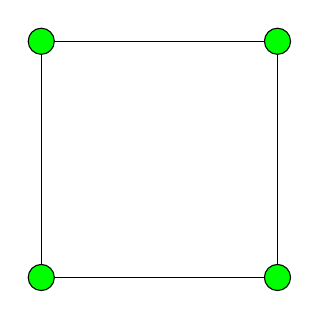
\begin{tikzpicture}[scale=1]
  \tikzstyle{every node}=[fill=green,draw,shape=circle]
  \path (0,0) node (A) {$$};
\path (0,3) node (B) {$$};
\path (3,3) node (C) {$$};
\path (3,0) node (D) {$$};
  \draw (A) -- (B)
        (B) -- (C)
        (C) -- (D)
        (D) -- (A);
\end{tikzpicture}
\caption{A 4-cycle}
  \label{cycle4}
\end{subfigure}%
\begin{subfigure}{.4\textwidth}
  \centering
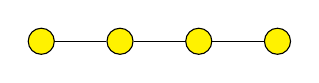
\begin{tikzpicture}[scale=1]
  \tikzstyle{every node}=[fill=yellow,draw,shape=circle]
  \path (0,0) node (A) {$$};
  \path (1,0) node (B) {$$};
  \path (2,0) node (C) {$$};
  \path (3,0) node (D) {$$};
  \draw (A) -- (B)
        (B) -- (C)
        (C) -- (D);
\end{tikzpicture}
  \caption{A 4-path}
  \label{path4}
\end{subfigure}
\caption{A 4-cycle and a 4-path}
\label{4c4p}
\end{figure}
\end{defn}

From a homogenous graph we construct a directed graph as described below. 
\begin{lemma}
If $G = (V,U)$ is decomposable and $(u,v) \in E$, then either 
\begin{align*}
\{w:w=u \text{ or } (u,w) \in E\} \subset \{w:w=v \text{ or } (v,w) \in E\}, 
\end{align*}
or
\begin{align*}
\{w:w=v \text{ or } (v,w) \in E\} \subset \{w:w=u \text{ or } (u,w) \in E\}.
\end{align*}
\end{lemma}
\begin{figure}
\centering
\begin{subfigure}{.4\textwidth}
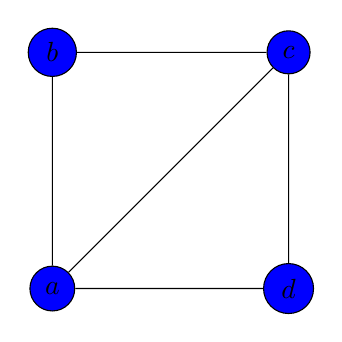
\begin{tikzpicture}[scale=1]
  \tikzstyle{every node}=[fill=blue,draw,shape=circle]
  \path (0,0) node (A) {$a$};
\path (0,3) node (B) {$b$};
\path (3,3) node (C) {$c$};
\path (3,0) node (D) {$d$};
  \draw (A) -- (B)
        (B) -- (C)
 (C) -- (A)
        (C) -- (D)
        (D) -- (A);
\end{tikzpicture}
\caption{A decomposable graph}
  \label{decomp}
\end{subfigure}%
\begin{subfigure}{.4\textwidth}
  \centering
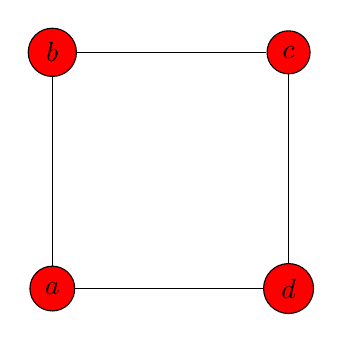
\begin{tikzpicture}[scale=1]
  \tikzstyle{every node}=[fill=red,draw,shape=circle]
  \path (0,0) node (A) {$a$};
\path (0,3) node (B) {$b$};
\path (3,3) node (C) {$c$};
\path (3,0) node (D) {$d$};
  \draw (A) -- (B)
        (B) -- (C)        
        (C) -- (D)
        (D) -- (A);
\end{tikzpicture}
  \caption{A non-decomposable graph}
  \label{nondecomp}
\end{subfigure}
\caption{A decomposable and a non-decomposable graph}
\label{decomposablegraph}
\end{figure} 
Hence either we have that $u$ or the neighbors of $u$ are contained
in $v$ or the neighbors of $v$, or vice versa. In Figure \ref{decomp},
we have that $E = \{(a,b),(b,c),(a,c),(c,d),(d,a)\}$. Also note that
if $nb(u) \coloneqq \{\text{neighbors of u}, u \in E\}$ and $N(u)
\coloneqq \{u\} \cup nb(u)$,
then 
\begin{align*}
nb(a) &= \{b,c,d\} \implies N(a)  = \{a,b,c,d\} \\
nb(b) &= \{a,c\} \implies N(b)  = \{a,b,c\}\\
nb(c) &= \{b,a,d\}\implies N(c)  = \{a,b,c,d\}\\
nb(d) &= \{a,c\} \implies N(d)  = \{a,c,d\}
\end{align*}
which implies that
\begin{align*}
N(b) \subset N(a)  \\
N(b) \subset N(c)  \\
N(a) = N(c)  \\
N(d) \subset N(c)  \\
N(d) \subset N(a) 
\end{align*} 
However, in Figure \ref{nondecomp} we have a non-decomposable graph such that $E =
\{(a,b),(b,c),(c,d),(d,a)\}$ and 
\begin{align*}
nb(a) &= \{b,d\} \implies N(a)  = \{a,b,d\}\\
nb(b) &= \{a,c\} \implies N(b)  = \{a,b,c\}\\
nb(c) &= \{b,d\} \implies N(c)  = \{b,c,d\}\\
nb(d) &= \{a,c\} \implies N(d)  = \{a,c,d\}.
\end{align*}
Here, $N(a) \not\subset N(b)$ and $N(b)
\not\subset  N(a)$. 
\begin{defn}
Let $G = (V,E)$ be a decomposable graph. Let $v \in V$.
\begin{align*}
\bar{v} \coloneqq \{w: N(v) = N(w)\}.
\end{align*}
Then
\begin{align*}
\bar{V} \coloneqq \{\bar{v}:v \in V\}
\end{align*}
and 
\begin{align*}
\bar{E} \coloneqq \{(\bar{u},\bar{v}): \bar{u}, \bar{v} \in \bar{V},
  \bar{u} \not= \bar{v}, N(u) \subsetneq N(v) \}.
\end{align*}
In such a case we write $\bar{u} \to \bar{v}$.
Then $\bar{G} = (\bar{V}, \bar{E})$ is called the \textbf{Hasse
  diagram} or \textbf{directed rooted tree} for graph $G$. 
\end{defn}
Therefore we combine all the vertices who set of neighbors are the
same into a class, $\bar{v}$. Note that this is an equivalence
relation on $V$, that is, for $a,b,c \in V$, it is reflexive $(a \sim a)$, symmetric $(a \sim b
\implies b \sim a)$ and transitive $(a \sim b \text{
  and } b \sim c \implies
a \sim c)$. In Figure \ref{decomp}, it is clear that $\bar{a} =
\{a,c\}, \bar{b} =
\{b\}$ and $\bar{d} = \{d\}$. Thus $\bar{V} =
\{\bar{a},\bar{b},\bar{d} \}$. Also we have that $N(b) \subsetneq N(a) $
and $N(d) \subsetneq N(a)$ which implies that $\bar{b} \to \bar{a}$
and $\bar{d} \to \bar{a}$. The Hasse diagram is shown in Figure
\ref{hasseg}.
\begin{figure}
\begin{center}
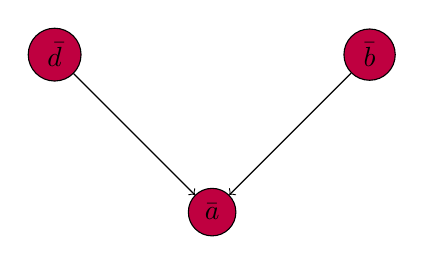
\begin{tikzpicture}[scale=2]
  \tikzstyle{every node}=[fill=purple,draw,shape=circle]
  \path (1,0) node (A) {$\bar{a}$};
\path (2,1) node (B) {$\bar{b}$};
\path (0,1) node (D) {$\bar{d}$};
\draw 
(A) edge[<-] (B)
(A) edge[<-] (D);
\end{tikzpicture}
\caption{A Hasse diagram for $G = ( \{a,b,c,d\} , \{(a,b),(b,c),(a,c),(c,d),(d,a)\}).$}
\label{hasseg}
\end{center}
\end{figure} 
\begin{defn}
A \textbf{tree}, $G$, is an undirected simple graph that satisfies any of the
following:
\begin{enumerate}
\item $G$ is connected and and has no cycles.
\item $G$ has no cycles and a simple graph is formed if any edge is
  added to $G$.
\item $G$ is connected, but is not connected if any simple edge is
  removed from $G$.
\item G is connected and $K_3$ is not a minor of $G$, i.e. we cannot
  get $K_3$ by deleting edges and vertices from $G$.
\item Any 2 vertices in $G$ can be connected by a unique simple path.
\item If $G$ has $n$ vertices, then G is connected and has $n-1$
  edges.
\item $G$ has no simples cycles and $n-1$ edges.
\end{enumerate}
\end{defn}
\begin{defn}
A \textbf{directed tree} is a tree with directed edges.
\end{defn}
\begin{defn}
A \textbf{rooted tree} is a tree where one vertex is designated as the
root and all the edges are directed either towards the root or away
from the tree.
\end{defn}
\begin{lemma}
If $G$ is homogenous, then its Hasse diagram, $\bar{G}$, is a directed
rooted tree.
\end{lemma}
Thus to find a Hasse ordering for a homogenous graph we need to carry
out the followign steps
\begin{enumerate}
\item Partition the vertices into equivalence classes.
\item Define a directed rooted tree called a Hasse diagram of G.
\end{enumerate}
\begin{defn}
Suppose $G = (V,E)$ with hasse diagram $\bar{G} =
(\bar{V},\bar{E})$. Then $u,v \in \bar{V}$ and $u \to v$ implies
that $u$ is an \textbf{ancestor} of $v$ and $v$ is a
\textbf{descentdant} of $u$.
\end{defn}
\begin{defn}
An ordering (not necessarily unique) obtained by assigning an ancestor
a higher label than any of its descendant is called a \textbf{Hasse ordering}.
\end{defn}
From Figure \ref{hasseg} we can see that some hasse orderings for Figure
\ref{decomp} would be 
\[
\begin{pmatrix} 
a & b & c & d \\
3&1&4&2 
\end{pmatrix} 
\text { or }
\begin{pmatrix} 
a & b & c & d \\
4&2&3&1 
\end{pmatrix}.
\]
\begin{thm}
Let $G = (\{1,...,p\},E)$ be a homogenous graph with a Hasse
ordering. Let 
\begin{align*}
\pg &\coloneqq \{\s:\s \in \pd \text{ and } (i,j)\not\in E \implies \s_{ij} =
      0\}\\
\mathcal{L}_G &\coloneqq \{L:L \text{ is lower triangular and } (i,j)\not\in E \implies L_{ij} =
      0\}
\end{align*}
Then
\begin{align*}
\s = LDL^T \in \pg \iff L \in \mathcal{L}_G \iff L^{-1} \in \mathcal{L}_G
\end{align*}
\end{thm}
\begin{proof}
Proof needed.
\end{proof}
The converse is also true.
\begin{thm}
Let $G = (\{1,...,p\},E)$ and 
\begin{align*}
\pg &\coloneqq \{\s:\s \in \pd \text{ and } (i,j)\not\in E \implies \s_{ij} =
      0\}\\
\mathcal{L}_G &\coloneqq \{L:L \text{ is lower triangular and } (i,j)\not\in E \implies L_{ij} =
      0\}
\end{align*}
Suppose that 
\begin{align*}
&\s = LDL^T \in \pg, \\ 
&L \in \mathcal{L}_G \text{ and }\\
&L^{-1} \in \mathcal{L}_G.
\end{align*}
Then $G$ is homogenous with a Hasse ordering. 
\end{thm}
\begin{proof}
Proof needed.
\end{proof}

\subsection{Closed form of $\hat{\s}_{mle}$}
To find $\hat{\s}_{mle}$ we have to solve the following problem:
\begin{align*}
\hat{\s}_{mle} &= \arg \min_{\s \in \pg} l^*(\s) \\
 &= \arg \min_{\s \in \pg} tr(\s^{-1}S) + \log \abs{\s}
\end{align*}
Now if $G$ is homogenous, then $\s = LDL^T \implies \s^{-1} = L^{-T}D^{-1}L^{-1} $ where $L \in
\mathcal{L}_G$ and 
\begin{align*}
D \in \mathcal{D} = \{D: D \text{ is a diangonal matrix such that }
  \forall i,d_{ii}>0\}
\end{align*}
Thus 
\begin{align*}
l^*(L,D) = tr(L^{-T}D^{-1}L^{-1}S) + \log \abs{D}
\end{align*}
Now let $T \coloneqq L^{-1}$.
Then
\begin{align*}
l^*(T,D) &= tr(T^{T}D^{-1}TS) + \log \abs{D} \\ 
&= tr(D^{-1}TST^{T}) + \log \prod_{i=1}^p D_{ii} \\ 
&= \sum_{i=1}^p(D^{-1}TST^{T})_{ii} + \sum_{i=1}^p \log D_{ii} \\ 
&= \sum_{i=1}^p (\frac{T_{i.}(ST^{T})_{.i} }{D_{ii}}+ \log
  D_{ii})\\
&= \sum_{i=1}^p (\frac{T_{i.}S(T^{T})_{.i} }{D_{ii}}+ \log
  D_{ii}) \\
&= \sum_{i=1}^p (\frac{T_{i.}S T_{i.}^T}{D_{ii}}+ \log
  D_{ii}) 
\end{align*}
Thus we can minimize with respect to $T_{i.}$ and $D_{ii}$ separately
for each $i$. Note that if $x^i = (t_{ij})_{j<i,(i,j) \in E}$, then 
\begin{align*}
T_{i.}ST_{i.}^T 
&= \sum_{j=1}^p \sum_{k=1}^p S_{jk}t_{ij}t_{ik}\\
&= \sum_{j=1,(i,j) \in E}^i \sum_{k=1,(i,k) \in E}^i
  S_{jk}t_{ij}t_{ik} \quad \text { as } (i,j) \not\in E \implies t_{ij}=0\\
&= (x^i,1)
\begin{pmatrix} 
S^{<i} & S^{<}_{.i} \\
(S^{<}_{.i})^T& S_{ii} 
\end{pmatrix}
\begin{pmatrix} 
x^i\\1
\end{pmatrix}\\
&= (x^i)^T S^{<i} x^i + (x^i)^T S^{<}_{.i} + (S^{<}_{.i})^T x^i + S_{ii}
\end{align*}
where 
\begin{align*}
S^{<}_{.i} &= (S_{k,i})_{k<i,(i,k) \in E} \\
N^<(i) &= \{j:j<i,(i,j) \in E\}\\
S^{<i} &= (S_{k,l})_{k,l<i, k,l \in N^<(i)} 
\end{align*}
Note that to minimize $T_{i.}ST_{i.}^T$ we can simply take the
derivative with respect to $x^i$
\begin{align*}
&\frac{\partial}{\partial x^i} T_{i.}ST_{i.}^T\\ 
&= \frac{\partial}{\partial x^i} (x^i)^T S^{<i} x^i + (x^i)^T
  S^{<}_{.i} + (S^{<}_{.i})^T x^i + S_{ii} \\
&= 2  S^{<i} x^i + 2S^{<}_{.i} \overset{set}{=} 0 \\
\implies \hat{x}^i &= (S^{<i})^{-1}S^{<}_{.i} \\
\implies \hat{T}_{i.}S \hat{T}_{i.}^T &= (\hat{x}^i)^T S^{<i} \hat{x}^i +
                           (\hat{x}^i)^T S^{<}_{.i} + (S^{<}_{.i})^T
                           \hat{x}^i + S_{ii} \\
&= + (S^{<}_{.i})^T (S^{<i})^{-1}S^{<}_{.i} -  (S^{<}_{.i})^T
  (S^{<i})^{-1} S^{<}_{.i} -  (S^{<}_{.i})^T
  (S^{<i})^{-1} S^{<}_{.i} + S_{ii} \\
&= S_{ii} -  (S^{<}_{.i})^T
  (S^{<i})^{-1} S^{<}_{.i}
\end{align*}
If we define
\begin{align*}
S_i = \begin{pmatrix} 
S^{<i} & S^{<}_{.i} \\
(S^{<}_{.i})^T& S_{ii} 
\end{pmatrix},
\end{align*}
then 
\begin{align*}
l^*(T,D) &= tr(T^{T}D^{-1}TS) + \log \abs{D} \\ 
&= \sum_{i=1}^p (\frac{T_{i.}S T_{i.}^T}{D_{ii}}+ \log
  D_{ii}) \\
&= \sum_{i=1}^p [\frac{1}{D_{ii}}((x^i,1)
S_i
\begin{pmatrix} 
x^i\\1
\end{pmatrix})+ \log
  D_{ii}].
\end{align*}
Also note that $\frac{\partial}{\partial
  D_{ii}}(\frac{c}{D_{ii}}+\log{D_{ii}}) = -\frac{c}{D_{ii}^2} +
\frac{1}{D_{ii}} \overset{set}{=} 0 \implies D_{ii} = c$. Thus the
value of $D_{ii}$ that minimizes $l^*(T,D)$ is $S_{ii} -  (S^{<}_{.i})^T
  (S^{<i})^{-1} S^{<}_{.i}$.
\begin{lemma}
\begin{align*}
\hat{\s} = \Big[\sum_{i=1}^p[S_i^{-1}]^0-\sum_{i=1}^p[(S^{<i} )^{-1}]^0 \Big]^{-1}
\end{align*}
\end{lemma}
\begin{proof}
We do the proof for $p = 3$. Let $S = (s_{ij})$. Then we have that 
\begin{align*}
S_1 &= s_{11} \\
S_2 &= 
\begin{pmatrix}
s_{11} & s_{12}\\
s_{21} & s_{22}
\end{pmatrix} \\
S^{<2} &= s_{11} = S_1\\
S_3 &= S\\
S^{<3} &= \begin{pmatrix}
s_{11} & s_{12}\\
s_{21} & s_{22}
\end{pmatrix}  = S_2
\end{align*}
Thus 
\begin{align*}
\hat{\s} &= \Big[\sum_{i=1}^p[S_i^{-1}]^0-\sum_{i=1}^p[(S^{<i} )^{-1}]^0
  \Big]^{-1} \\
&= \Big[[S_1^{-1}]^0-[(S^{<2} )^{-1}]^0+[S_2^{-1}]^0-[(S^{<3} )^{-1}]^0+[S_3^{-1}]^0
  \Big]^{-1} \\
&= \Big[[S_1^{-1}]^0-[S_1^{-1}]^0+[S_2^{-1}]^0-[S_2^{-1}]^0+[S_3^{-1}]
  \Big]^{-1} \\
&= S_3 = S.
\end{align*}
\end{proof}

\subsection{Direct sample from $\mathcal{GIW}(U,\delta)$ for
  homogenous graphs}
Recall that the pdf of the $\mathcal{GIW}(U,\delta)$ is proportional
to
\begin{align*}
\pi_{U,\delta}(\s) \propto
  e^{-\frac{1}{2}tr(\s^{-1}U)-\frac{\delta}{2}\log \abs{\s}}, \s \in \pg
\end{align*}
Assume $G$ is homogenous. Then there is a Hasse ordering for the
vertices of $G$ and suppose 
\begin{align*}
\s &= LDL^{T} \\
T &= L^{-1}, T \in \mathcal{L}_{\mathcal{G}} \\
\implies \s & \mapsto (L,D) \text{ is a bijection} \\ & (L,D) \mapsto (T,D) \text{ is a bijection}
\end{align*}
where the determinant of $\s \mapsto (L,D)$ is $\prod_{j=1}^p
D_{jj}^{n_j}, n_j = \abs{\{i:i>j,(i,j) \in E\}}$ and the determinant
of $(L,D) \mapsto (T,D)$ is 1.
Therefore, 
\begin{align*}
\pi_{U,\delta}(T,D) &\propto
  e^{-\frac{1}{2}tr(T^T D^{-1} T U)-\frac{\delta}{2}\log \abs{D}} \prod_{j=1}^p
D_{jj}^{n_j}\\
&= e^{-\sum_{i=1}^p \frac{(TUT^T)_{ii}}{2D_{ii}}-sum_{i=1}^p
  (\frac{\delta-2n_i}{2})\log D_{ii}} 
\end{align*}

The sampling strategy will be to first draw from $T|D$ and then sample
from the marginal distribution of $D$. Let
\begin{align*}
U^{<i} &= ((U_{kl}))_{k<i,l<i,(k,i)\in E, (k,l) \in E} \\
x^i &= (T_{ij})_{j<i,(i,j) \in E,2 \leq i \leq p} \\
U_i &= \begin{pmatrix} U^{<i} & U_{.i}^{<i} \\ (U_{.i}^{<i})^T &
  U_{ii} \end{pmatrix}
\end{align*}
Then, 
\begin{align*}
\pi_{U,\delta}(T,D) 
&= e^{-\sum_{i=1}^p \frac{(TUT^T)_{ii}}{2D_{ii}}-sum_{i=1}^p
  (\frac{\delta-2n_i}{2})\log D_{ii}} \\
&= e^{-\frac{1}{2D_{ii}} \sum_{i=1}^p \begin{pmatrix} (x^i)^T &
    1\end{pmatrix} U_i \begin{pmatrix} (x^i)^T \\ 1\end{pmatrix} +
  \sum_{i=1}^p (\frac{\delta-2n_i}{2}) \log D_{ii}}
\end{align*}
\subsection{Graphical Lasso}
Let 
\[
Q_{GL}(\om) = tr(\om S) - \log \abs{\om} + \lambda \sum_{1\leq i<j
  \leq p} \abs{\om_{ij}}, \quad \om \in \pg
\]
denote the objective function for graphical lasso. We want to find
$\hat{\om}$ such that $Q_{GL}(\hat{\om}) = \arg\min_{\om \in \pg}
Q_{GL}({\om})$. Fix $i \in \{ 1,...,p \}$. Let
\begin{align*}
\om_{-i,i} &= (\om_{ji})_{j\not=i}\\
\om_{-i,-i} &= (\om_{kl})_{k,l\not=i}\\
\gamma_i &= \om_{i,i} - \om_{i,-i}\om_{-i,-i}^{-1}\om_{-i,i}
\end{align*}
Then 
\[
\om \mapsto (\om_{-i,i},\om_{-i,-i},\gamma_i )
\]
is a bijection.
An $\ell_1$ penalty, as we have here, imposes both sparsity and shrinkage as
opposed to a ridge penalty which imposes only shrinkage. Also, as $\abs{\om} = \abs{\om_{-i,-i}}\abs{\gamma_i}$ by
Equation \ref{eq:schurdet},
\begin{align*}
Q_{GL}(\om) &= tr(\om S) - \log \abs{\om} + \lambda \sum_{1\leq i<j
  \leq p} \abs{\om_{ij}} \\
&= tr\Big(
\begin{pmatrix} \om_{i,i} & \om_{i,-i} \\
\om_{-i,i} & \om_{-i,-i} \\
\end{pmatrix}
\begin{pmatrix} S_{i,i} & S_{i,-i} \\
S_{-i,i} & S_{-i,-i} \\
\end{pmatrix}
  \Big) - \log \abs{\om_{-i,-i}}\abs{\gamma_i}\\ &\qquad + \lambda \sum_{1\leq i<j
  \leq p} \abs{\om_{ij}} \\
&= tr\Big(
\begin{pmatrix} \om_{i,i} & \om_{i,-i} \\
\om_{-i,i} & \om_{-i,-i} \\
\end{pmatrix}
\begin{pmatrix} S_{i,i} & S_{i,-i} \\
S_{-i,i} & S_{-i,-i} \\
\end{pmatrix}
  \Big) - \log \abs{\om_{-i,-i}} - \log\abs{\gamma_i} \\ 
&\qquad + \lambda
  {\norm{\om_{-i,i}}}_1 + \text{ other terms depending on }
  \om_{-i,-i} \\
&= tr(
\om_{i,i} S_{i,i} + \om_{i,-i}S_{-i,i}  +
\om_{-i,i} S_{i,-i} + \om_{-i,-i} S_{-i,-i} ) - \log\abs{\gamma_i} \\ 
&\qquad + \lambda
  {\norm{\om_{-i,i}}}_1 + \text{ other terms depending on }
  \om_{-i,-i} \\
&= tr(
\gamma_i S_{i,i} + \om_{i,-i}\om_{-i,-i}^{-1}\om_{-i,i}S_{i,i} + \om_{i,-i}S_{-i,i}  +
\om_{-i,i} S_{i,-i} ) \\ 
&\qquad + \lambda
  {\norm{\om_{-i,i}}}_1 + \text{ other terms depending on }
  \om_{-i,-i}, \gamma_i \\
&= \om_{i,-i}\om_{-i,-i}^{-1}\om_{-i,i}S_{i,i} +
  2\om_{i,-i}S_{-i,i} 
\\ 
&\qquad + \lambda
  {\norm{\om_{-i,i}}}_1 + \text{ other terms depending on }
  \om_{-i,-i}, \gamma_i 
\end{align*}
as $tr(\om_{i,-i}S_{-i,i}) =
  \om_{i,-i}S_{-i,i} = \om_{-i,i}S_{i,-i} \in \mathbb{R}$ and
  $tr(\om_{i,-i}\om_{-i,-i}^{-1}\om_{-i,i}S_{i,i} ) =
  \om_{i,-i}\om_{-i,-i}^{-1}\om_{-i,i}S_{i,i} \in \mathbb{R}$.
Thus, as $S_{i,i}$ is a constant
\begin{align*}
\implies Q_{GL}(\om|\om_{-i,i},\gamma_i) &= 
\om_{-i,i }^T (S_{i,i}\om_{-i,-i}^{-1})\om_{-i,i} +
2\om_{-i,i} S_{i,-i} + \lambda
  \norm{\om_{-i,i}}_1 
\end{align*}
which implies that keeping $\gamma_i$ and $\om_{-i,-i}$ fixed and then
minimizing $Q_{GL}$ with respect to $\om_{i,-i}$ is equivalent to a
regression lasso problem. 
Similarly we can show that
\begin{align*}
\implies Q_{GL}(\gamma_i|\om_{-i,i},\om_{-i,-i}) &= 
\gamma_i S_{i,i} - \log{\gamma_i}
\end{align*}
which is minimized at $\hat{\gamma}_i = \frac{1}{S_{ii}}$.
We can use coordinate-wise minimization to update $\gamma_i$ and
$\om_{-i,i}$ for $i = 1,...,p$. Convergence is guaranteed by convexity
of the objective function. In general, the algorithm is
$O(p^4)$ as each iteration involves inverting a $(p-1) \times (p-1)$ matrix, which
is $O(p-1)^3 \approx O(p^3)$ and there are $p$ iterations in total.
\subsection{SPACE algorithm}
This is due to Peng et.al. (2009) in JASA. The main idea here is to
change the objective function by replacing the likelihood with the
psuedolikelihood, which is the product of full conditionals. Note that
if $Y = (Y_1,...Y_p) \distas{} \mathcal{N}_p(0,\s = \om^{-1})$, then
\begin{align*}
Y_1|Y_{-1} \distas{} \mathcal{N}(\s_{1,-1}\s_{-1,-1}^{-1}(Y_{-1}),\s_{1,1}-\s_{1,-1}\s_{-1,-1}^{-1}\s_{-1,1})
\end{align*}
where 
\begin{align*}
\s = \begin{pmatrix} \s_{1,1} & \s_{1,-1} \\
\s_{-1,1}& \s_{-1,-1}\end{pmatrix}
\text { and } 
\om = \begin{pmatrix} \om_{1,1} & \om_{1,-1} \\
\om_{-1,1}& \om_{-1,-1}\end{pmatrix}
\end{align*}
As $\s_{-1,-1}$ is invertible we have by using Schur Complements that 
\[
\Scale[0.75]{
\s^{-1} = \begin{pmatrix}
  (\s_{1,1}-\s_{1,-1}\s_{-1,-1}^{-1}\s_{-1,1})^{-1}&
  -(\s_{1,1}-\s_{1,-1}\s_{-1,-1}^{-1}\s_{-1,1})^{-1} \s_{1,-1} \s_{-1,-1}^{-1} \\
-\s_{-1,-1}^{-1}\s_{-1,1}
(\s_{1,1}-\s_{1,-1}\s_{-1,-1}^{-1}\s_{-1,1})^{-1} &
\s_{-1,-1}+\s_{-1,-1}^{-1}\s_{-1,1}(\s_{1,1}-\s_{1,-1}\s_{-1,-1}^{-1}\s_{-1,1})^{-1}\s_{-1,1}\s_{-1,-1}^{-1} 
\end{pmatrix}}
\]
Hence,
\begin{align*}
 \om_{11}
&=(\s_{1,1}-\s_{1,-1}\s_{-1,-1}^{-1}\s_{-1,1})^{-1}\\ 
\om_{1,-1} 
&=
-(\s_{1,1}-\s_{1,-1}\s_{-1,-1}^{-1}\s_{-1,1})^{-1} \s_{1,-1}
\s_{-1,-1}^{-1} \\
\implies -(\om_{1,1})^{-1} \om_{1,-1} &=
(\s_{1,1}-\s_{1,-1}\s_{-1,-1}^{-1}\s_{-1,1}) \\
& \quad \times (-(\s_{1,1}-\s_{1,-1}\s_{-1,-1}^{-1}\s_{-1,1})^{-1}
  \s_{1,-1}\s_{-1,-1}^{-1}) \\
&= - \s_{1,-1}\s_{-1,-1}^{-1}
\end{align*}
 This gives us the following lemma:
\begin{lemma}
\label{lemma:regrcoeffs} $\s_{i,-i}\s_{-i,-i}^{-1} =
-(\om_{ii})^{-1} \om_{i,-i}$.
\end{lemma}
This tells us that 
\begin{align*}\s_{1,-1}\s_{-1,-1}^{-1}(Y_{-1}) &=
-(\om_{11})^{-1} \om_{1,-1}(Y_{-1})\\ &=
-\frac{1}{\om_{11}}(\om_{12},...,\om_{1p})
\begin{pmatrix}
Y_2\\
\vdots\\
Y_p
\end{pmatrix} \\
&= -\sum_{j \not= 1} \frac{\om_{j1}}{\om_{11}} Y_j
\end{align*}
In general,
\begin{align*}
Y_i|Y_{-i} \distas{} \mathcal{N}(-\sum_{j \not= i} \frac{\om_{ji}}{\om_{ii}} Y_j,\frac{1}{\om_{ii}}).
\end{align*}
Thus the psuedolikelihood is 
\begin{align*}
p(\om) &= \prod_{k=1}^n \prod_{i=1}^p f_{Y_i|Y_{-i}}(Y_i^k) \\ &= \prod_{k=1}^n \prod_{i=1}^p
  \frac{\sqrt{\om_{ii}}}{\sqrt{2 \pi }}e^{-\frac{\om_{ii}}{2}(Y_i^k - (-\sum_{j \not= i} \frac{\om_{ji}}{\om_{ii}} Y_j^k))^2}
\end{align*}
and the negative log of the psuedolikelihood is 
\begin{align*}
- \log p(\om) &= \sum_{k=1}^n\sum_{i=1}^p \{ \frac{\om_{ii}}{2}(Y_i^k - (-\sum_{j
  \not= i} \frac{\om_{ji}}{\om_{ii}} Y_j^k))^2 - \frac{1}{2}
                \log{\om_{ii}}\} \\
&= \sum_{i=1}^p \{ \frac{\om_{ii}}{2} \sum_{k=1}^n (Y_i^k - (-\sum_{j
  \not= i} \frac{\om_{ji}}{\om_{ii}} Y_j^k))^2 - \frac{n}{2}
                \log{\om_{ii}}\} \\
&= \sum_{i=1}^p \{ \frac{\om_{ii}}{2} \sum_{k=1}^n (\sum_{j
  =1}^p \frac{\om_{ji}}{\om_{ii}} Y_j^k))^2 - \frac{n}{2}
                \log{\om_{ii}}\} \\
&= \sum_{i=1}^p \{ \frac{\om_{ii}}{2} \frac{1}{\om_{ii}^2}\sum_{k=1}^n (\sum_{j
  =1}^p {\om_{ji}}Y_j^k))^2 - \frac{n}{2}
                \log{\om_{ii}}\} \\
&= \sum_{i=1}^p \{ \frac{\om_{ii}}{2} \frac{1}{\om_{ii}^2}\sum_{k=1}^n
  ({\om_{1i}}Y_1^k + ... + {\om_{pi}}Y_p^k)^2 - \frac{n}{2}
                \log{\om_{ii}}\} \\
&= \sum_{i=1}^p \{ \frac{\om_{ii}}{2} \frac{1}{\om_{ii}^2}\sum_{k=1}^n
  ((Y^k)^T \om_{.i})^2 - \frac{n}{2}
                \log{\om_{ii}}\} \\
&= \sum_{i=1}^p \{ \frac{\om_{ii}}{2} \frac{1}{\om_{ii}^2}
 \sum_{k=1}^n ((Y^k)^T \om_{.i})^T((Y^k)^T \om_{.i}) - \frac{n}{2}
                \log{\om_{ii}}\} \\
&= \sum_{i=1}^p \{ \frac{\om_{ii}}{2} \frac{1}{\om_{ii}^2}
  \om_{.i}^T nS \om_{.i} - \frac{n}{2}
                \log{\om_{ii}}\} \\
\end{align*}
Thus for one observation the negative log psuedolikelihood is
\begin{align*}
&= \sum_{i=1}^p \{ \frac{\om_{ii}}{2} \frac{1}{\om_{ii}^2}
  \om_{.i}^T S \om_{.i} - \frac{1}{2}
                \log{\om_{ii}}\} \\
\end{align*}
Note that we can also write 
\begin{align*} 
- \log p(\om) &= \sum_{k=1}^n\sum_{i=1}^p \{ \frac{\om_{ii}}{2}(Y_i^k - (-\sum_{j
  \not= i} \frac{\om_{ji}}{\om_{ii}} Y_j^k))^2 - \frac{1}{2}
                \log{\om_{ii}}\} \\
&= \sum_{i=1}^p \{ \frac{\om_{ii}}{2} \norm{(Y_i^k - (-\sum_{j
  \not= i} \frac{\om_{ji}}{\om_{ii}} Y_j^k))}_2^2 - \frac{n}{2}
                \log{\om_{ii}}\} 
\end{align*} 
If the main objective is to estimate the sparsity pattern, then the
restriction $\om \in \pg$ or $\om \in \pd$ is not needed.
Define 
\begin{align*}
\beta_{ij} &= -\frac{\om_{ij}}{\om_{ii}}\\
\beta &= (\beta_{ij})_{1\leq i < j\leq p}
\end{align*}
and the partial correlation coefficient
\begin{align*}
\rho_{ij} &= \frac{\om_{ij}}{\sqrt{\om_{ii}\om_{jj}}}\\
\rho &= (\rho_{ij})_{1\leq i < j\leq p}
\end{align*}
Then
\begin{align*}
\om \mapsto (\beta,(\om_{ii})_{i=1}^p) \mapsto (\rho,(\om_{ii})_{i=1}^p)
\end{align*}
are all bijections, which means that sparsity in $\om$ is equivalent
to sparsity in $\rho$ and $\beta$.
Thus if $Y^1,...,Y^n \distas{iid} \mathcal{N}_p(0, \s = \om^{-1})$,
let $Y_i = (Y_i^1,...,Y_i^n)$ is the $i$-th component of all the
observations put into a $n \times 1$ vector. Then the objective
function of the SPACE algorithm is:
\begin{align*}
Q_{SPACE}(\rho,(\om_{ii})_{i=1}^p) = 
\sum_{i=1}^p \frac{\om_{ii}}{2} \norm{Y_i - (-\sum_{j
  \not= i} \beta_{ij} Y_j)}_2^2 &- \frac{n}{2} \sum_{i=1}^p \log
                                    (\om_{ii}) \\
& \quad + \lambda \sum_{1 \leq
                                    i < j \leq p} \abs{\rho_{ij}}
\end{align*}
We can fo the minimization of the objective function in two
steps. First fix $\om$ and estimate $\beta$ by adaptive lasso
regressions. Then fix $\beta$, which has a closed form solution. One
thing to note is that postive definiteness is lost in this approach,
but that is of little concern as the main interest here is the
sparsity pattern. The objective function
$Q_{SPACE}(\rho,(\om_{ii})_{i=1}^p)$ is not jointly convex, but is
bi-convex, which means that it is convex in each part keeping the
other part constant. As a result, we can construct some examples where the SPACE
algorithm does not converge.
\begin{algorithm}  
\caption{SPACE pseudocode}
\begin{algorithmic}
\State Input: Standardize data to have mean zero and standard deviation one
\State Input: Fix maximum number of iterations: $r_{max}$
\State Input: Fix initial estimate: $\hat{\om}_{ii}^{(0)} =
  \frac{1}{S_{ii}}$ as suggested
\State Input: Choose weights: $w_i (w_i = \om_{ii} \text{ or } w_i = 1)$
\State Set $r \gets 1$
\Repeat
\State \Comment{update partial correlations} 
\State Update $\hat{\rho}^{(r)}$ by minimizing (with current estimates $\{
  \hat{\om}_{ii}^{(r-1)} \}_{i=1}^p$)
\For{$i = 1,...,p$}
\State \begin{align*}
\frac{1}{2}(\sum_{i=1}^p w_i \norm{Y_i - (-\sum_{j
  \not= i} \rho_{ij} \sqrt{\frac{\om_{jj}^{(r-1)}}{\om_{ii}^{(r-1)}}} Y_j)}_2^2) + \lambda \sum_{1 \leq
                                    i < j \leq p}
                                  \abs{\rho_{ij}}
\end{align*} 
\State \Comment{update conditional variance} 
\State Update $\{ \om_{ii}^{(r)} \}_{i=1}^p$ by computing (with fixed
  estimates $\{ \hat{\rho}_{ij}^{(r-1)}\}$
\State and $\{
  \hat{\om}_{ii}^{(r-1)} \}_{i=1}^p$)
\State {\begin{align*}
\frac{1}{\hat{\om}_{ii}^{r}} = \frac{1}{n} \norm{Y_i - (-\sum_{j
  \not= i} \hat{\rho}_{ij}^{(r-1)}
  \sqrt{\frac{\om_{jj}^{(r-1)}}{\om_{ii}^{(r-1)}}} Y_j)}_2^2\end{align*}}
\EndFor
\State $r \gets r+1$ 
\State Update weights: $w_i$
\Until $r==r_{max}$
\State \Return $(\hat{\rho}^{(r_{max)}},\{\hat{\om}_{ii}^{(r_{max})} \}_{i=1}^{p})$
\end{algorithmic}
\end{algorithm}

\subsection{CONCORD algorithm} This is due to Khare, Oh and
Rajaratnam (2014) in JRSSB. First note that the objective function of
the SPACE algorithm can be rewritten as:
\begin{align*}
Q_{SPACE}(\om) = \frac{n}{2} \sum_{i=1}^p
  \frac{w_i}{\om_{ii}^2}(\om_{.i}^TS \om_{.i}) - \frac{n}{2}
  \sum_{i=1}^p \log (\om_{ii}) + \lambda \sum_{1 \leq i < j \leq p} \abs{\frac{\om_{ij}}{\sqrt{\om_{ii}\om_{jj}}}}
\end{align*}
where $w_i$ is a weight variable. Peng et. al. suggest using $w_i = 1$
or $w_i = \om_{ii}$, but neither choice guarantees convergence. 
The main idea of CONCORD is to make some adjustment to
$Q_{SPACE}(\om)$ to make it jointly convex. The changes in
$Q_{SPACE}(\om)$ to make it resemble -2loglikelihood plus a  penalty term
are listed below:
\begin{enumerate}
\item $w_i = \om_{ii}^2$
\item change $\abs{\frac{\om_{ij}}{\sqrt{\om_{ii}\om_{jj}}}}$ with $\om_{ij}$
\item multiply $\frac{1}{2}
  \sum_{i=1}^p \log (\om_{ii})$ by 2
\end{enumerate}
Thus the objective function for the CONCORD algorithm is
\begin{align*}
Q_{CONCORD}(\om) &= \frac{n}{2}\sum_{i=1}^p
  (\om_{.i}^TS \om_{.i}) - 
   n \sum_{i=1}^p \log (\om_{ii}) + \lambda \sum_{1 \leq i < j \leq p}
  \abs{\om_{ij}} 
\end{align*}
If $i \not= j$, then 
\begin{align*}
Q_{CONCORD}(\om_{ij}|\om_{-(ij)}) &= \frac{n}{2} (S_{ii}+S_{jj})\om_{ij}^2 +
                                    n (\sum_{k\not=i} \om_{ik}S_{jk} +
                                    \sum_{k\not=j} \om_{jk}S_{ik})
                                    \om_{ij} + \lambda \abs{\om_{ij}}
  \\
&\quad + \text{ terms not depending on } \om_{ij},
\end{align*}
which look like a $lasso$ problem.
If $i = j$, then 
\begin{align*}
Q_{CONCORD}(\om_{ii}|\om_{-(ii)}) &= \frac{n}{2}
                                    S_{ii}\om_{ii}^2+n(\sum_{k\not=i}
                                    S_{ik}\om_{ki} )\om_{ii} -  n\log(\om_{ii}) \\
&\quad +  \text{ terms not depending on } \om_{ii} \\
\implies \frac{d}{d\om_{ii}} Q_{CONCORD}(\om_{ii}|\om_{-(ii)}) &=
                                                                 n\om_{ii}S_{ii}+
                                                                 n(\sum_{k\not=i}
                                                                 S_{ik}\om_{ki})
                                                                 -\frac{n}{\om_{ii}} 
                                                                 \overset{\text{set}}{=}0.
\end{align*}
Thus,
\begin{align*}\om_{ii}^2
                                                                 S_{ii}
                                                                 +
                                                                 (\sum_{k\not=i}
                                                                 S_{ik}\om_{ki})
  \om_{ii}                                                               -
                                                                 1 =
                                                                 0, 
\end{align*}
which implies that
\begin{align*}
\om_{ii} = \frac{- \sum_{k\not=i}
                                                                 S_{ik}\om_{ki}
  \pm \sqrt{(\sum_{k\not=i}
                                                                 S_{ik}\om_{ki})^2
  + 4 S_{ii}}}{2 S_{ii}}. 
\end{align*}
As $\om_{ii}>0$, 
\[
\om_{ii} = \frac{- \sum_{k\not=i}
                                                                 S_{ik}\om_{ki}
  + \sqrt{(\sum_{k\not=i}
                                                                 S_{ik}\om_{ki})^2
  + 4 S_{ii}}}{2 S_{ii}}.
\]
We now iterate the above 2-stage optimization for $i=1,...,p$ until
convergence. The computational cost for each iteration is
$min\{O(np^2),O(p^3)\}$ and the algorithm has consistent results in
high-dimensional settings. Additionally, if $n>p$, then $Q_{CONCORD}$
is strictly convex. If $n<p$, then $Q_{CONCORD}$ is no longer strictly
convex. However, convergence can still be established rigorously, even
though the starting point or initial value may be a factor.  
Note that we can also write the objective function of CONCORD as:
\begin{align*}
Q_{CONCORD}(\om)&= \frac{1}{2} \sum_{i=1}^p \norm{\om_{ii}Y_i + \sum_{j \not= i} \om_{ij}Y_j}_2^2
  - n \sum_{i=1}^p \log (\om_{ii}) + \lambda \sum_{1 \leq i < j \leq p}
  \abs{\om_{ij}} 
\end{align*}
We now restate the above results formally as a lemma, which is exactly the same
as Lemma 4 in the paper. Let $\mathcal{A}_p$ denote the set of $p \times p$  real
symmetric matrices. Let the parameter space $\mathcal{M}$ be defined as
\[
\mathcal{M} \coloneqq \{\om \in \mathcal{A}: \om_{ii}>0 \forall
1\leq\leq p \}
\]
For $1 \leq i \leq j \leq p$, define $T_{ij}:\mathcal{M} \mapsto
\mathcal{M}$ by 
\[
T_{ij}(\om) = \arg\min_{\tilde{\om}:\tilde{\om}_{kl}=\om_{kl}\forall
  (k,l)\not= (i,j)} Q_{CONCORD}(\tilde{\om}).
\]
Thus for each $(i,j)$, $T_{ij}(\om)$ gives the matrix where all the
elements of $\om$ are left as is except the $(i,j)$-th element. The
$(i,j)$-th element is replaced by the value that minimizes
$Q_{CONCORD}(\om)$ with respect to $\om_{ij}$ holding all other
variables $\om_{kl}, (k,l) \not= (i,j)$ constant. 
\begin{lemma}
\label{lemma:concordsoln}
The function $T_{ij}(\om)$ defined above can be computed in closed
form. In particular for $1\leq i \leq p$,
\[
(T_{ii}(\om))_{ii} = \frac{- \sum_{k\not=i}
                                                                 S_{ik}\om_{ki}
  + \sqrt{(\sum_{k\not=i}
                                                                 S_{ik}\om_{ki})^2
  + 4 S_{ii}}}{2 S_{ii}}.
\]
For $1 \leq i < j \leq p$
\[
(T_{ij}(\om))_{ij} = \frac{S_{\frac{\lambda}{n}}(-(\sum_{j\not=j'}\om_{ij'}S_{jj'}+\sum_{i'\not=i}\om_{i'j}S_{ii'}))}{S_{ii}+S_{jj}}
\]
where $S_{\lambda}(s) \coloneqq sign(x)(\abs{x}-\lambda)_{+}$ is the
soft-thresholding operator. 
\end{lemma}
\begin{algorithm}
\caption{CONCORD pseudocode}    
\begin{algorithmic}            
\State Input: Standardize data to have mean zero and standard deviation one
\State Input: Fix maximum number of iterations: $r_{max}$
\State Input: Fix initial estimate: $\hat{\om}_{ii}^{(0)} =$
\State Input: Fix convergence threshold: $\epsilon$ 
\State Set $r \gets 1$
\State Set converged = FALSE
\Repeat 
\State $\hat{\om}^{old} = \hat{\om}^{current}$ 
\State \Comment{updates to partial covariances $\om_{ij}$}
\For{$i = 1,...p-1$}
\For{$j = 1,...p-1$}
{\begin{align*}
\qquad \quad \quad \hat{\om}_{ij}^{current} = (T_{ij}(\om^{current}))_{ij}
\end{align*} }
\EndFor 
\EndFor 
\Comment{updates to partial variances $\om_{ii}$}
\For{$i = 1,...p-1$}
{\begin{align*}
\qquad \quad \quad \hat{\om}_{ii}^{current} =
                (T_{ii}(\om^{current}))_{ii} 
\end{align*} }
\EndFor 
\Comment{Convergence checking}
\If{$\norm{\hat{\om}^{old} -\hat{\om}^{current}}_{max} <
  \epsilon$}
\State converged = TRUE 
\Else 
\State $r \gets r+1$
\EndIf 
\Until converged=TRUE or $r>r_{max}$
\State \Return $(\hat{\om^{(r)}})$
\end{algorithmic}
\end{algorithm}
\end{document}